\chapter{Searching for High Mass Resonances in Dielectron Final State}\label{chap:Zprime}
In order to address the shortcoming of the standard model (SM), there are several theories beyond the SM predicting the existence of heavy resonances at the TeV scale that can couple to quarks or gluons and can decay to dilepton pairs. We present in this chapter a search for high mass resonances in the dielectron final state. This analysis uses proton-proton collision data at the centre-of-mass energy of 13 TeV collected by the CMS experiment in 2016 and 2017, corresponding to an integrated luminosity of 35.9 \fbinv and 41.4 \fbinv respectively. The strategy of the analysis is looking for a ``bump'' in the dielectron invariant mass distribution, in particular in the high mass tail. The data and MC samples are described in Section \ref{sec:Zprime_data_mc}. Introduction to the triggers used is presented in Section \ref{sec:Zprime_trigger}. The object and event selection are expressed in Section \ref{sec:Zprime_HEEP}. The mass scale and resolution studies are introduced in Section \ref{sec:mass_res}. The measurement of High Energy Electron Pair selection efficiency is presented in Section \ref{sec:Zprime_SF}. The SM backgrounds estimation is expressed in Section \ref{ZP_SM_background}. In Section the final dielectron invariant mass spectra are given. Finally, the statistical interpretation is presented in Section \ref{sec:Zprime_Limit}.

%%\section{Introduction}\label{sec:Zprime_intro}

\section{Data and MC samples}\label{sec:Zprime_data_mc}
The name and integrated luminosity of the all datasets used in this analysis are summarized in Table \ref{tab:Zprime-data-samples}. The DoubleEG dataset requires at least two trigger level electrons or photons for each event and it is used for main analysis. The SingleElectron dataset requires at least one trigger level electron for each event and it is used for trigger efficiency and electron selection efficiency measurement. The SingleMuon dataset requires at least one trigger level muon for each event and it is used for $\mathrm{t\bar{t}}$ background cross check using $\mathrm{'e\mu'}$ method. The SinglePhoton dataset requires at least one trigger level photon for each event and it is used for fake electron study. Form eras 2016B through 2016G and 2017B through 2017F the re-reconstruction datasets are used, the prompt reconstruction datasets are used for era 2016H. The total integrated luminosity of the data sample is 35.9$fb^{-1}$ and 41.4$fb^{-1}$ collected by the CMS experiment in 2016 and 2017 respectively. Only certified data which recommended for physics analysis is used.
\begin{table}[htp]
\small
\caption{Datasets (X) used in this analysis. X = DoubleEG is for the main analysis, X = SingleElectron is for trigger and electron selection efficiency, X = SinglePhoton is for the fake electron study and X = SingleMuon is for e$\mu$ study.\label{tab:Zprime-data-samples}}
\begin{center}
  \begin{tabular}{|c|l|c|}
    \hline
    Year& Datasets                               &   Integrated luminosity (\fbinv)       \\  \hline
        &/X/Run2016B-03Feb2017\_ver2-v2/MINIAOD  & $5.788$ \\
        &/X/Run2016C-03Feb2017-v1/MINIAOD        & $2.573$ \\
        &/X/Run2016D-03Feb2017-v1/MINIAOD        & $4.248$ \\
    2016&/X/Run2016E-03Feb2017-v1/MINIAOD        & $4.009$ \\
        &/X/Run2016F-03Feb2017-v1/MINIAOD        & $3.102$ \\
        &/X/Run2016G-03Feb2017-v1/MINIAOD        & $7.540$ \\
        &/X/Run2016H-03Feb2017\_ver2-v1/MINIAOD & $8.391$ \\
        &/X/Run2016H-03Feb2017\_ver3-v1/MINIAOD & $0.215$ \\ \hline
        &Sum 2016                               & $35.867$ \\ \hline

        &/X/Run2017B-17Nov2017-v1/MINIAOD  &  $4.802$ \\
        &/X/Run2017C-17Nov2017-v1/MINIAOD  &  $9.629$ \\
    2017&/X/Run2017D-17Nov2017-v1/MINIAOD  &  $4.235$ \\
        &/X/Run2017E-17Nov2017-v1/MINIAOD  &  $9.268$ \\
        &/X/Run2017F-17Nov2017-v1/MINIAOD  &  $13.433$ \\ \hline
        &Sum 2017                          &  $41.368$ \\ \hline

  \end{tabular}
\end{center}
\end{table}

The Monte Calor (MC) simulation samples used in the main analysis for 2016 and 2017 are summarized in Table \ref{tab:Z_mc-samples_1} with the corresponding cross section and the precision of the cross section. It is organized as follows for 2016 MC samples: the top part of the samples are for Drell-Yan (DY) process simulation which is the main background in this analysis, then it is followed by $t\bar{t}$ process simulation samples and then is for di-boson (WW, WZ, ZZ) process simulation samples, finally is for gravitation signal simulation sample. Similar organization for 2017 MC samples. The 2016 MC samples are produced from RunIISummer16MiniAODv2*PUMoriond17\_80X\_mcRun2\_asymptotic\_2016\_TrancheIV\_v6 campaign and for 2017 it is from RunIIFall17MiniAOD-94X\_mc2017\_realistic\_v10\_v1(v2) campaign.
The most samples are generated by POWHEG v2 ~\cite{Nason:2004rx,Frixione:2007vw,Alioli:2010xd,Alioli:2008gx,Frixione:2007nw,Re:2010bp} at next-to-leading order (NLO), few are generated by MadGraph5\_aMC@NLO~\cite{MadGraph5} at NLO. The Pythia8 ~\cite{Sjostrand:2014zea} is used to simulate the parton showering and hadronization. For detector response it is simulated by Geant4 ~\cite{Agostinelli:2002hh}.


\begin{table}[htp]
  \begin{center}
\small
\smallskip\noindent
\resizebox{\linewidth}{!}{%
\begin{tabular}{|c|l|l|l|l|}
\hline
Year & Sample                                                         & xsection(pb) & xs precision  \\ \hline
\multirow{29}{*}{2016} &ZToEE\_NNPDF30\_13TeV-powheg\_M\_50\_120                 & 1975         & NLO                \\
&ZToEE\_NNPDF30\_13TeV-powheg\_M\_120\_200                & 19.32        & NLO                  \\
&ZToEE\_NNPDF30\_13TeV-powheg\_M\_200\_400                & 2.73         & NLO                 \\
&ZToEE\_NNPDF30\_13TeV-powheg\_M\_400\_800                & 0.241        & NLO                 \\
&ZToEE\_NNPDF30\_13TeV-powheg\_M\_800\_1400               & 1.68E-2      & NLO                 \\
&ZToEE\_NNPDF30\_13TeV-powheg\_M\_14000\_2300             & 1.39E-3      & NLO                \\
&ZToEE\_NNPDF30\_13TeV-powheg\_M\_2300\_3500              & 8.948E-5      & NLO                 \\
&ZToEE\_NNPDF30\_13TeV-powheg\_M\_3500\_4500              & 4.135E-6      & NLO                 \\
&ZToEE\_NNPDF30\_13TeV-powheg\_M\_4500\_6000              & 4.56E-7      & NLO                \\
&ZToEE\_NNPDF30\_13TeV-powheg\_M\_6000\_Inf               & 2.06E-8      & NLO                 \\
&DYJetsToLL\_M-50\_TuneCUETP8M1\_13TeV-amcatnloFXFX-pythia8 (for Z $\rightarrow$ $\tau\tau$) & 5765.4       & NNLO             \\\cline{2-4}
&TTTo2L2Nu\_TuneCUETP8M2\_ttHtranche3\_13TeV-powheg        & 87.31        & NNLO                      \\
&TTToLL\_MLL\_500To800\_TuneCUETP8M1\_13TeV-powheg-pythia8  &   0.326            &NLO            \\
&TTToLL\_MLL\_800To1200\_TuneCUETP8M1\_13TeV-powheg-pythia8  &  3.26E-2             &NLO           \\
&TTToLL\_MLL\_1200To1800\_TuneCUETP8M1\_13TeV-powheg-pythia8  & 3.05E-3              &NLO          \\
&TTToLL\_MLL\_1800ToInf\_TuneCUETP8M1\_13TeV-powheg-pythia8  &  1.74E-4             &NLO           \\
&ST\_tW\_top\_5f\_NoFullyHadronicDecays\_13TeV-powheg\_TuneCUETP8M1/         & 19.47         & app.NNLO           \\
&ST\_tW\_antitop\_5f\_NoFullyHadronicDecays\_13TeV-powheg\_TuneCUETP8M1/     & 19.47         & app.NNLO           \\\cline{2-4}
&WWTo2L2Nu\_13TeV-powheg                                        & 12.178       & NNLO                    \\
&WWTo2L2Nu\_Mll\_200To600\_13TeV-powheg                         & 1.39     & NNLO                 \\
&WWTo2L2Nu\_Mll\_600To1200\_13TeV-powheg                        & 5.7E-2    & NNLO                    \\
&WWTo2L2Nu\_Mll\_1200To2500\_13TeV-powheg                       & 3.6E-3    & NNLO                    \\
&WWTo2L2Nu\_Mll\_2500ToInf\_13TeV-powheg                        & 5.4E-5      & NNLO                  \\
&WZTo3LNu\_TuneCUETP8M1\_13TeV-powheg-pythia8 &    4.42965 & NLO                \\
&WZTo2L2Q\_13TeV\_amcatnloFXFX\_madspin\_pythia8 &    5.595& NLO                \\
&ZZTo2L2Nu\_13TeV\_powheg\_pythia8 &   0.564& NLO                \\
&ZZTo4L\_13TeV\_powheg\_pythia8 &     1.212 & NLO                \\
&ZZTo2L2Q\_13TeV\_powheg\_pythia8 &    1.999& NLO                \\\cline{2-4}
&RSGravToEEMuMu\_kMpl-001\_M-*\_TuneCUEP8M1\_13TeV-pythia8               & -            & -                               \\\hline
\multirow{17}{*}{2017}&ZToEE\_NNPDF31\_13TeV-powheg\_M\_50\_120                & 1975         & NLO                \\
&ZToEE\_NNPDF31\_13TeV-powheg\_M\_120\_200                & 19.32        & NLO                  \\
&ZToEE\_NNPDF31\_13TeV-powheg\_M\_200\_400                & 2.73         & NLO                 \\
&ZToEE\_NNPDF31\_13TeV-powheg\_M\_400\_800                & 0.241        & NLO                 \\
&ZToEE\_NNPDF31\_13TeV-powheg\_M\_800\_1400               & 1.68E-2      & NLO                 \\
&ZToEE\_NNPDF31\_13TeV-powheg\_M\_14000\_2300             & 1.39E-3      & NLO                \\
&ZToEE\_NNPDF31\_13TeV-powheg\_M\_2300\_3500              & 8.948E-5      & NLO                 \\
&ZToEE\_NNPDF31\_13TeV-powheg\_M\_3500\_4500              & 4.135E-6      & NLO                 \\
&ZToEE\_NNPDF31\_13TeV-powheg\_M\_4500\_6000             & 4.56E-7      & NLO                \\
&ZToEE\_NNPDF31\_13TeV-powheg\_M\_6000\_Inf              & 2.06E-8      & NLO                 \\
&DYJetsToLL\_M-50\_TuneCP5\_13TeV-amcatnloFXFX-pythia8 (for Z $\rightarrow$ $\tau\tau$) & 5765.4       & NNLO             \\\cline{2-4}
&TTTo2L2Nu\_TuneCP5\_PSweights\_13TeV-powheg-pythia8        & 87.31        & NNLO                      \\
&ST\_tW\_top\_5f\_NoFullyHadronicDecays\_TuneCP5\_13TeV-powheg-pythia8         & 19.47         & app.NNLO           \\
&ST\_tW\_antitop\_5f\_NoFullyHadronicDecays\_TuneCP5\_13TeV-powheg-pythia8     & 19.47         & app.NNLO           \\\cline{2-4}
&WW\_TuneCP5\_13TeV-pythia8                                         & 118.7        & NLO                      \\
&WZ\_TuneCP5\_13TeV-pythia8                                         & 47.13        & NLO                      \\
&ZZ\_TuneCP5\_13TeV-pythia8                                         & 16.523       & NLO                      \\\hline
\end{tabular}}
\caption{MC samples used in main analysis}
\label{tab:Z_mc-samples_1}
  \end{center}
\end{table}



The pile up distributions for MC and data which is calculated by using 69.2 mb as the minimum bias cross section are shown in Figure \ref{fig:Z_pileup} for 2016 and 2017. The average number of pile up in 2016 (2017) is 27 (33). MC events are re-weighted to account for the pile up difference between data and MC.
\begin{figure}[h!]
  \centering
	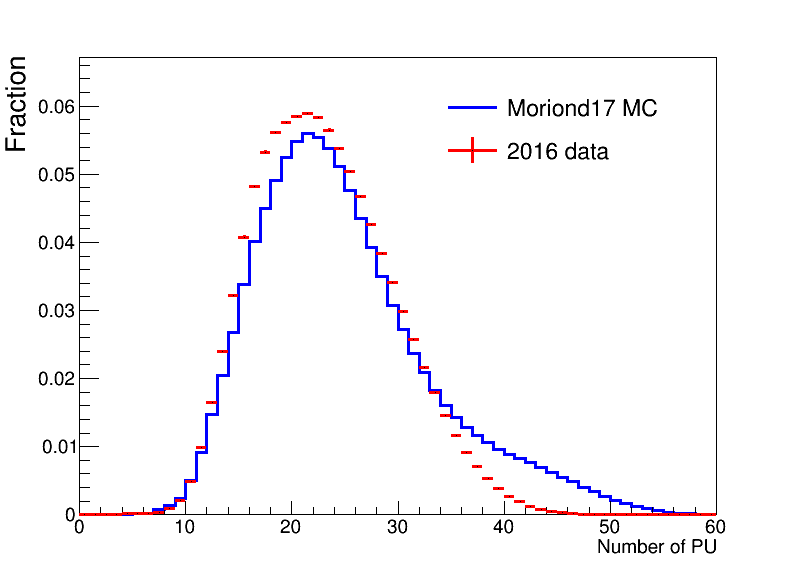
\includegraphics[width=0.45\textwidth]{figures/Zprime/PU.png}
    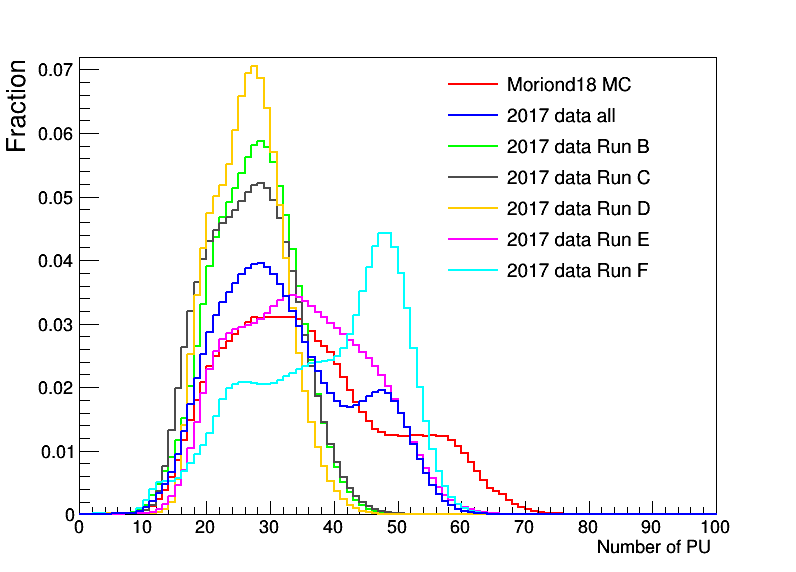
\includegraphics[width=0.45\textwidth]{figures/Zprime/2017_PU.png}
\caption{Pileup distribution for data and MC samples in 2016 (left) and in 2017 (right) .
 \label{fig:Z_pileup}}
\end{figure}

In order to improve data-mc agreement, in 2016 the data energy scale has been corrected by 1.0012 in the barrel and 1.0089 in the endcap using the mean values of the official EGamma scale corrections (except in Section \ref{sec:mass_res} study which we measured the mean data energy correction and found it agree with offical EGamma value). In 2017 the official EGamma energy scale in data and energy smearing in MC is applied in all studies.



\section{Trigger}\label{sec:Zprime_trigger}
The primary high level trigger (HLT) used in main analysis for 2016 and 2017 is HLT\_DoubleEle33\_CaloIdL\_MW which requires two electron candidates with $E_{T}$ of the supercluster higher than 33 GeV and passing loose calorimeter identification (CaloIdL) requirements and Medium Window (MW) matching between the gaussian sum filter (gsf) \cite{0954-3899-31-9-N01} track and the hits in pixel detector. In the run period of 276453 to 278822 of 2016 this trigger was prescaled and HLT\_DoubleEle33\_CaloIdL\_GsfTrkIdVL was used as the primary signal trigger. The HLT\_DoubleEle33\_CaloIdL\_GsfTrkIdVL is the same as HLT\_DoubleEle33\_CaloIdL\_MW except replacing MW pixel matching by very loose matching between gsf track and the supercluster in ECAL (GsfTrkIdVL).

The level 1 trigger (L1) seeding of the primary high level trigger is always seeded by the OR of a DoubleEG (two deposit in ECAL) seed, a SingleEG (one deposit in ECAL) seed and a SingleJet (one L1 object compatible with a jet) seed, after run 275319 in 2016 and in full 2017 it is also seeded by a SingleTau (one L1 object compatible with a $\tau$) seed. The presence of the SingleJet and SingleTau seeds are mean to mitigate the loss of efficiency for high $E_{T}$ electron. The exact unprescaled threshold of each of those seeds changing in time. The lowest threshold for the SingleEG which was always unprescaled was 40 GeV with the corresponding thresholds for the DoubleEG seed being 24 GeV,17 GeV.

The trigger efficiency will be split in L1 trigger efficiency, HLT supercluster $E_{T}$ filter efficiency (the HLT turn on curve) and online electron identification (CaloIdL+MW or GsfTrkIdVL) efficiency components. For final result only $E_{T}$ dependent efficiency will be used to weight MC events, others will be cancel in the normalisation of MC events to data in the Z peak region ($M_{ee}$ in 60-120 GeV). The method to measure the efficiency will be described in Section \ref{sec:trigger_efficiency_method}. The L1 trigger efficiency of primary signal trigger will be shown in Section \ref{sec:L1_trigger_efficiency}. The HLT $E_{T}$ turn on curve and HLT identification efficiency of primary signal trigger will be shown in Section \ref{sec:HLT_efficiency}, Other trigger efficiencies will be shown in Section \ref{sec:Other_HLT_efficiency}.

\subsection{Method for Measuring Trigger Efficiencies in Data}\label{sec:trigger_efficiency_method}
The tag and probe method \cite{CMS-AN-2009-111} is used to measure the efficiency in data. The event is selected by HLT\_Ele27\_eta2p1\_WPTight (require one HLT electron candidate with supercluster $E_{T}$ higher than 27 GeV and $|\eta|$ less than 2.1 and passing tight online electron cut) for 2016 and HLT\_Ele35\_WPTight (require one HLT electron candidate with supercluster $E_{T}$ higher than 35 GeV and passing tight online electron cut) for 2017. The tag is the electron which passing HLT\_Ele27\_eta2p1\_WPTight (HLT\_Ele35\_WPTight) in 2016 (2017) and passing HEEP ID (as defined in Section \ref{sec:Zprime_HEEP}) and in barrel of ECAL. The probe is the electron which passing the HEEP ID as well as any other requirements necessary to measure the given efficiency such as being matched to the $E_{T}$ filter to measure the trigger identification efficiency.

To simplify the computation, tags can not be probes. In the case of the probe being in the barrel, the tag is required to have a smaller supercluster $\phi$ than the probe for even number events and a larger supercluster $\phi$ for odd number events. As the sample is already very pure given there are two electrons passing HEEP ID, no background subtraction is applied, nor any mass window cut imposed. When measuring efficiencies involving the unseeded leg of the HLT\_DoubleEle33\_CaloIdL\_MW (or HLT\_DoubleEle33\_CaloIdL\_GsfTrkIdVL) trigger path, the tag should additionally pass the L1 seeded leg of that trigger and be matched to a L1 EG object, using a $\Delta R$ cone of 0.1 to be completely sure that the unseeded leg is unbiased by L1 seeded trigger. The efficiency is equal to the number of passing probes divided by all probes shown in \ref{eq:tag_probe_eff}.
\begin{equation}
\epsilon=\frac{N_{passing~probes}}{N_{all~probes}}
\label{eq:tag_probe_eff}
\end{equation}

The L1 trigger efficiency and HLT turn on curves are fitted with either a single or double turn on function (defined in terms of 'error function' $erf$). The double turn on function is shown in equation \ref{eq:turn_on}, with the single turn on function being identical except that the B terms are removed. The A0 and B0 parameters can be interpreted as the efficiency at the plateau, the A1 and B1 as the value where the efficiency reaches half maximum and A2 and B2 are the turn on of the curve.
\begin{equation}
f(E_{T})=0.5\cdot A0\cdot(1+erf(\frac{E_{T}-A1}{\sqrt{2}\cdot A2}))+0.5\cdot B0\cdot(1+erf(\frac{E_{T}-B1}{\sqrt{2}\cdot B2}))
\label{eq:turn_on}
\end{equation}

\subsection{Primary Signal Trigger: L1 Efficiency}\label{sec:L1_trigger_efficiency}
In 2016 the efficiency for a HEEP electron to pass the lowest unprescaled L1 SingleEG seed is shown in Figure \ref{fig:L1_eff_2016}. From applying to MC events, this translates to an efficiency of 99.5\% to select barrel-barrel and 98.8\% to select barrel-endcap events in a mass range of 60 to 120 GeV and a $\sim$100\% efficiency above 120 GeV. This is a lower bound on the efficiency, because there is the DoubleEG L1 seed which will further increase the efficiency. So it can be assumed the L1 seed trigger efficiency is 100\% with a 0.5\% uncertainty in the barrel and 1.2\% in the endcap.
\begin{figure}[h!]
\begin{center}
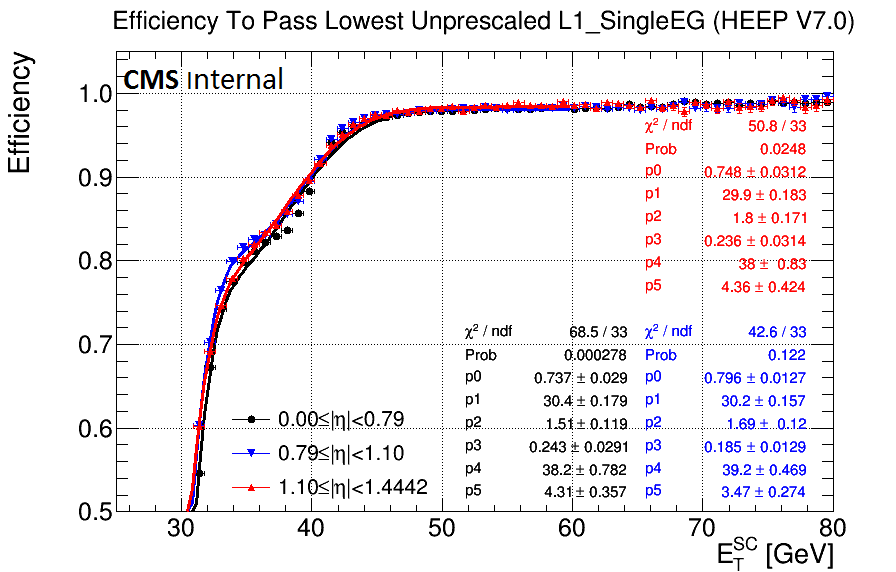
\includegraphics[width=0.45\textwidth]{figures/Zprime/2016/trigger/l1SingleEGEffEB.png}
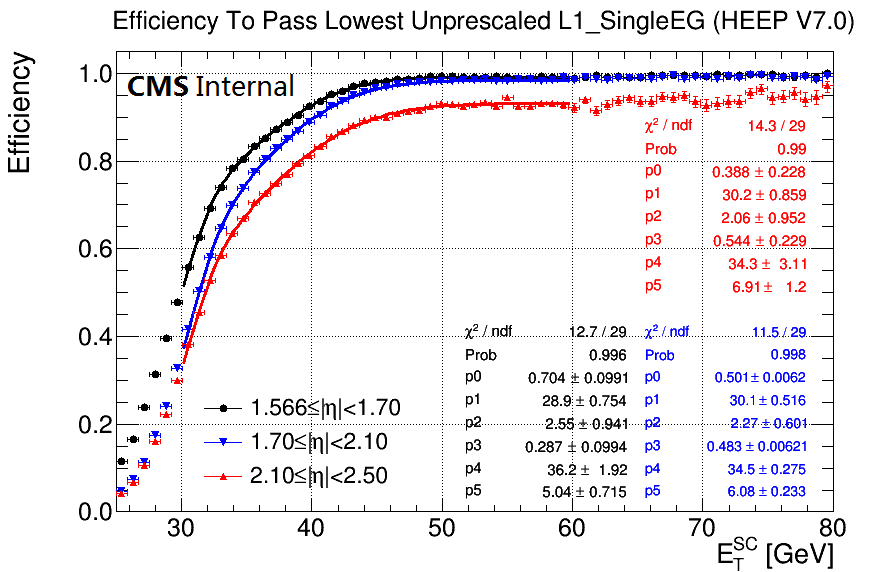
\includegraphics[width=0.45\textwidth]{figures/Zprime/2016/trigger/l1SingleEGEffEE.png}
\caption{The efficiency for an electron passing HEEP to pass the lowest unprescaled L1 SingleEG seed versus supercluster $E_{T}$ and $\eta$ in barrel (left) and in endcap (right) for 2016 \cite{CMS-AN-2016-404}.}
\label{fig:L1_eff_2016}
\end{center}
\end{figure}

In 2017 the efficiency for a HEEP electron to pass the lowest unprescaled L1 SingleEG seed is shown in Figure \ref{fig:L1_eff_2017}. In both barrel and endcap, a slow threshold related turn on and a slow general increase in efficiency in the plateau due to increasing efficiency of the L1 ID requirements are observed. From applying to MC events, this translates to an efficiency of 71\% to select barrel-barrel and 67\% to select barrel-endcap events with the worst case where the supercluster $E_{T}$ of both electrons is 35 GeV. The efficiency is higher than 99.5\% for two electrons with supercluster $E_{T}$ more than 42 GeV in barrel and more than 47 GeV in endcap. This is a lower bound on the efficiency, becasue there is the DoubleEG L1 seed which will further increase the efficiency.
\begin{figure}[h!]
\begin{center}
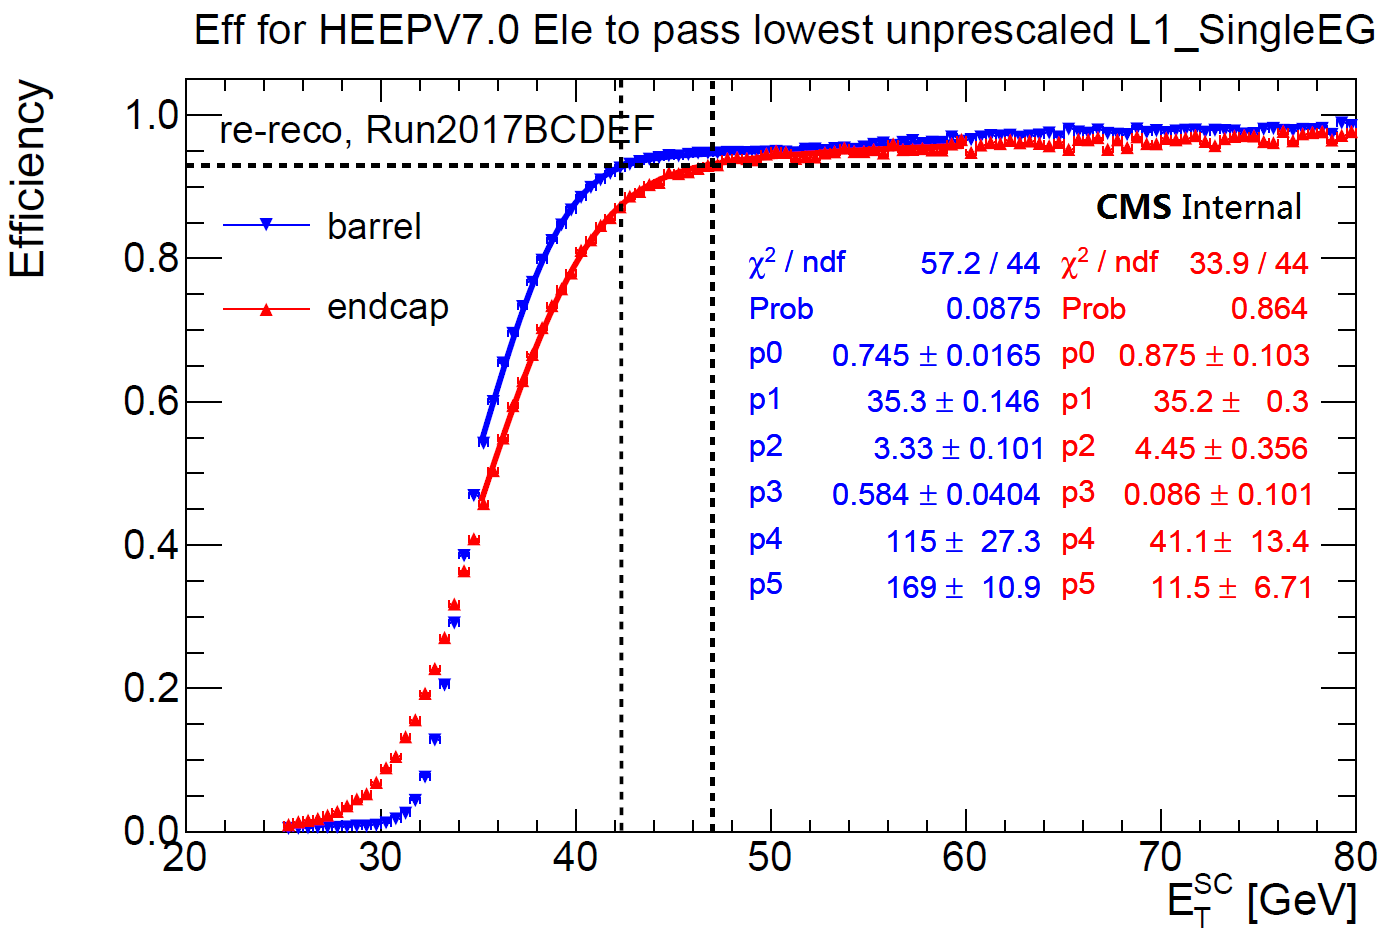
\includegraphics[width=0.5\textwidth]{figures/Zprime/2017/trigger/l1SingleEGEff.png}
\caption{The efficiency for an electron passing HEEP to pass the lowest unprescaled L1 SingleEG seed versus supercluster $E_{T}$ and $\eta$ in barrel and endcap for 2017 \cite{CMS-AN-2018-021}.}
\label{fig:L1_eff_2017}
\end{center}
\end{figure}

Due to the fact that the L1 efficiency is not 100\% for low $E_{T}$ electrons in 2017, the L1 seeded trigger turn on is considered in the 2017 analysis as described below. In data, we require for at least one of the selected electrons to be matched with the object of L1 seed trigger filter of the HLT\_DoubleEle33\_CaloIdL\_MW and with that object having a L1 $E_{T}$ greater than the lowest unprescaled L1 SingleEG seed $E_{T}$ threshold. Therefore, only L1 SingleEG seed turn on shown in Figure \ref{fig:L1_eff_2017} is used to weight MC events. Since only one electron is seeded by L1 in HLT\_DoubleEle33\_CaloIdL\_MW, the L1 weight value of selected MC events are shown in equation \ref{eq:L1_turn_on} where $P_{1}$ and $P_{2}$ are the L1 SingleEG efficiencies (shown in Figure \ref{fig:L1_eff_2017}) for leading and sub-leading selected HEEP electrons.
\begin{equation}
weight(L1)=1-(1-P_{1})\cdot(1-P_{2})=P_{1}+P_{2}-P_{1}P_{2}
\label{eq:L1_turn_on}
\end{equation}


\subsection{Primary Signal Trigger:HLT Efficiency}\label{sec:HLT_efficiency}
The HLT efficiency is divided into two components, the efficiency of the supercluster $E_{T}>33$ GeV cut (the turn on curve) and the efficiency of the CaloIdL plus MW matching (or GsfTrkIdVL) identification requirements. The turn on curves of the $E_{T}$ cut for 2016 and 2017 are shown in Figure \ref{fig:HLT_turnon_2016} and Figure \ref{fig:HLT_turnon_2017} respectively. These turn on curves are used to weight the MC events.
The efficiency of the CaloIdL plus MW matching (or GsfTrkIdVL) identification requirements for 2016 and 2017 are shown in Figure \ref{fig:HLT_ID_2016} and Figure \ref{fig:HLT_ID_2017} respectively. As the efficiencies are flat versus $E_{T}$, there is no need to weight MC events with this factor as it will automatically be included in the Z peak normalisation.

\begin{figure}[h!]
\begin{center}
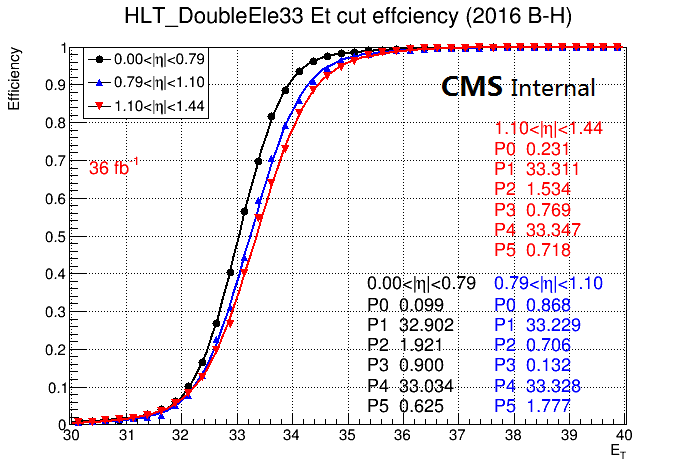
\includegraphics[width=0.45\textwidth]{figures/Zprime/2016/trigger/turnOnEEUnseeded.png}
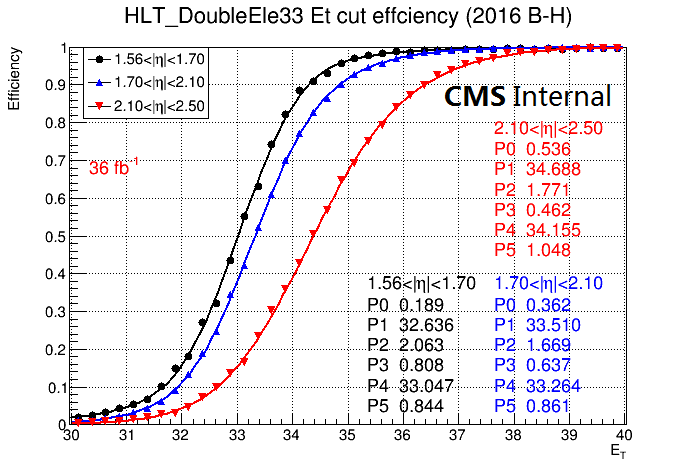
\includegraphics[width=0.45\textwidth]{figures/Zprime/2016/trigger/turnOnEBUnseeded.png}
\caption{The efficiency for electron in the barrel (left) and endcap (right) passing HEEP to pass an online supercluster $E_{T}$ > 33 GeV cut for 2016 \cite{CMS-AN-2016-404}.}
\label{fig:HLT_turnon_2016}
\end{center}
\end{figure}

\begin{figure}[h!]
\begin{center}
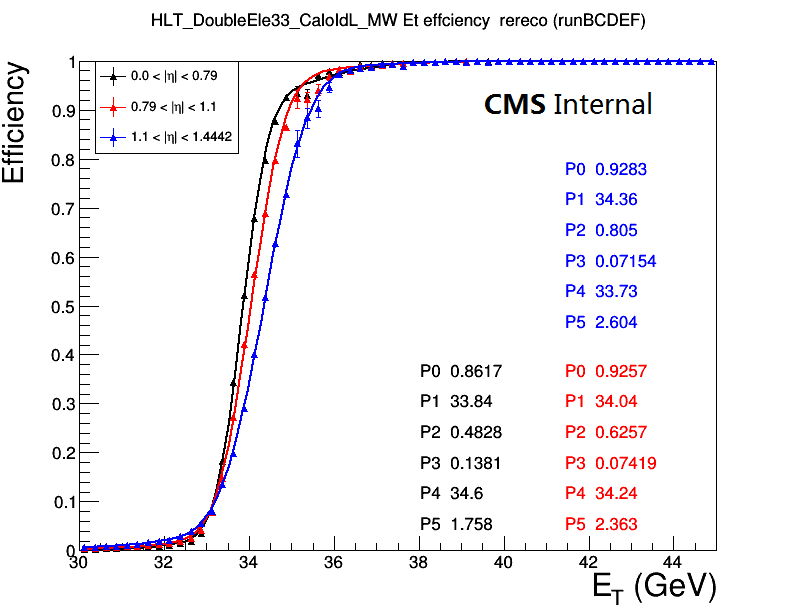
\includegraphics[width=0.45\textwidth]{figures/Zprime/2017/trigger/eff_DouEle33_Et_barrel.png}
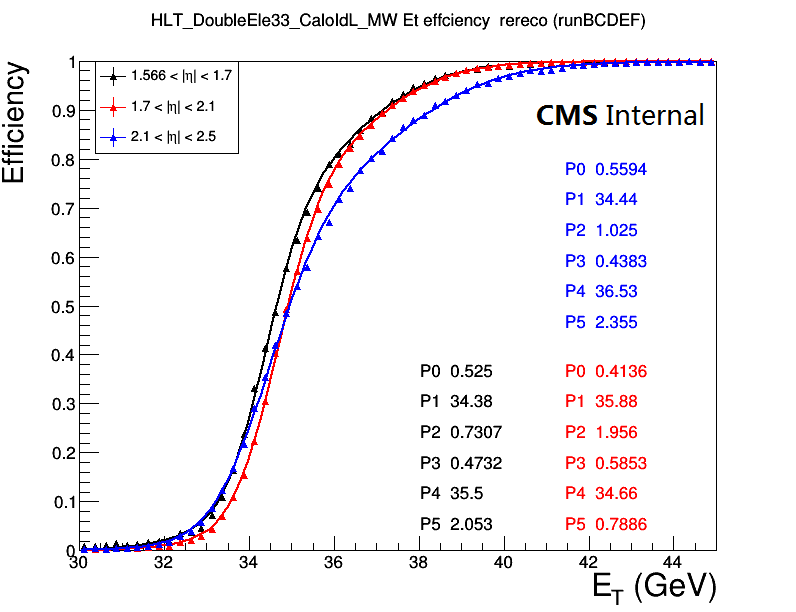
\includegraphics[width=0.45\textwidth]{figures/Zprime/2017/trigger/eff_DouEle33_Et_endcap.png}
\caption{The efficiency for electron in the barrel (left) and endcap (right) passing HEEP to pass an online supercluster $E_{T}$ > 33 GeV cut for 2017 \cite{CMS-AN-2018-021}.}
\label{fig:HLT_turnon_2017}
\end{center}
\end{figure}

\begin{figure}[h!]
\begin{center}
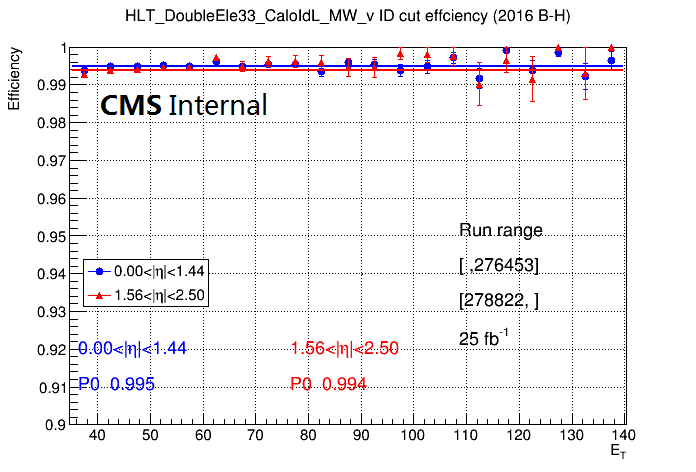
\includegraphics[width=0.45\textwidth]{figures/Zprime/2016/trigger/effMW1_DoubleEle33_SingleElectron_ID_matchedMethod.png}
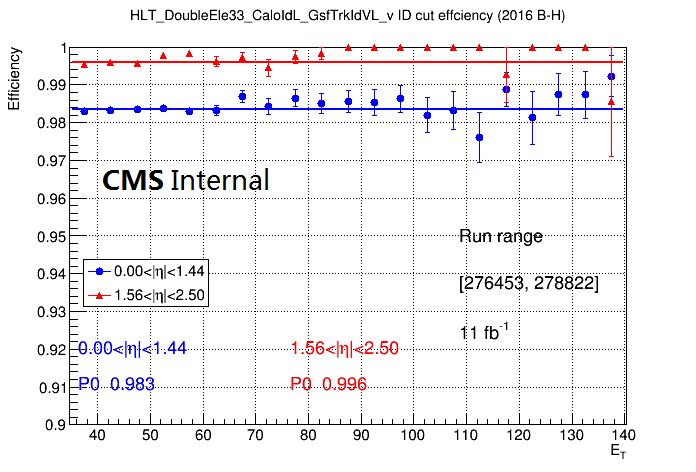
\includegraphics[width=0.45\textwidth]{figures/Zprime/2016/trigger/eff1_DoubleEle33_SingleElectron_ID_matchedMethod.png}
\caption{The efficiency for electron in the barrel and endcaps passing HEEP to pass the CaloIdL+MW ID requirement(left) and CaloIdL+GsfTrkIdVL ID requirement (right) for 2016 \cite{CMS-AN-2016-404}.}
\label{fig:HLT_ID_2016}
\end{center}
\end{figure}

\begin{figure}[h!]
\begin{center}
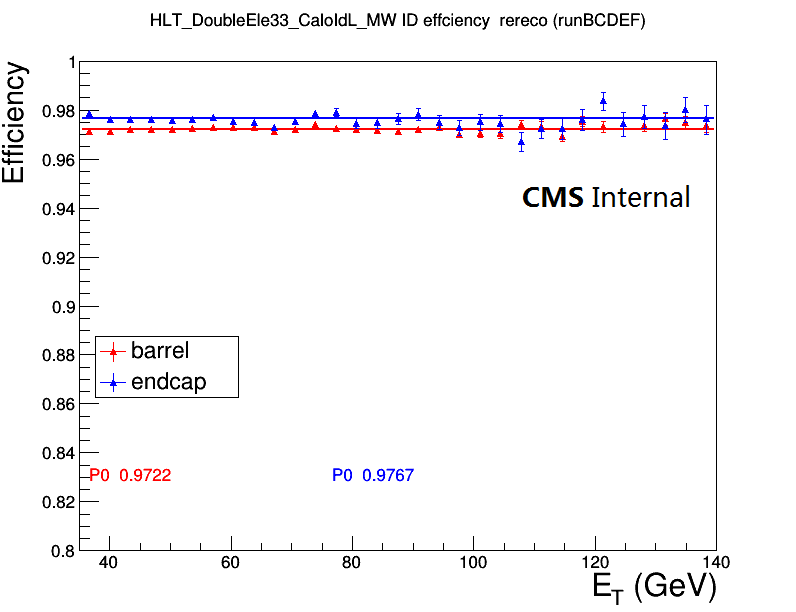
\includegraphics[width=0.5\textwidth]{figures/Zprime/2017/trigger/eff_DouEle33_ID.png}
\caption{The efficiency for electron in the barrel and endcaps passing HEEP to pass the CaloIdL+MW ID requirement for 2017 \cite{CMS-AN-2018-021}.}
\label{fig:HLT_ID_2017}
\end{center}
\end{figure}

\subsection{Other Trigger Efficiencies}\label{sec:Other_HLT_efficiency}
In 2016 the data-MC HEEP ID efficiency scale factor study uses events selected by the \\
HLT\_Ele27\_eta2p1\_WPTight trigger path. The efficiency of this path in data is shown in Figure \ref{fig:Ele27_2016}. Similar for 2017 the HLT\_Ele35\_WPTight trigger path is used and the efficiency of this trigger is shown in Figure \ref{fig:Ele35_2017}. These curves are used to weight MC events to simulate the effect of the trigger requirement in data.

\begin{figure}[h!]
\begin{center}
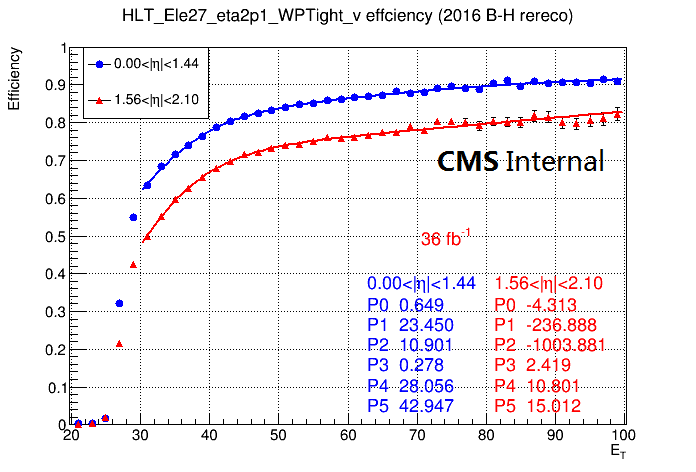
\includegraphics[width=0.5\textwidth]{figures/Zprime/2016/trigger/ele27Eff.png}
\caption{The efficiency for an electron passing HEEP to pass the HLT\_Ele27\_eta2p1\_WPTight trigger for 2016 \cite{CMS-AN-2016-404}.}
\label{fig:Ele27_2016}
\end{center}
\end{figure}

\begin{figure}[h!]
\begin{center}
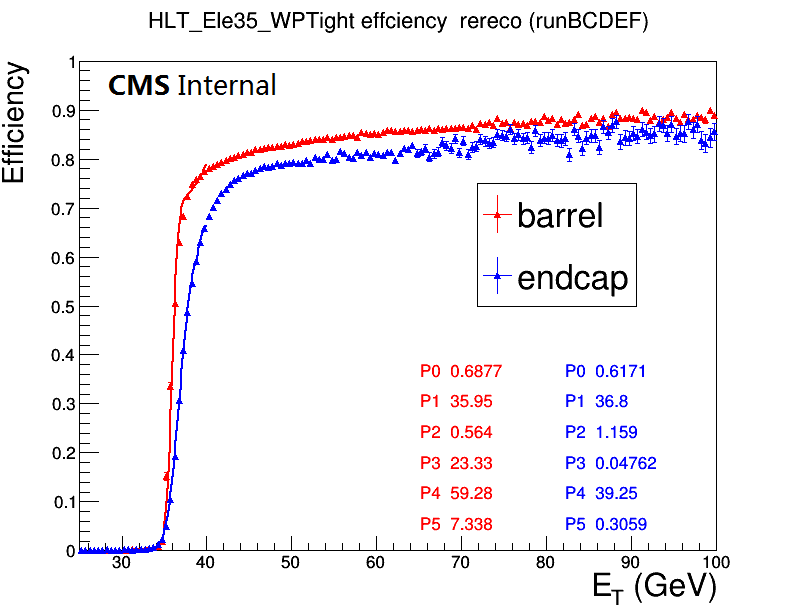
\includegraphics[width=0.45\textwidth]{figures/Zprime/2017/trigger/eff_Ele35_part1.png}
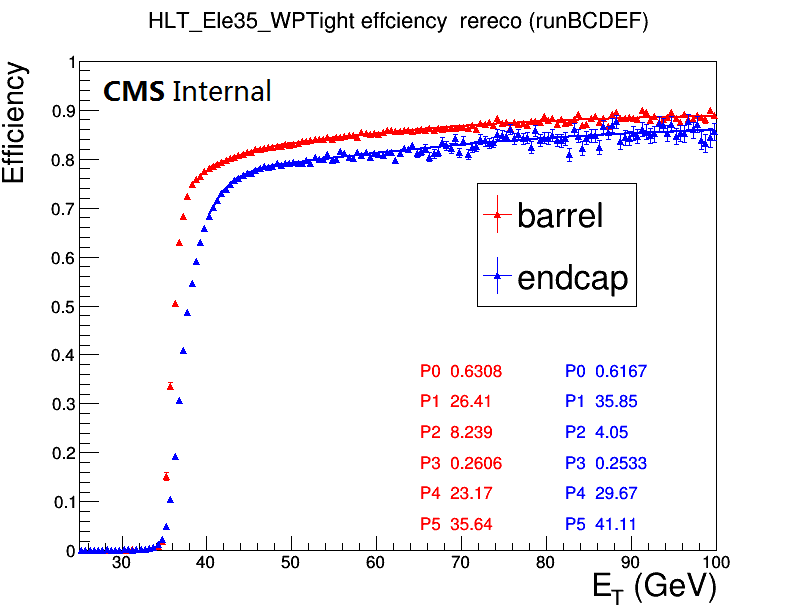
\includegraphics[width=0.45\textwidth]{figures/Zprime/2017/trigger/eff_Ele35_part2.png}
\caption{The efficiency for an electron passing HEEP to pass the HLT\_Ele35\_WPTight for $E_{T}$ less than 40 GeV (left) and $E_{T}$ more than 40 GeV (right) for 2017 \cite{CMS-AN-2018-021}.}
\label{fig:Ele35_2017}
\end{center}
\end{figure}

\section{Object and Event Selection}\label{sec:Zprime_HEEP}
Electron candidates are required to pass the so called ``HEEP'' (High Energy Electron Pairs) selection which is listed in Table \ref{tab:HEEPV70} followed by variables definition. In order to obtain well reconstructed electron candidates in tracker and ECAL sensitive regions, the candidates in the ECAL transition region (1.4442 < $|\eta|$ < 1.566) and beyond the $\eta$ coverage ($|\eta|$ > 2.5) of the tracker are therefore discarded.
After passing the HEEP selection the electrons are combined to form dielectron candidates.
If more than one dielectron candidate is found in the event, only the pair with the two largest electron \et is retained.
In addition, no charge requirement for dielectron candidates is asked and this is made to avoid efficiency losses at high mass for the main analysis.
Besides, at least one of the electron candidates has to be in barrel (events with both electron candidates in endcaps regions are rejected).
Events in data are required to satisfy the trigger selection described in Section \ref{sec:Zprime_trigger}.
MC events are weighted using turn on curves shown in Figures \ref{fig:L1_eff_2017}, \ref{fig:HLT_turnon_2016} and \ref{fig:HLT_turnon_2017} for considering the L1 and HLT effects.


\begin{table}[!h]
  \begin{center}
\smallskip\noindent
\resizebox{\linewidth}{!}{%
    \begin{tabular}{lll}
      \hline
      Variable                          & Barrel                             & Endcap                             \\
      \hline
      \multicolumn{3}{c}{Acceptance selections}\\
      \et                            & \et$>$ 35 GeV                    & \et$>$ 35 GeV                    \\
      $\eta$                            & $|\eta| < 1.4442$             & $1.566 < |\eta| < 2.5$        \\
      \hline
      \multicolumn{3}{c}{Identification selections}\\
      %\texttt{isEcalDriven}             & true                               & true                               \\
      $\Delta\eta_{in}^{seed}$          & $|\Delta\eta_{in}^{seed}| < 0.004$ & $|\Delta\eta_{in}^{seed}| < 0.006$ \\
      $\Delta\phi_{in}$                 & $|\Delta\phi_{in}| < 0.06$         & $|\Delta\phi_{in}| < 0.06$         \\
      $H/E$                             & $H/E < 1/E + 0.05$                 & $H/E < 5/E + 0.05$                 \\
      $\sigma_{i\eta i\eta}$            & -                                  & $\sigma_{i\eta i\eta} < 0.03$      \\
      $\frac{\EOnexFive}{\EFive}$ and $\frac{\ETwoxFive}{\EFive}$        & $\frac{\EOnexFive}{\EFive}>0.83$ or $\frac{\ETwoxFive}{\EFive}>0.94$ & -                              \\
      Inner layer lost hits             & lost hits $\le 1$                  & lost hits $\le 1$                    \\
      Impact parameter $d_{xy}$        & $|d_{xy}|<0.02$ cm                   & $|d_{xy}|<0.05$ cm                   \\
      isEcalDriven                     & true                                  & true                                  \\
      \hline
      \multicolumn{3}{c}{Isolation selections}\\
      \small{Calorimeter isolation} $Iso$                  & $Iso < 2 + 0.03\et[\mathrm{GeV}] + 0.28\rho$     & $Iso < 2.5 + 0.28\rho$ (\et<50 GeV) \\
                                        &                                    & else $Iso < 2.5 + 0.03(\et[\mathrm{GeV}]-50) + 0.28\rho$ \\
      Track \pt isolation $Isopt$       & $Isopt <$ 5 GeV                   & $Isopt <$ 5 GeV                   \\
      \hline
    \end{tabular}}
    \caption{The definitions of HEEP selection cuts \cite{HEEP_twiki}.}
    \label{tab:HEEPV70}
  \end{center}
\end{table}

The variables used in the HEEP definition are defined as follows \cite{HEEP_twiki}:
\begin{itemize}
\item[$\bullet$] \textbf{$\Delta\eta_{in}^{seed}$}:
 it is the difference in $\eta$ between the track position as measured in the inner layers, extrapolated to the interaction vertex and then extrapolated to the calorimeter and the $\eta$ of the supercluster's seed. The cut value in the barrel (0.004) is tighter than in the endcaps (0.006), because the tracker material budget is thicker in the endcaps and it reduces the precision on the position measurement.
\item[$\bullet$] \textbf{$\Delta\phi_{in}$}: it is the difference in $\phi$ between the track position as measured in the inner layers, extrapolated to the interaction vertex and then extrapolated to the calorimeter and the $\phi$ of the supercluster. Since there is a wider spread of the energy in $\phi$ with respect to $\eta$ due to photon emissions from bremsstrahlung processes of a electron, the distribution of $\Delta\phi_{in}$ is much broader than $\Delta\eta_{in}^{seed}$. Hence, The cut value of $\Delta\phi_{in}$ (0.06 in both barrel and endcap regions) is around ten times looser than for $\Delta\eta_{in}^{seed}$.

\item[$\bullet$] \textbf{\hoe}: it is a ratio of hadronic energy of the HCAL tower in a cone of radius 0.15 centred on the electron's position in the calorimeter to the electromagnetic energy of the electron's supercluster.

\item[$\bullet$] \textbf{\sieie}:
it is a measure of the spread in $\eta$ in units of crystals of the electrons energy in the $5\times5$ block centred on the seed crystal. It is computed as:
    $$\sieie = \sqrt{ \frac
      { \sum_{i \in 5\times5} \left( \eta_i - \bar \eta \right )^2 w_i
      } {\sum_{i \in 5\times5} w_i} }, ~~~~
    w_i = \max \left( 0, 4.7 + \log(E_i / E_{5\times5}) \right ).
    $$
\item[$\bullet$] \textbf{$\frac{\EOnexFive}{\EFive}$}: it is the ratio of the energy contained in the 1$\times$5 domino in $\eta\times\phi$ in the barrel ($x\times y$ in the endcaps) centered in $\phi$ on the seed crystal of the supercluster over the energy of the 5$\times$5 matrix centered on the same seed crystal.
\item[$\bullet$] \textbf{$\frac{\ETwoxFive}{\EFive}$}: it is the ratio of the energy contained in the most energetic 2$\times$5 domino in $\eta\times\phi$ in the barrel ($x\times y$ in the endcaps) centered in $\phi$ on the seed crystal of the supercluster over the energy of the 5$\times$5 matrix centered on the same seed crystal.
\item[$\bullet$] Inner layer lost hits : it is defined as the number of missing hits in the innermost layers of the tracker
(including the pixel) before the gsf track first hit. It is mainly designed to reject photons that convert into a pair of electrons in the tracker.
\item[$\bullet$] Impact parameter $d_{xy}$: it is the closest distance (in the transverse plane) between the primary vertex and the track of the gsf electron candidate. The distribution is wider in the endcaps due to the poorer resolution on the track momentum in that region. Similarly to the missing hit cut, the $d_{xy}$ cut is mainly useful to reject converted photons.
\item[$\bullet$] isEcalDriven : electrons can be ecal driven (found using egamma techniques) or tracker driven (found using particle flow algorithm). Tracker driven is useful for low energy electrons, while it is not useful or validated for high energy electrons. Hence we require that the electron be ecal driven.
\item[$\bullet$] ECAL isolation: it is defined as the scalar sum of the transverse energy of all the ECAL crystals with \et$>$
80 MeV in the barrel (\et$>$ 100 MeV in the endcaps) in a cone of $\Delta R$ = 0.3
centered on the gsf electron candidate position in the calorimeter, excluding those
in an inner cone of radius 3 crystals and those in a $|\eta|$ strip of total width of 3 crystals (see left side of Figure \ref{iso_pic}).
The inner cone veto removes the electron energy from the sum whereas the $|\eta|$ strip removes the energy from the bremsstrahlung photons.
\item[$\bullet$] { HCAL isolation: it is defined as the sum of transverse energy collected by all the towers
of the first layer of the HCAL in a cone of $\Delta R$ = 0.3 centered on the gsf electron
candidate position in the calorimeter, excluding the towers in a cone of $\Delta R$ = 0.15 (see right side of Figure \ref{iso_pic}).
\begin{figure}[!htbp]
\begin{center}
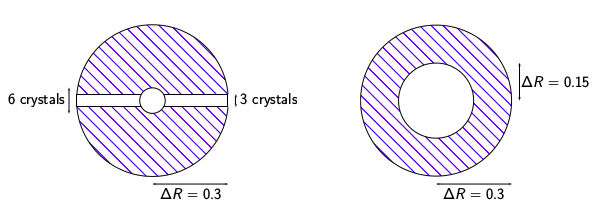
\includegraphics[width=0.8\textwidth]{figures/Zprime/iso.png}
\end{center}
\caption{Definition of the regions used to compute the ECAL (left) and HCAL (right) isolation.}
\label{iso_pic}
\end{figure}}

\item[$\bullet$] Calorimeter isolation $Iso$: it is sum of the ECAL isolation and the HCAL isolation (defined in the previous points). The variable is strongly dependent on the electron energy and tends to increase for high \et~electrons due to the extension of the shower. A cut value of the
form $Iso < a + b\cdot E_T$ is therefore applied.
\item[$\bullet$] Track \pt isolation $Isopt$: it is defined as the sum of the \pt of all the reconstructed
tracks between an inner and outer cone around the gsf electron. The $\Delta R$ for the inner cone is 0.04 and it is 0.3 for the outer cone.
Besides, only tracks having \pt > 700 MeV and $|\Delta z|$ with the gsf electron track $<$ 0.2 cm are considered, where z is the minimum distance of
the track to the nominal interaction point (0,0,0).
%The inner cone veto is present
%to remove duplicate tracks associated to the electron as well as tracks from converted
%bremsstrahlung photons. This variable substitutes the default tracker isolation variable in the gsf electron, for which the efficiency has a large pile-up dependence starting at $\et\sim100$~GeV, due to a misbehaviour of the reconstruction software that allows many low quality tracks to enter the isolation cone.  The track isolation variable has then been redefined introducing ad-hoc ``high purity'' requirements which removed most of the problematic tracks that introduced the pile-up dependance of this variable.
\end{itemize}

\section{Mass Resolution and Scale}
\label{sec:mass_res}

The mass resolution of heavy resonances is a crucial point of the analysis, since its outcome enters in the signal model definition. Its estimation follows two steps: a data-MC comparison, and a MC-only study.
The first step consists in the comparison between data and DY MC for the resolution and mean value of the invariant mass distribution of the electron pairs passing the HEEP ID at the Z peak (80 GeV $<M_{ee}<$ 100 GeV).
The distributions are fitted using a Breit-Wigner (B-W) function (whose parameters are fixed to the PDG values of the Z boson) convoluted with a double-sided crystal ball function (dCB) (which is defined as a Gaussian core connected with two power-law functions on both sides).
The $\sigma$ parameter from the dCB function is then compared between data an MC in different $\eta$-categories. For BB category both electrons are required to be in the ECAL barrel. For BE category one electron is required to be in the ECAL barrel, and the other one in one of the ECAL endcaps.
Fit results for data and MC in 2016 (2017) are shown in Figure \ref{fig:data_MC_peak_2016} (\ref{fig:data_MC_peak_2017}).

The $\sigma_{MC}$ of the dCB from the fit to the MC distribution is subtracted in quadrature by the $\sigma_{data}$ coming from the fit to the data, and defining the $\sigma_{extra}$ through the relation: $\sigma_{extra}=\sqrt{\sigma_{data}^{2} - \sigma_{MC}^{2}}$.
In Table \ref{tab:extra} the results for the $\sigma_{extra}$ are shown for the different categories for 2016 and 2017.
Note that the numbers in Table \ref{tab:extra} are presented in percentage [\%] of the Z peak mass value (it is 91.1876 GeV for $M_{Z}$ DPG ). The quoted mean values are the ones of the dCB function used to fit the mass spectra after convolution with the B-W function. For 2017 the official EGamma energy scale and smearing is applied for data and MC, therefore the mean value difference between data and MC in 2017 is much smaller than that in 2016 and for the $\sigma_{extra}$ which is 0 in 2017 because of the larger $\sigma_{MC}$ than $\sigma_{data}$.

\begin{figure}[ht]
  \begin{center}
    \begin{tabular}{cc}
      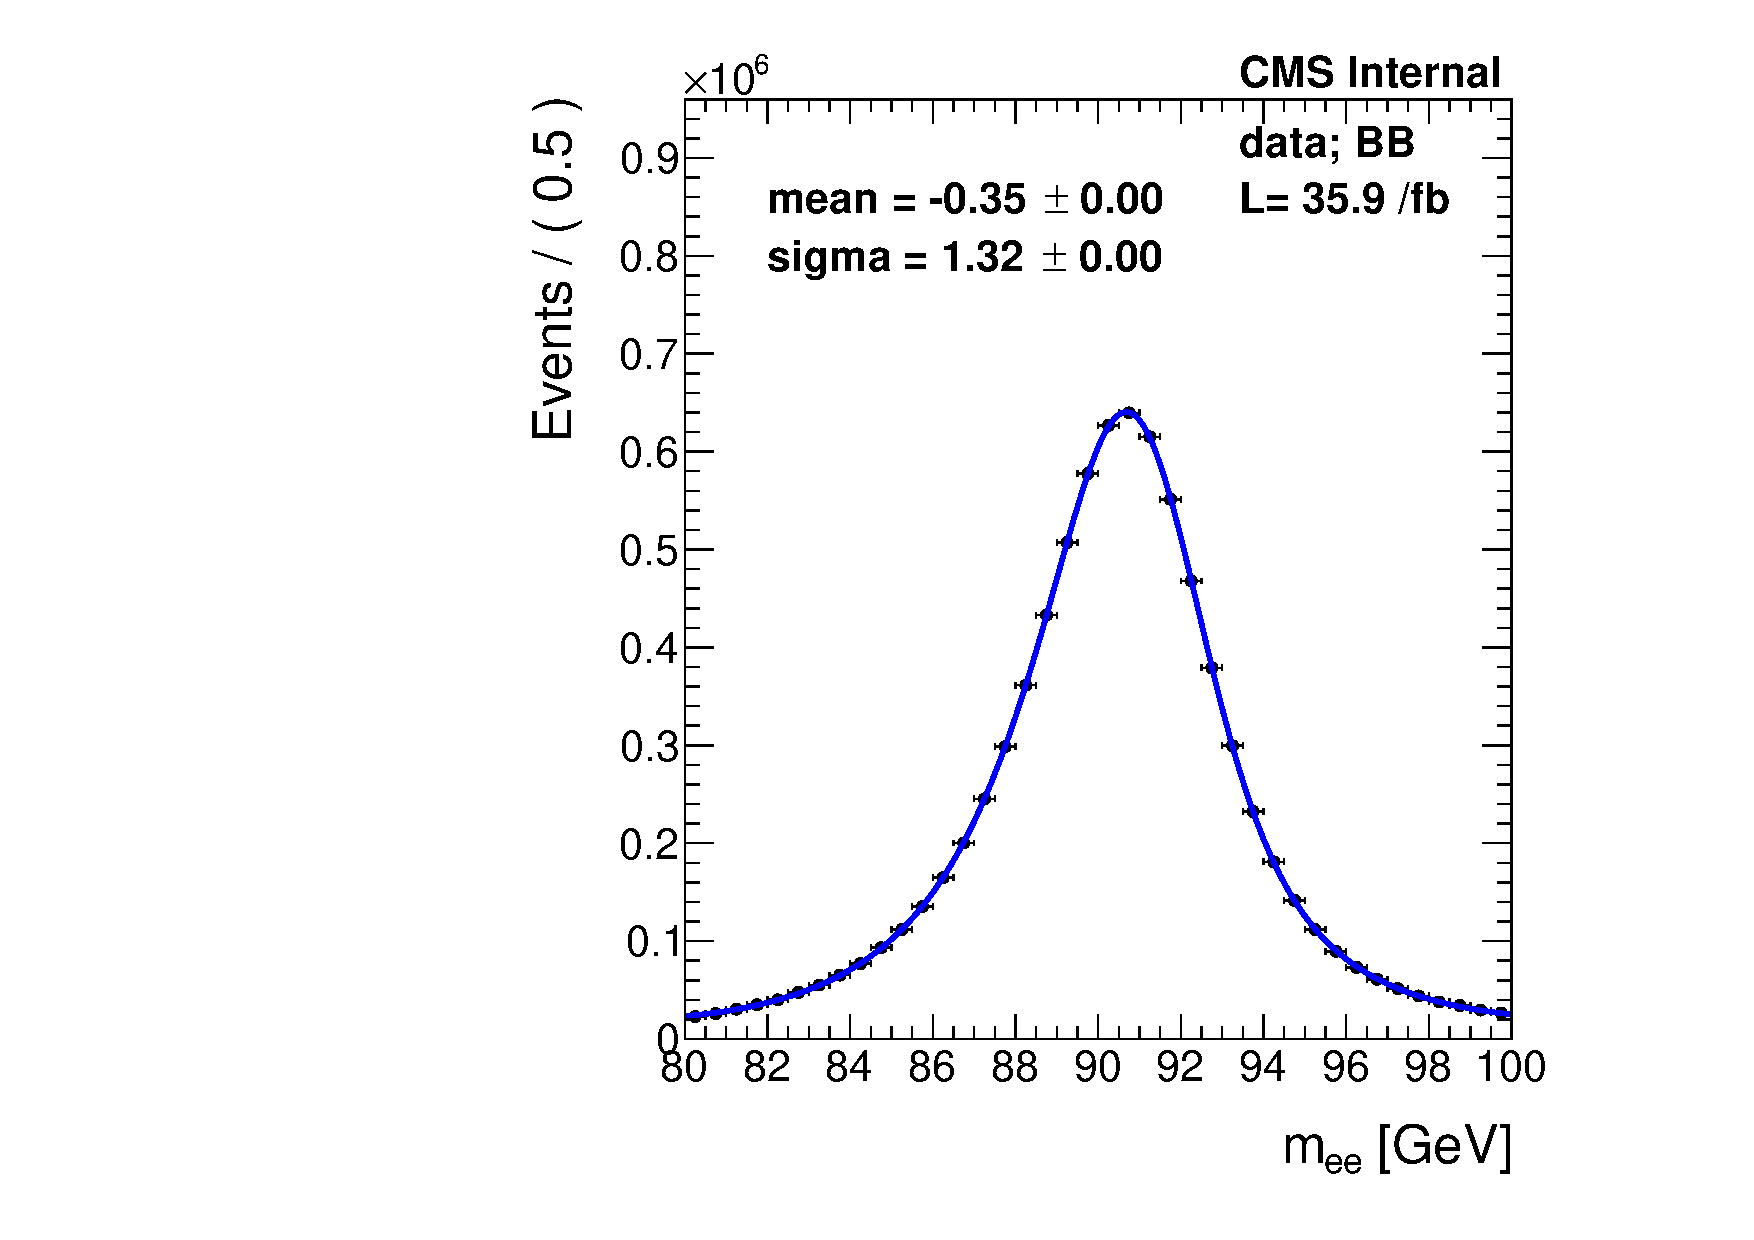
\includegraphics[width=0.48\textwidth]{figures/Zprime/2016/mass_resolution/h_mee_data_BB_2016_Moriond17.pdf} &
      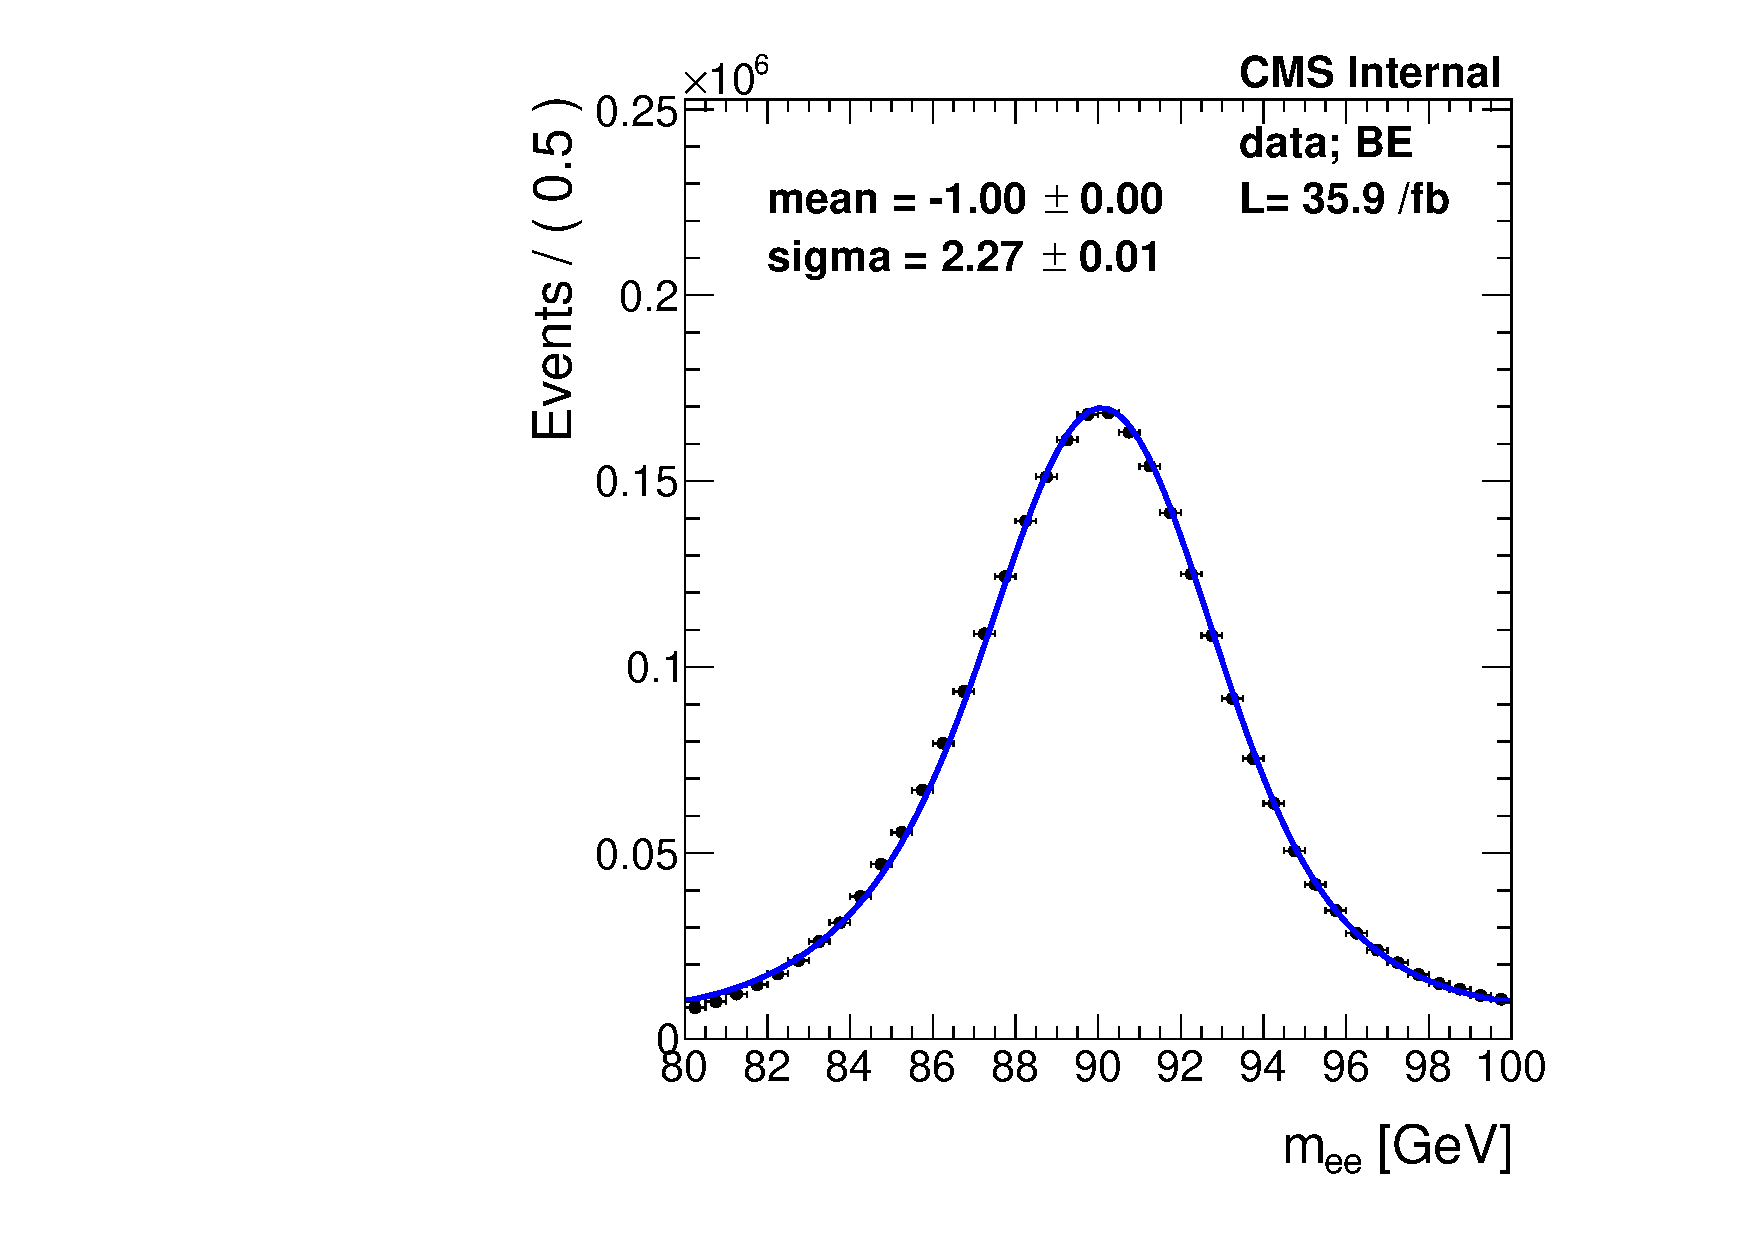
\includegraphics[width=0.48\textwidth]{figures/Zprime/2016/mass_resolution/h_mee_data_BE_2016_Moriond17.pdf} \\
      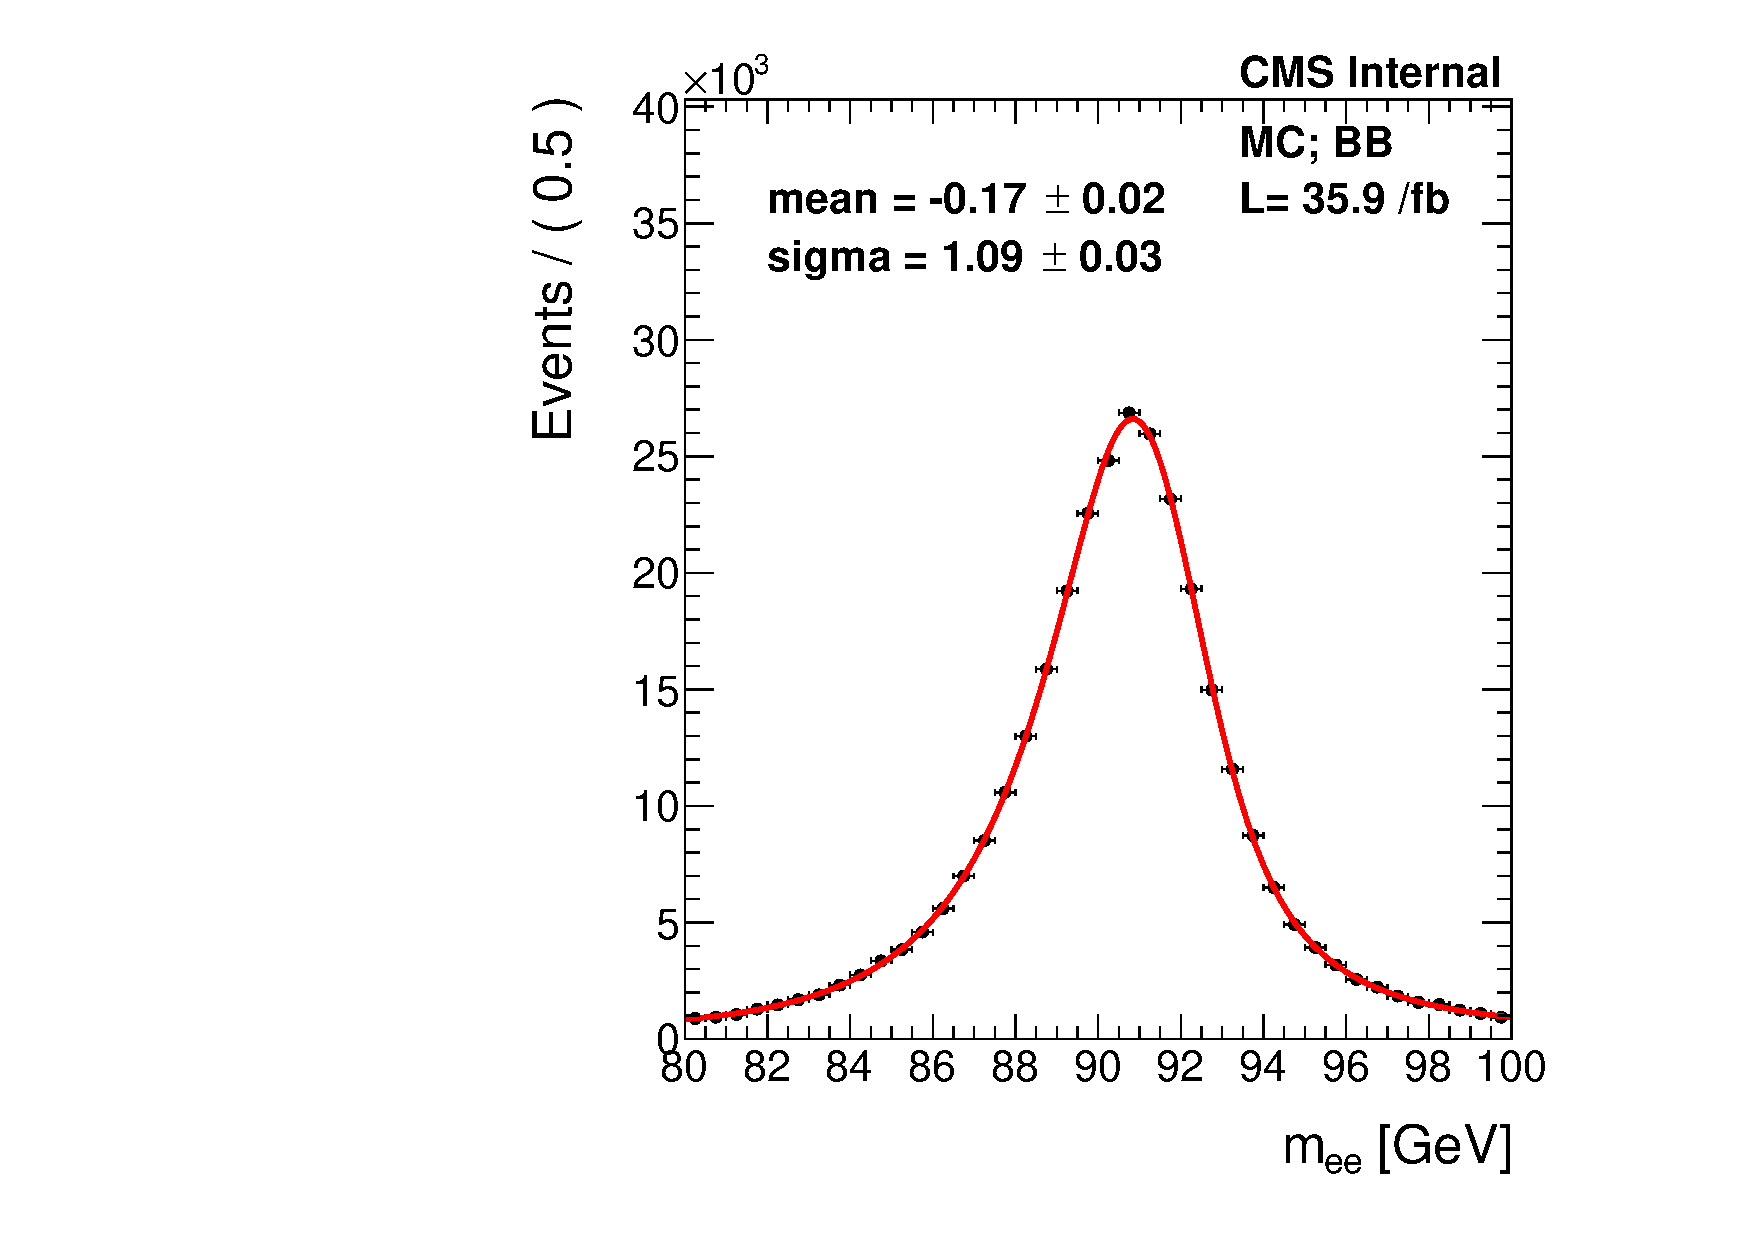
\includegraphics[width=0.48\textwidth]{figures/Zprime/2016/mass_resolution/h_mee_MC_BB_2016_Moriond17.pdf} &
      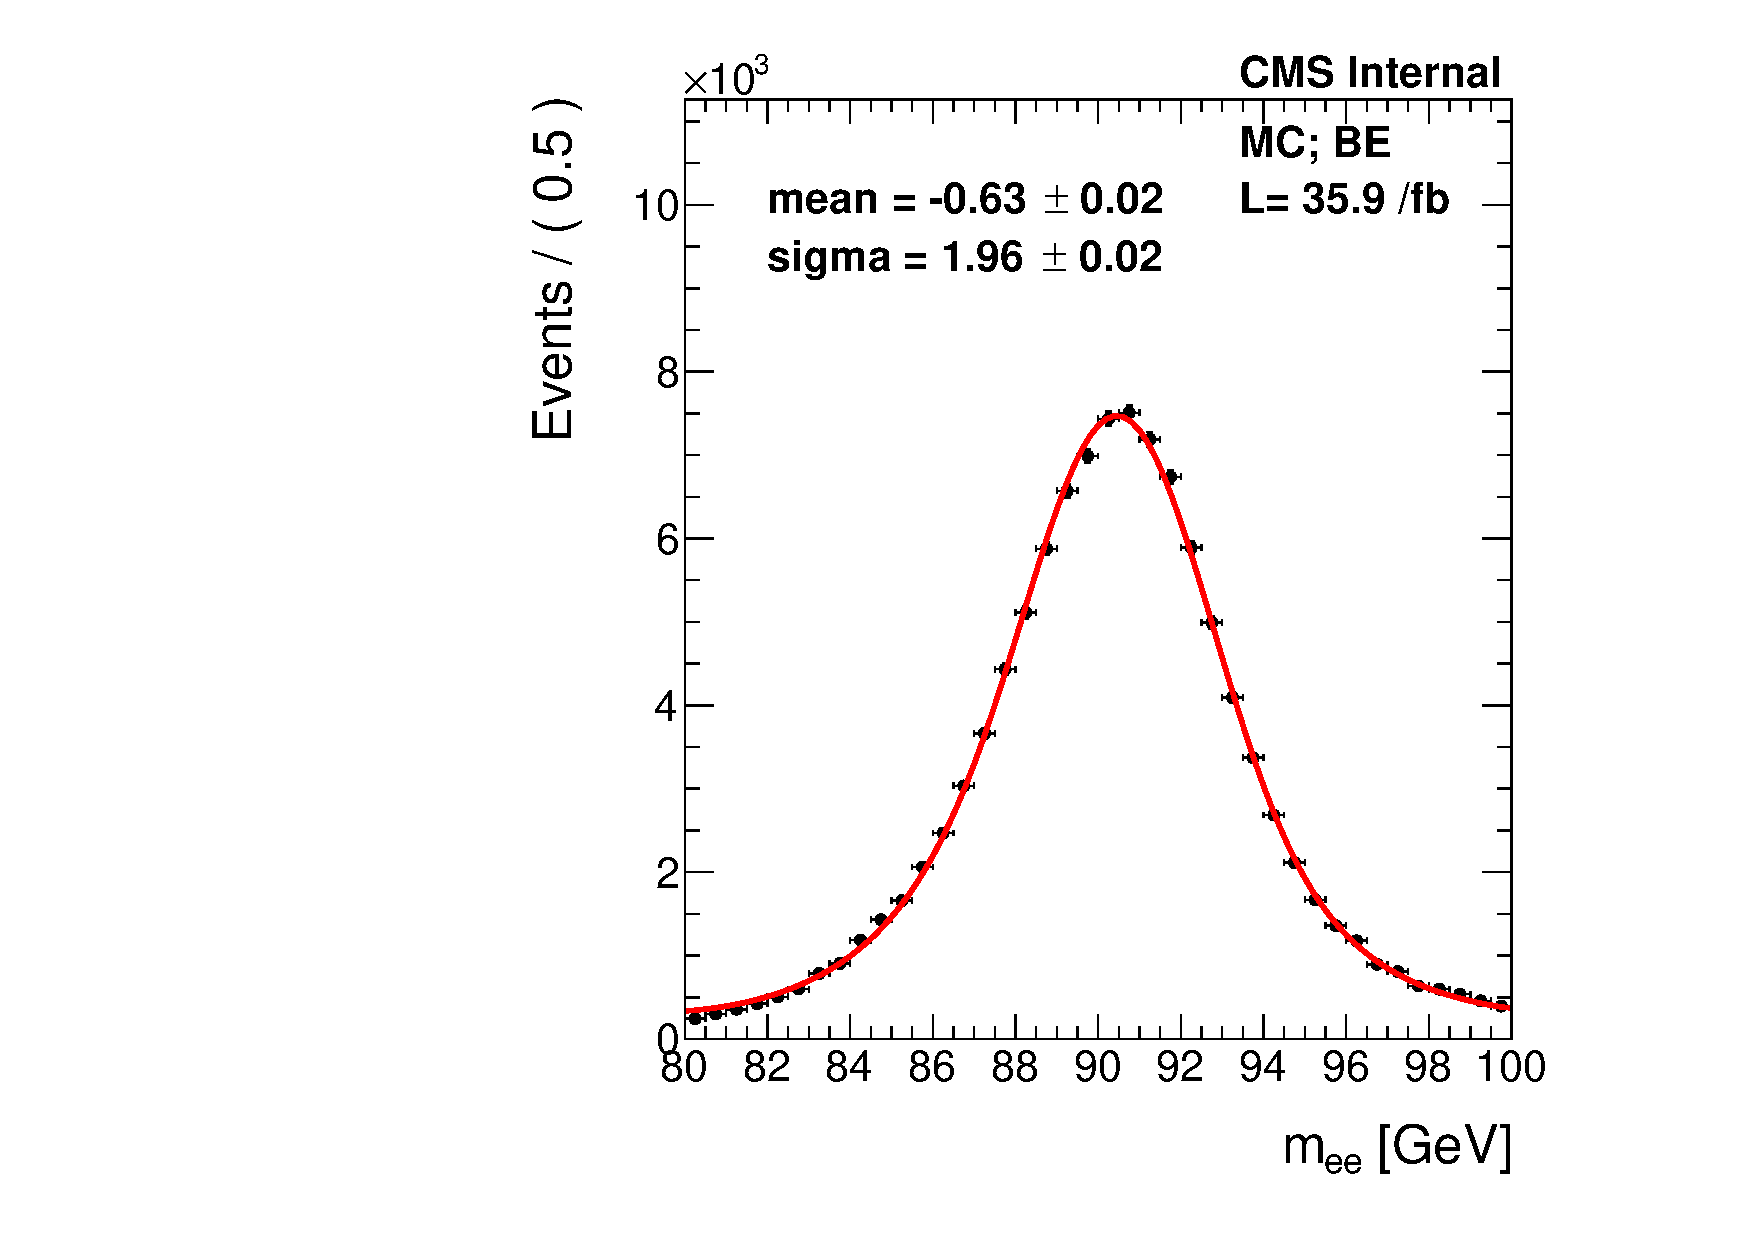
\includegraphics[width=0.48\textwidth]{figures/Zprime/2016/mass_resolution/h_mee_MC_BE_2016_Moriond17.pdf}
    \end{tabular}
    \caption{The distributions of dielectron invariant masses at the Z peak in data (top) and MC (bottom) for the BB (left) and BE (right) regions in 2016 \cite{CMS-AN-2016-404}.
    \label{fig:data_MC_peak_2016}}
  \end{center}
\end{figure}

\begin{figure}[ht]
  \begin{center}
    \begin{tabular}{cc}
      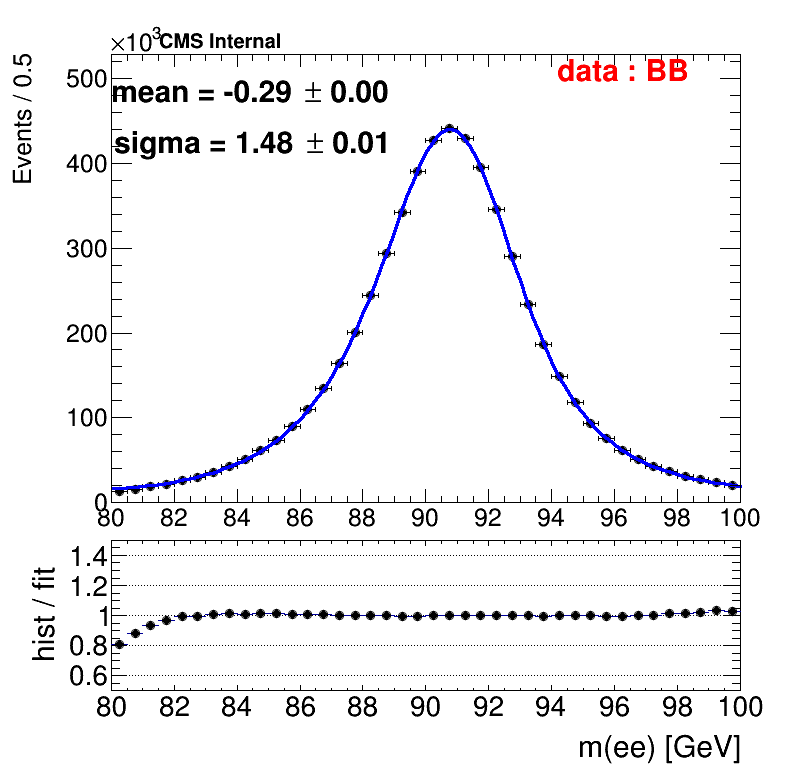
\includegraphics[width=0.48\textwidth]{figures/Zprime/2017/mass_resolution/data_BB_RunBCDEF} &
      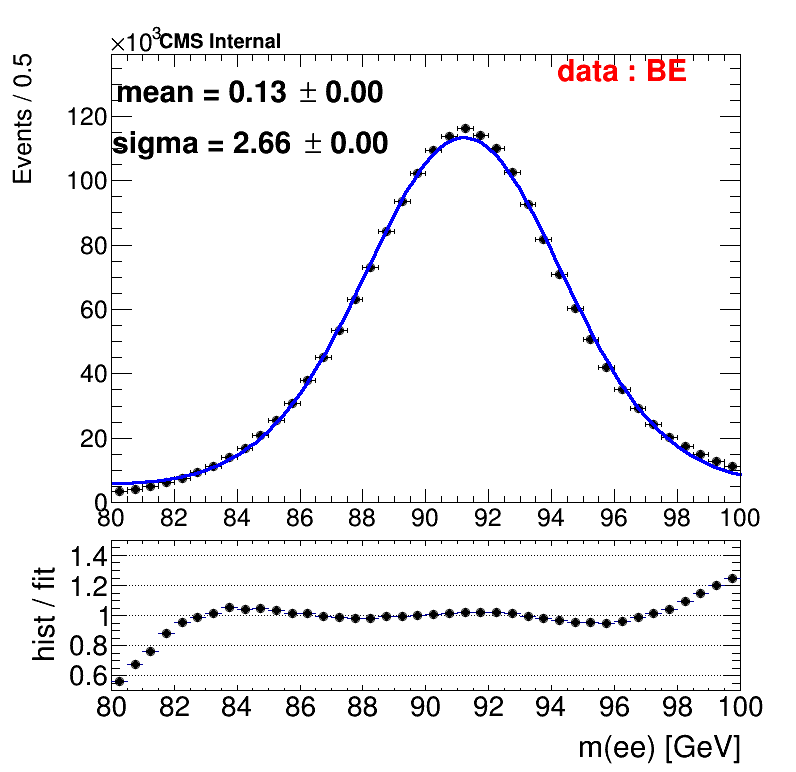
\includegraphics[width=0.48\textwidth]{figures/Zprime/2017/mass_resolution/data_BE_RunBCDEF} \\
      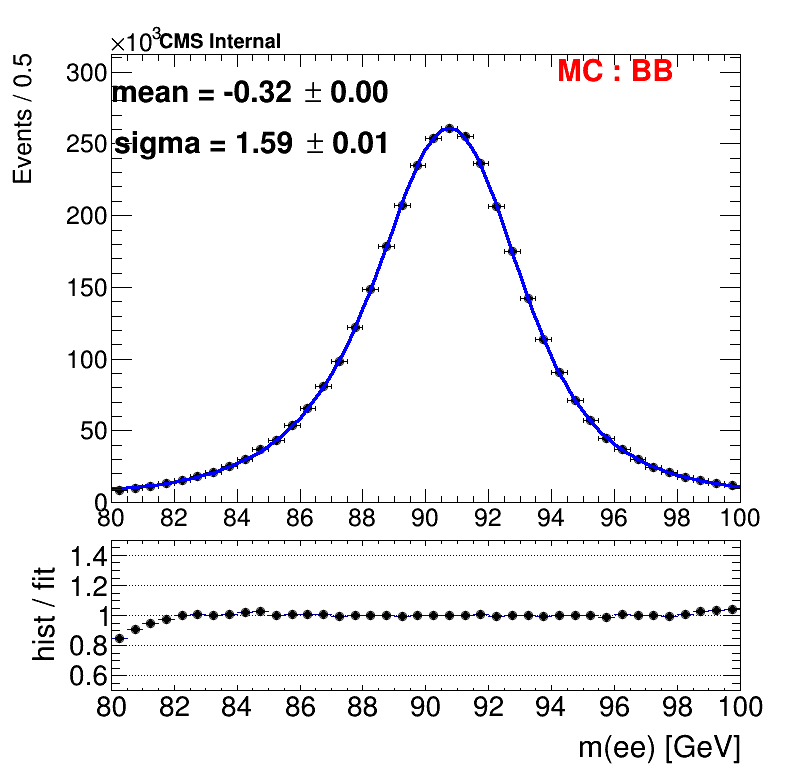
\includegraphics[width=0.48\textwidth]{figures/Zprime/2017/mass_resolution/mc_BB} &
      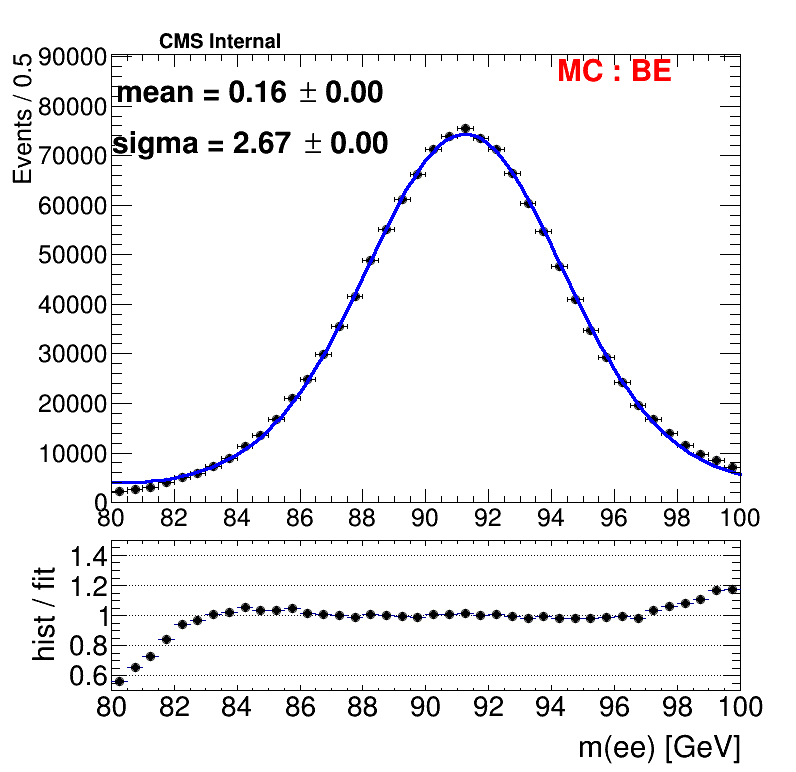
\includegraphics[width=0.48\textwidth]{figures/Zprime/2017/mass_resolution/mc_BE}
    \end{tabular}
    \caption{The distributions of dielectron invariant masses at the Z peak in data (top) and MC (bottom) for the BB (left) and BE (right) regions in 2017.
    \label{fig:data_MC_peak_2017}}
  \end{center}
\end{figure}



\begin{table}[htb]
\begin{center}
\begin{tabular}{cccccc}
\hline
Year &Category            & $\frac{\Delta M}{M} [\%]$ & $\sigma_{data}$ [\%] & $\sigma_{MC}$ [\%] & $\sigma_{extra}$ [\%] \\ \hline
\multirow{2}{*}{2016}     &BB       & -0.19 $\pm$ 0.02          & 1.45 $\pm$ 0.00      & 1.20 $\pm$ 0.03    & 0.81 $\pm$ 0.04  \\
                          &BE       & -0.40 $\pm$ 0.02          & 2.49 $\pm$ 0.01      & 2.15 $\pm$ 0.03    & 1.26 $\pm$ 0.05  \\ \hline
\multirow{2}{*}{2017}     &BB       & 0.04 $\pm$ 0.01           & 1.63 $\pm$ 0.01      & 1.74 $\pm$ 0.01    & 0 $\pm$ 0 \\
                          &BE       & -0.03 $\pm$ 0.00          & 2.91 $\pm$ 0.00      & 2.93 $\pm$ 0.00    & 0 $\pm$ 0 \\ \hline
\end{tabular}
\caption{The results of scale shift $\frac{\Delta M}{M}$  between data and MC, as well as the $\sigma_{extra}$ parameters per category. \label{tab:extra}}
\end{center}
\end{table}
\medskip


In 2017 we also checked mass scale and resolution for data and MC as a function of \et, energy and $\eta$ of electron using the method explained above.
Results are shown from Figure \ref{fig:data_MC_Et_E_BB} to \ref{fig:data_MC_eta_BB_BE}. In all \et and  $\eta$ ranges, the data and MC show good agreement.
The energy scale at high \et is validated to within 2\% for barrel electrons and 1\% for endcap elections.

\begin{figure}[ht]
  \begin{center}
    \begin{tabular}{cc}
      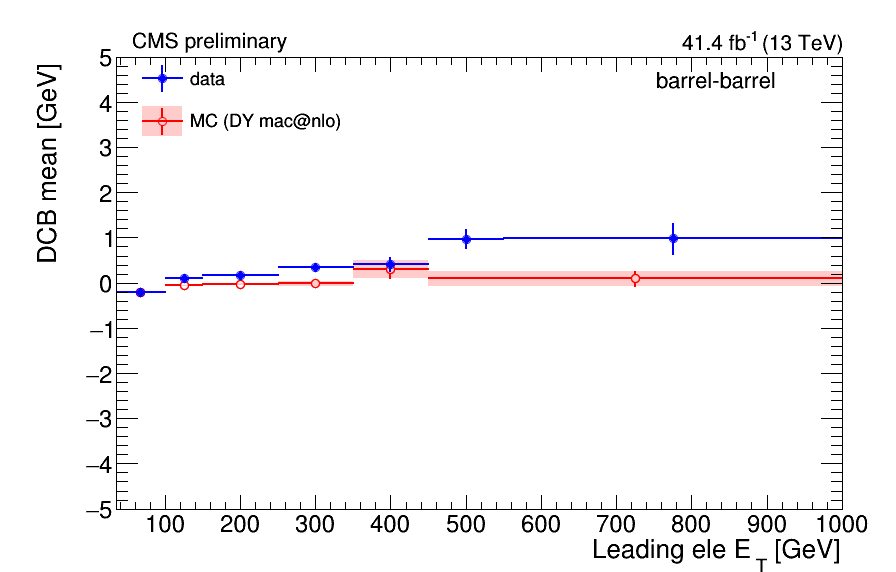
\includegraphics[width=0.48\textwidth]{figures/Zprime/2017/mass_resolution/scale_check/h_led_Et_Mee_BB_scale} &
      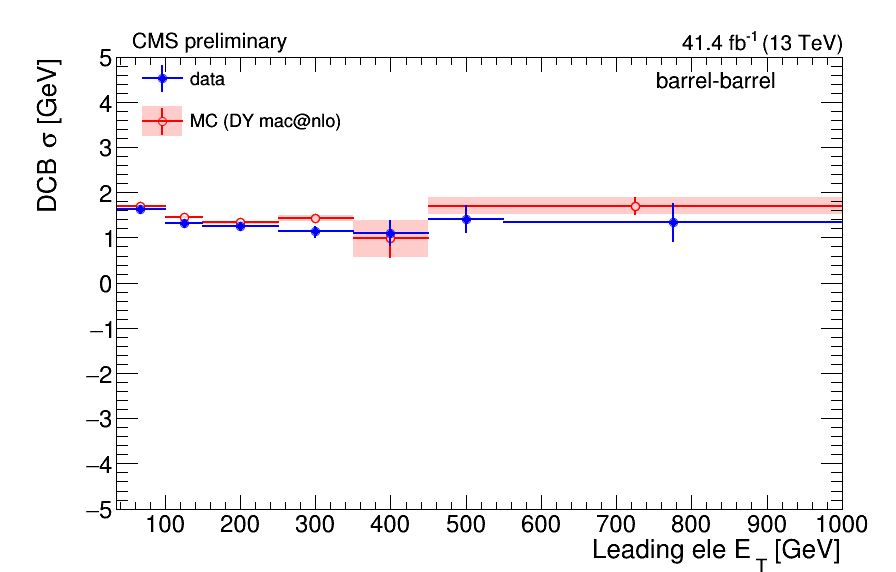
\includegraphics[width=0.48\textwidth]{figures/Zprime/2017/mass_resolution/scale_check/h_led_Et_Mee_BB_resolution} \\
      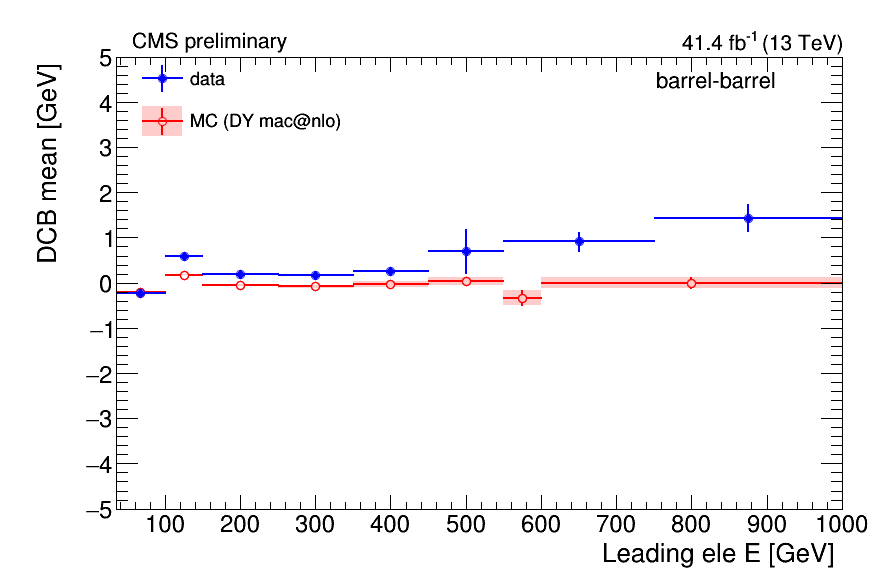
\includegraphics[width=0.48\textwidth]{figures/Zprime/2017/mass_resolution/scale_check/h_led_E_Mee_BB_scale} &
      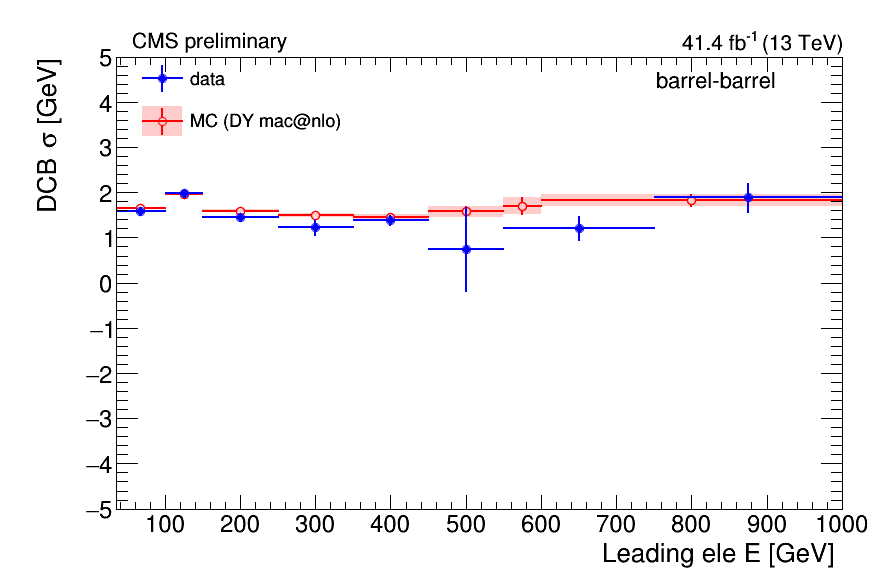
\includegraphics[width=0.48\textwidth]{figures/Zprime/2017/mass_resolution/scale_check/h_led_E_Mee_BB_resolution}
    \end{tabular}
    \caption{The mean (left) and sigma (right) values of dCB as the function of \et (top) and energy (bottom) of leading electron for barrel-barrel channel.
    \label{fig:data_MC_Et_E_BB}}
  \end{center}
\end{figure}

\begin{figure}[ht]
  \begin{center}
    \begin{tabular}{cc}
      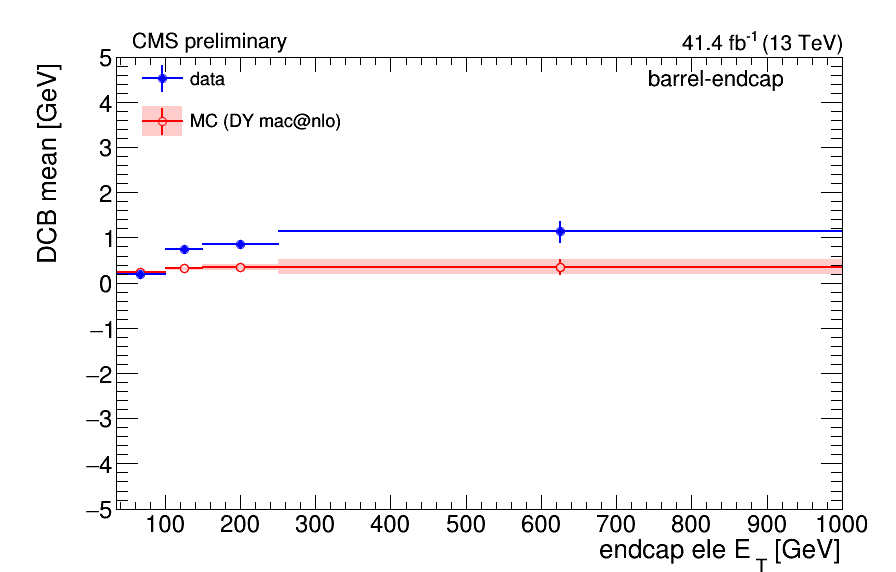
\includegraphics[width=0.48\textwidth]{figures/Zprime/2017/mass_resolution/scale_check/h_endcap_Et_Mee_BE_scale} &
      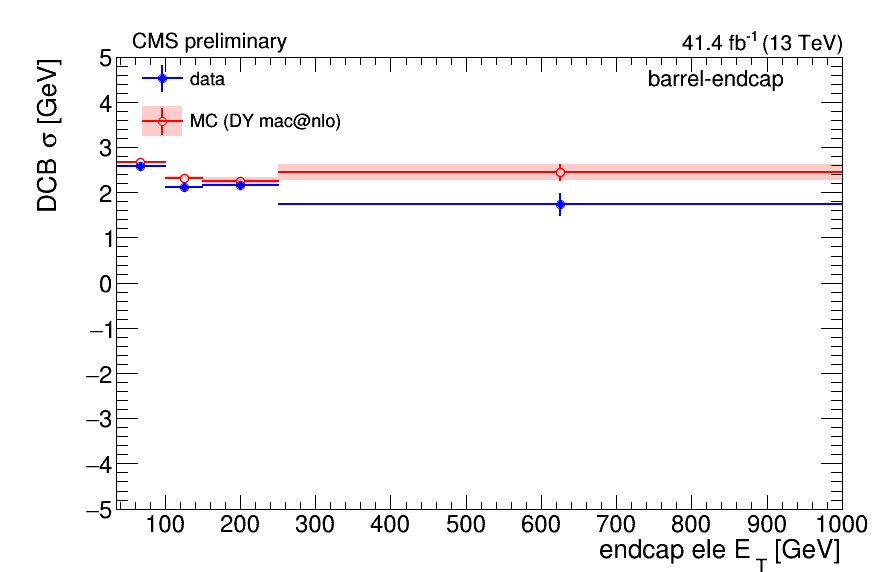
\includegraphics[width=0.48\textwidth]{figures/Zprime/2017/mass_resolution/scale_check/h_endcap_Et_Mee_BE_resolution} \\
      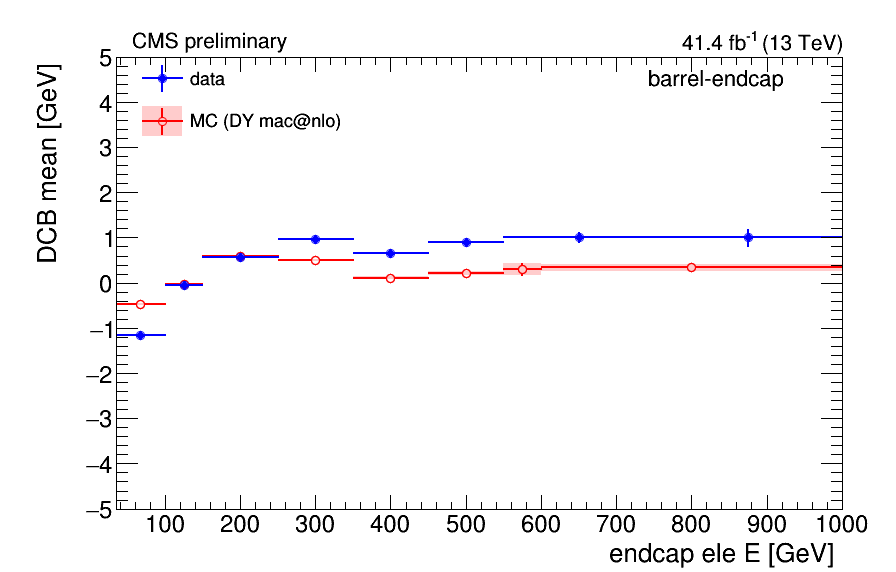
\includegraphics[width=0.48\textwidth]{figures/Zprime/2017/mass_resolution/scale_check/h_endcap_E_Mee_BE_scale} &
      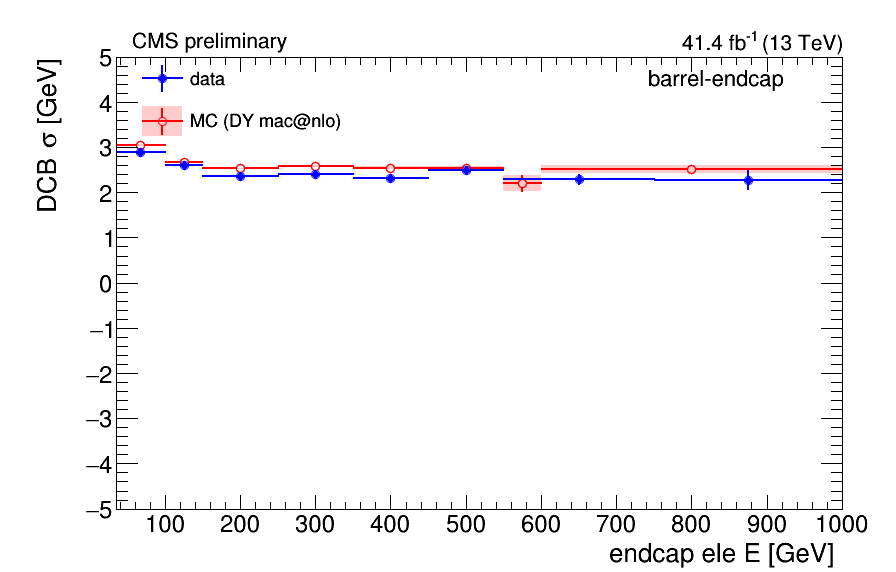
\includegraphics[width=0.48\textwidth]{figures/Zprime/2017/mass_resolution/scale_check/h_endcap_E_Mee_BE_resolution}
    \end{tabular}
    \caption{The mean (left) and sigma (right) values of dCB as the function of \et (top) and energy (bottom) of endcap electron for barrel-endcap channel.
    \label{fig:data_MC_Et_E_BE}}
  \end{center}
\end{figure}

\begin{figure}[ht]
  \begin{center}
    \begin{tabular}{cc}
      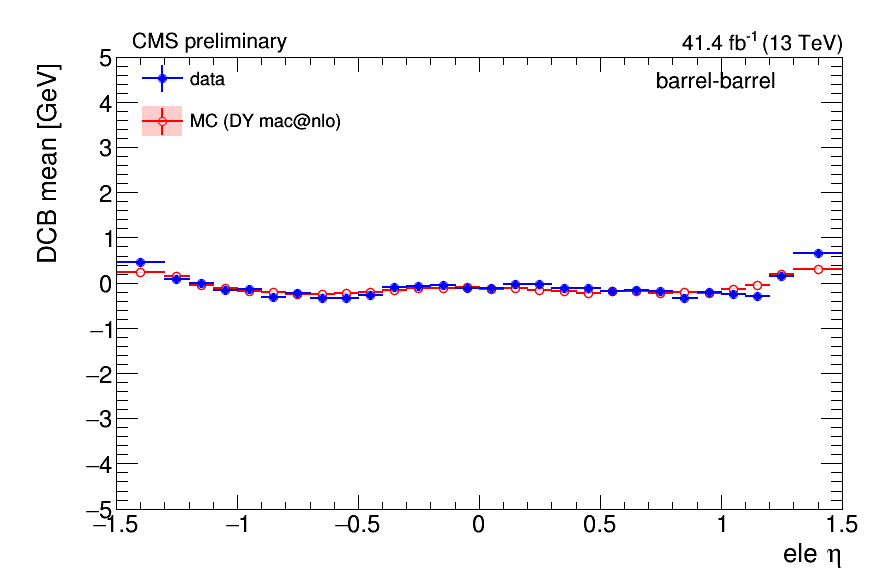
\includegraphics[width=0.48\textwidth]{figures/Zprime/2017/mass_resolution/scale_check/h_float_eta_Mee_BB_scale} &
      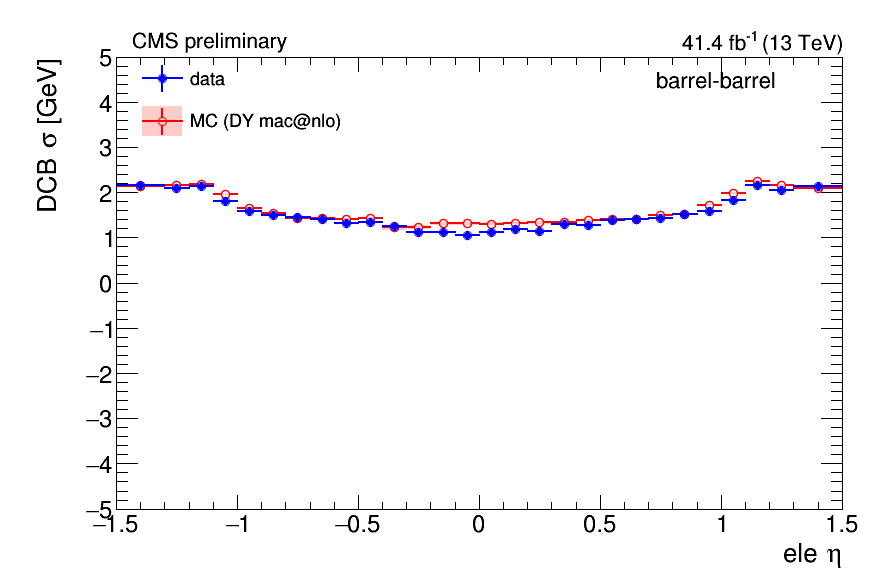
\includegraphics[width=0.48\textwidth]{figures/Zprime/2017/mass_resolution/scale_check/h_float_eta_Mee_BB_resolution} \\
      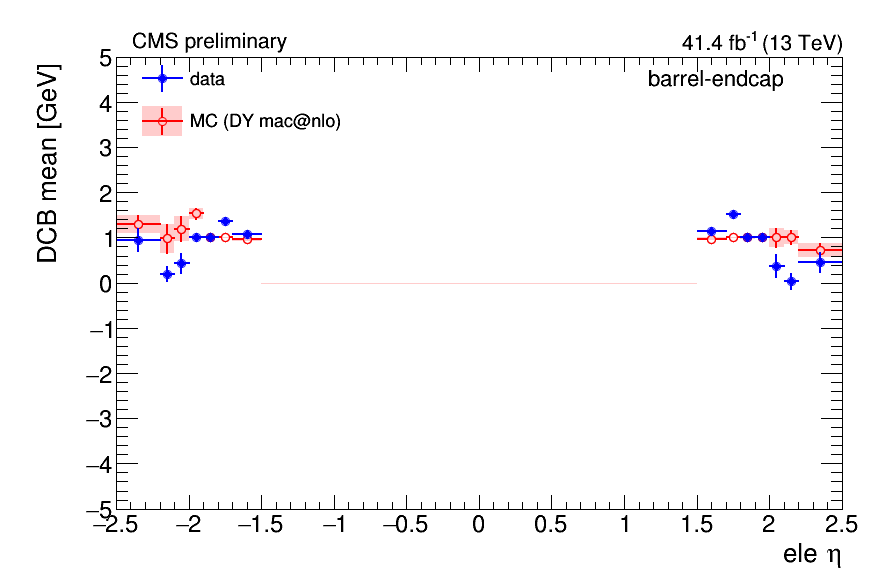
\includegraphics[width=0.48\textwidth]{figures/Zprime/2017/mass_resolution/scale_check/h_endcap_eta_Mee_BE_scale} &
      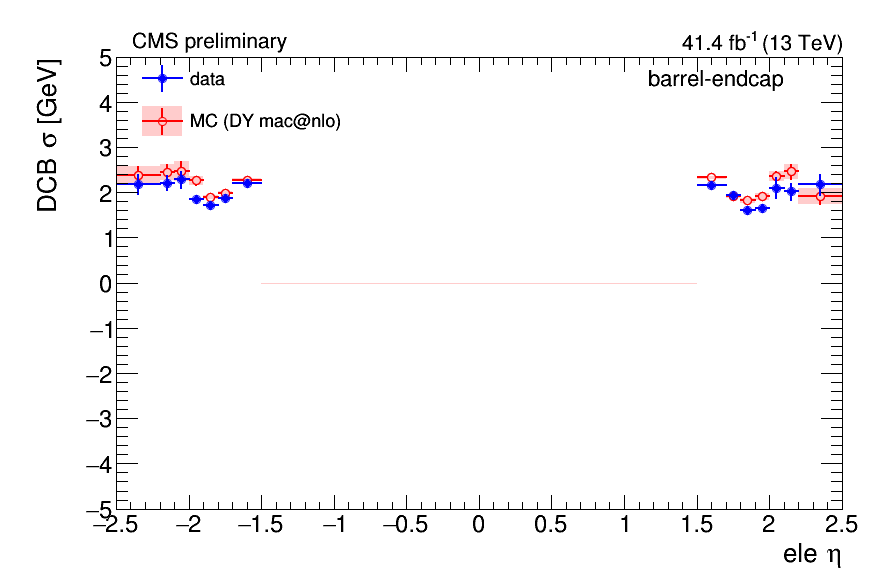
\includegraphics[width=0.48\textwidth]{figures/Zprime/2017/mass_resolution/scale_check/h_endcap_eta_Mee_BE_resolution}
    \end{tabular}
    \caption{The mean (left) and sigma (right) values of dCB as the function of $\eta$ of second electron (the first electron is asked to have $|\eta|<0.5$) for barrel-barrel (top) and barrel-endcap (bottom) channels.
    \label{fig:data_MC_eta_BB_BE}}
  \end{center}
\end{figure}





The second step of the study is based on MC only.
In particular, the mass resolution has been studied as a function of the generated invariant mass of the electron pair $m_{gen}$.
In order to maximise the statistics, different mass bin (from 200-5000 GeV) DY samples are used.

For each bin of the generated invariant mass $m_{gen}$, the distribution of the difference between the reconstructed and the generated invariant mass,
divided for the generated invariant mass is analyzed.
Defining a variable $resolution =\frac{m_{reco}-m_{gen}}{m_{gen}}$, its distribution is then acquired as a function of $m_{gen}$, and a maximum-likelihood
fit to the distribution in each mass bin is performed using a ``Cruijff function'' (which is defined as a Gaussian core connected with an exponential tail on each side) in 2016. While in 2017, the dCB function is used for the fit because it is found that the Cruijff is not able to correctly describe the invariant mass shape at very high mass due to electron saturation effects \footnote{When the deposite energy in single ECAL crystal is very high, the electric readout will be saturated because of limited dynamic range. See more details in Appendix \ref{app:Saturation}}.
Finally, the sigma parameter ($\sigma_{fit}$) of the fit function is added in quadrature with the $\sigma_{extra}$ coming from the first step of the study.

The fitted parameters are studied in their behaviour versus the corresponding generated mass and an analytic parametrisation is provided and used
as an input for the limit setting procedure (more details are given in appendix \ref{app:_mas_res}).
Results of mass resolution for the BB and BE regions are shown in Figure \ref{fig:resolution}.

\begin{figure}[ht]
\centering
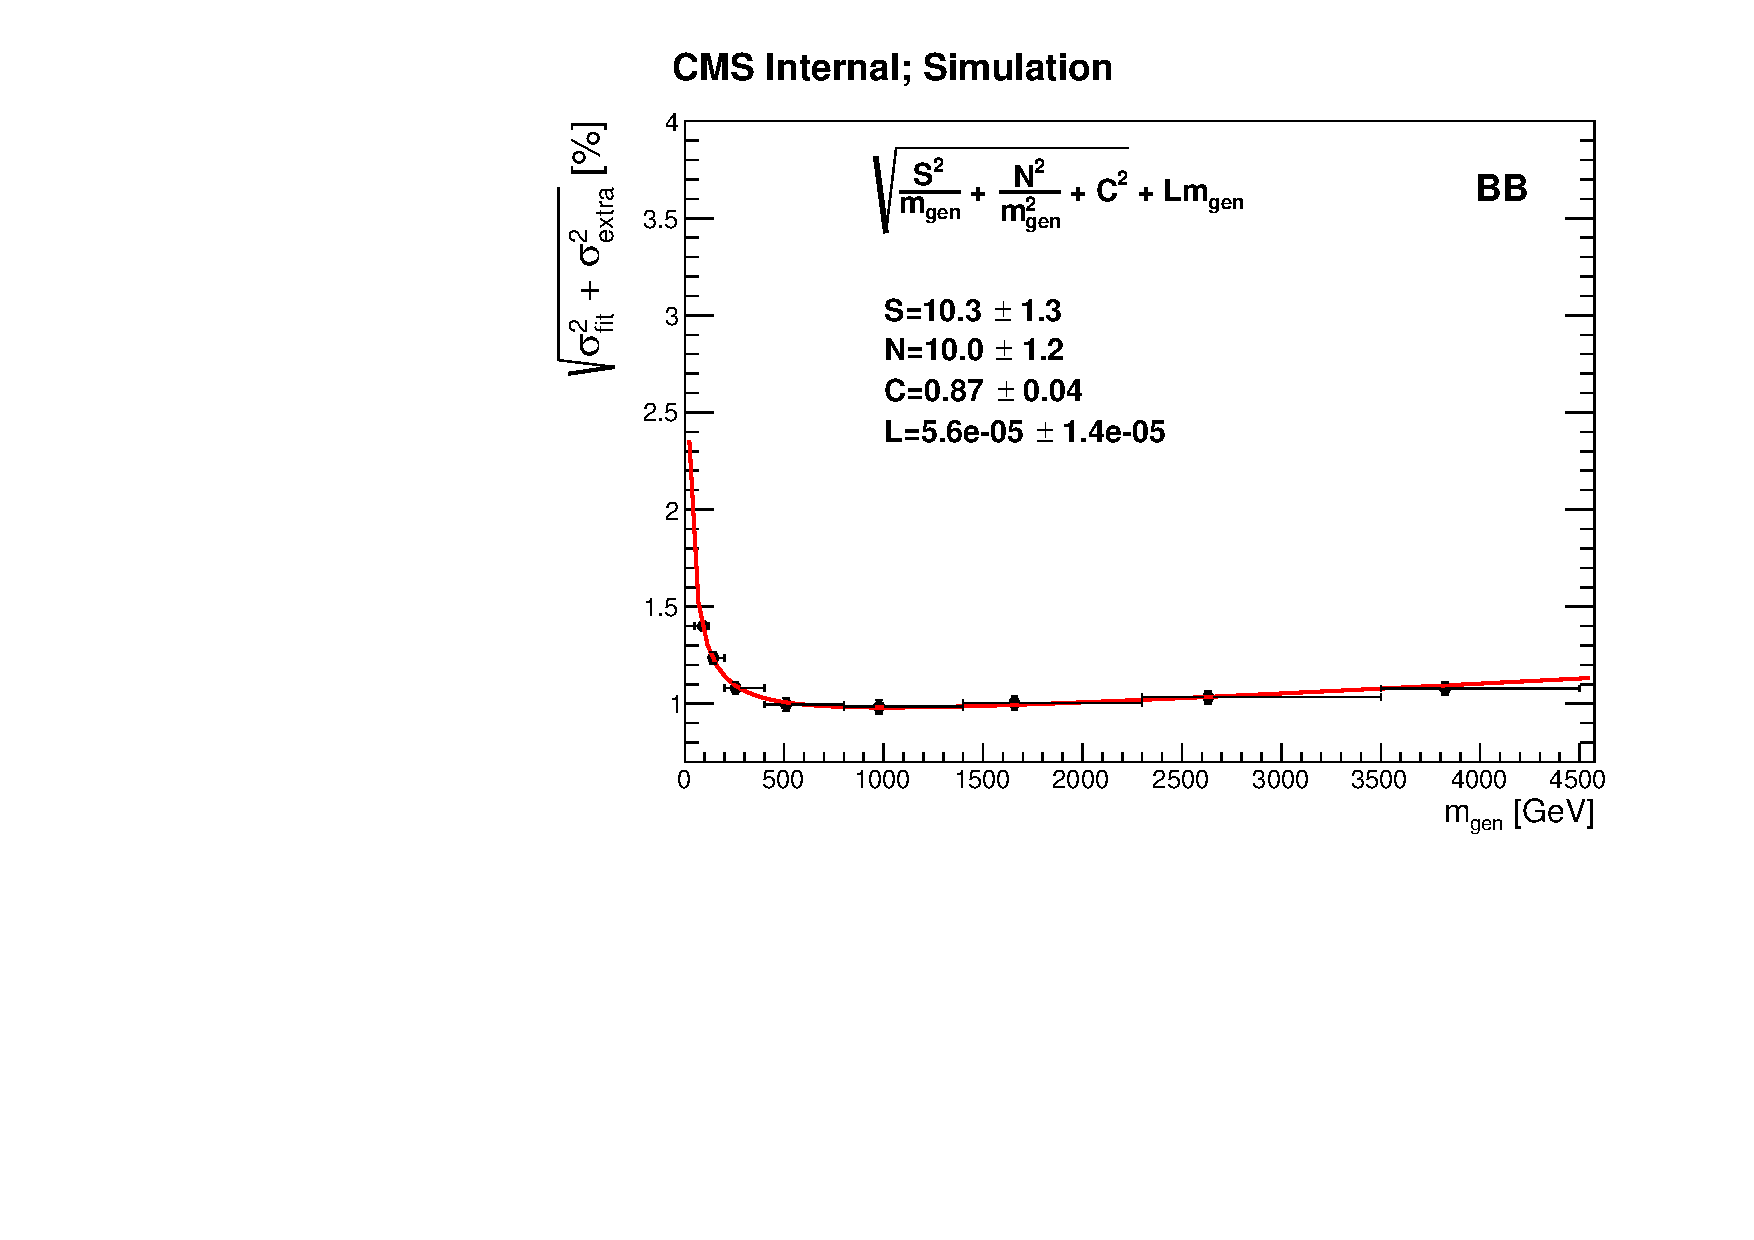
\includegraphics[width=0.48\textwidth]{figures/Zprime/2016/mass_resolution/resolution_BB.pdf}
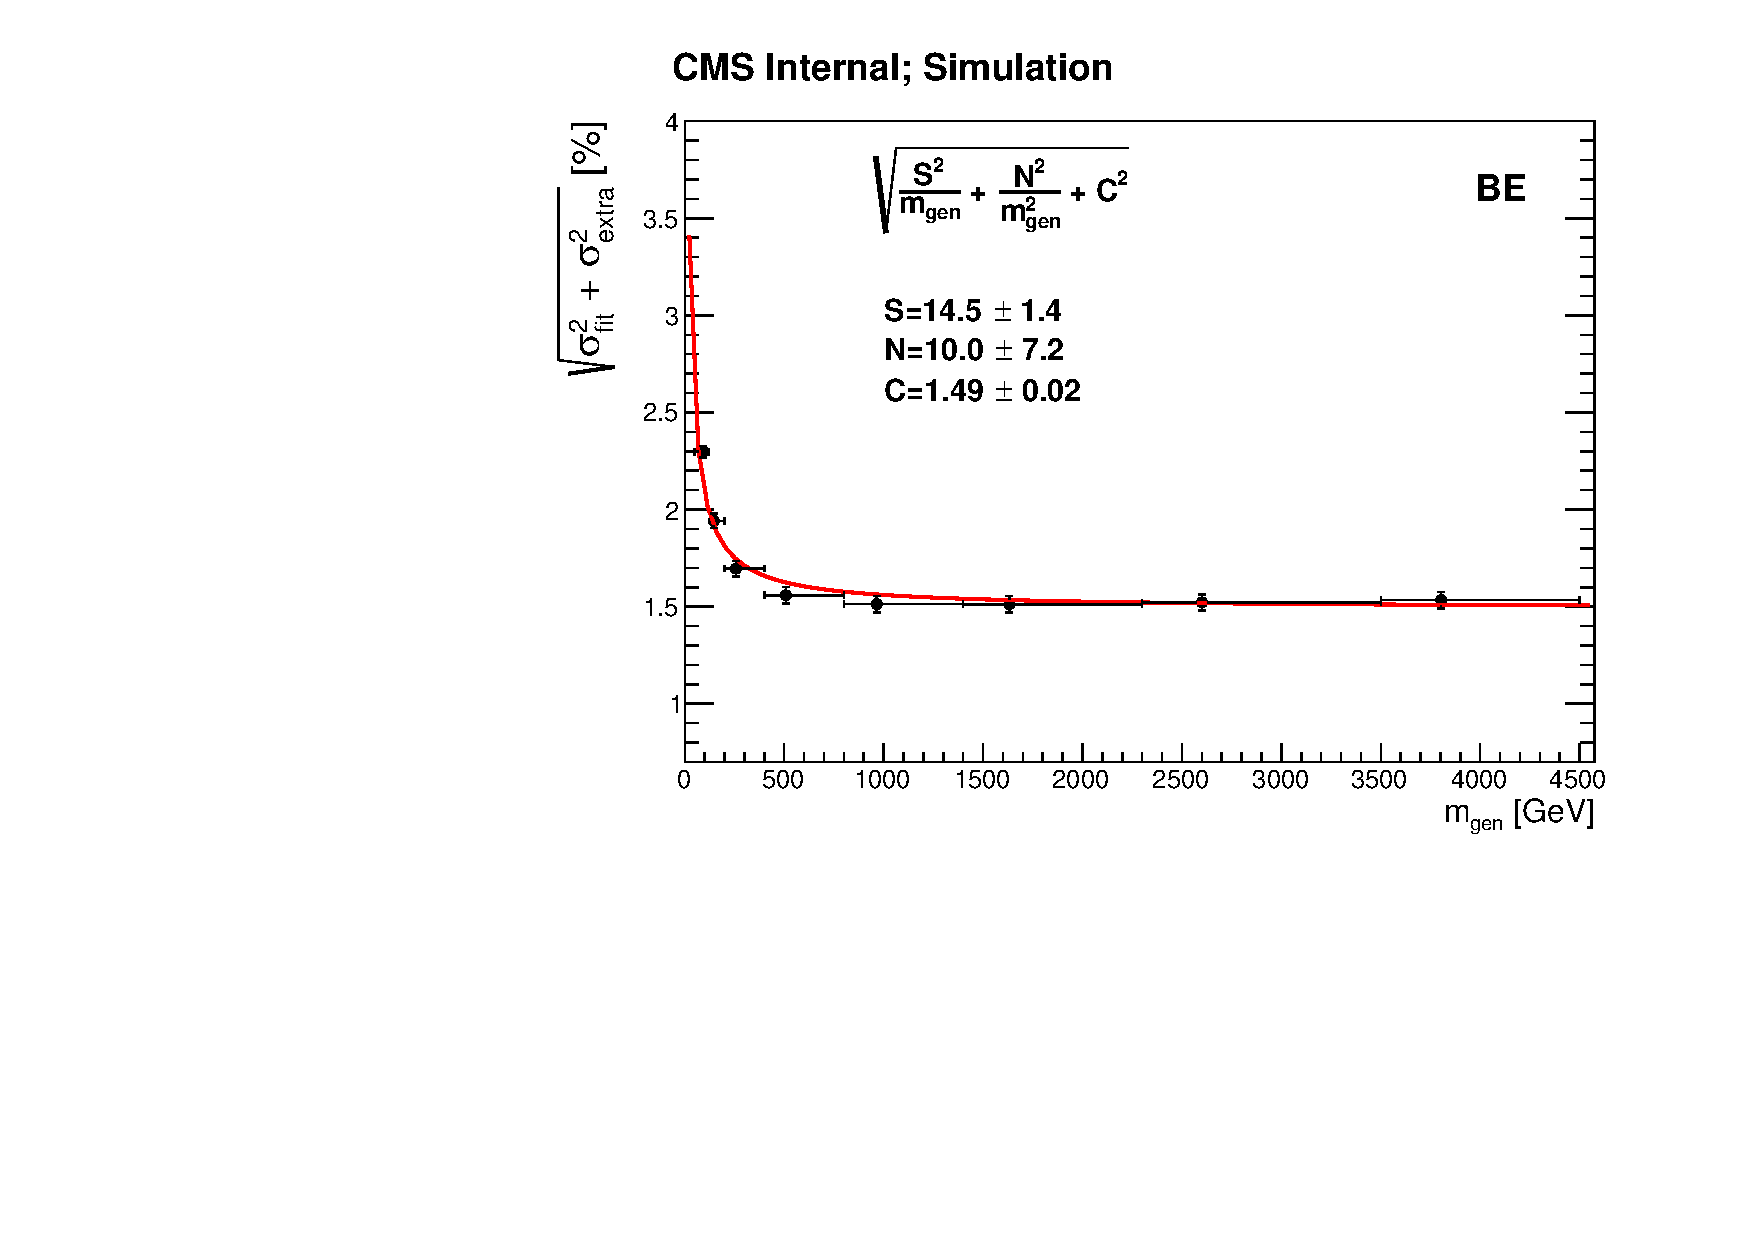
\includegraphics[width=0.48\textwidth]{figures/Zprime/2016/mass_resolution/resolution_BE.pdf}
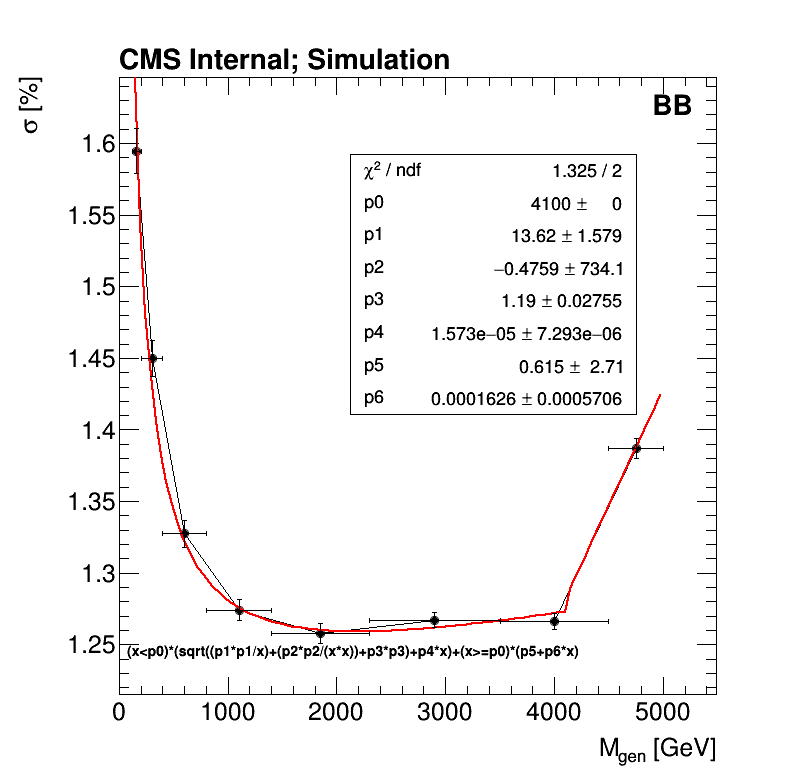
\includegraphics[width=0.48\textwidth]{figures/Zprime/2017/mass_resolution/High_Mass/BB_sigma}
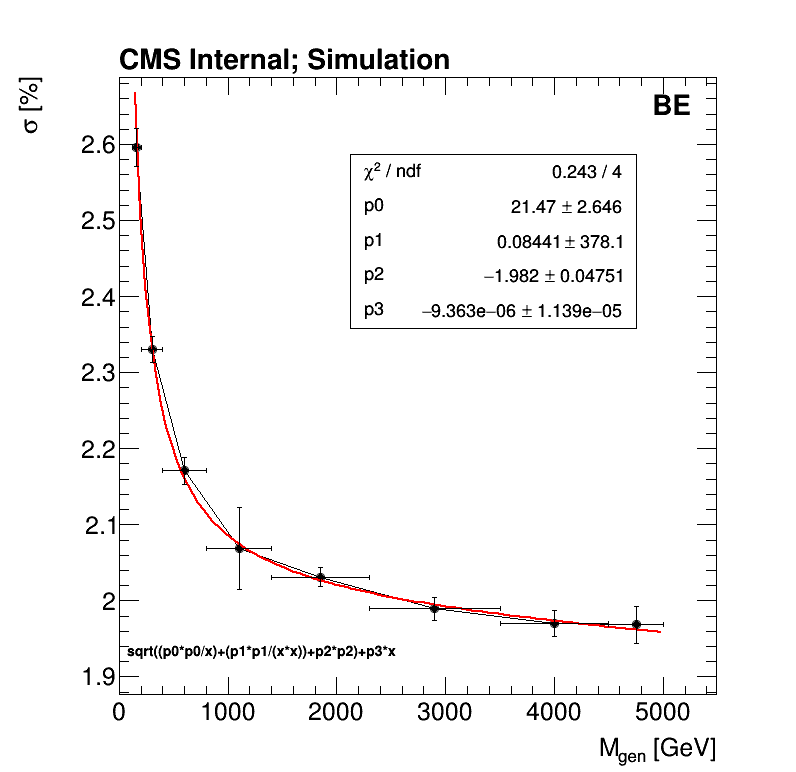
\includegraphics[width=0.48\textwidth]{figures/Zprime/2017/mass_resolution/High_Mass/BE_sigma}
\caption{The mass resolutions ($\sigma_{fit}$) as a function of generated Z boson mass for BB (left) and BE (right) regions in 2016 (top) \cite{CMS-AN-2016-404} and 2017 (bottom).
 \label{fig:resolution}}
\end{figure}

%The binning of the $x-$axis is chosen in order to have a reasonable amount of statistics for each range of $m_{ee}$ and ensure in this way a good quality, in terms
%of reduced $\chi^{2}$, of the performed fits.
%Some fit results are shown in Fig. \ref{fig:fits_BB} for the BB region, corresponding from left to right to the first bin of the mass resolution plot, the minimum of the mass resolution (encountered around $\approx$~1 TeV), and the last bin.
%\begin{figure}[ht]
%\centering
%\includegraphics[width=0.3\textwidth]{fig/mass_resolution/h_resolution_BB_1_bin_0.pdf}
%\includegraphics[width=0.3\textwidth]{fig/mass_resolution/h_resolution_BB_5_bin_4.pdf}
%\includegraphics[width=0.3\textwidth]{fig/mass_resolution/h_resolution_BB_19_bin_11.pdf}
%\caption{Fit results for the mass resolution, in the BB region.
% \label{fig:fits_BB}}
%\end{figure}

%With the same logic, some fit results are shown in Fig. \ref{fig:fits_BE} for the BE region, corresponding from left to right to the minimum of the mass resolution (encountered between 1-2 TeV), and the last two bins.
%
%\begin{figure}[ht]
%\centering
%\includegraphics[width=0.3\textwidth]{fig/mass_resolution/h_resolution_BE_7_bin_5.pdf}
%\includegraphics[width=0.3\textwidth]{fig/mass_resolution/h_resolution_BE_13_bin_7.pdf}
%\includegraphics[width=0.3\textwidth]{fig/mass_resolution/h_resolution_BE_17_bin_8.pdf}
%\caption{Fit results for the mass resolution, in the BE region.
% \label{fig:fits_BE}}
%\end{figure}

In the BB region there is a small linear rise in the mass resolution starting around $\approx$ 1.5 TeV. The effect has been already studied in \cite{CMS-AN-2015-222} and it is due to leakage of the electromagnetic ECAL shower in the HCAL subdetector which worsen in this way the energy reconstruction driven by the ECAL detector.
In fact, the effect of the leakage in the HCAL subdetector is visible as an increase in the $H/E$ variable, which is the ratio between the energy in the HCAL over the energy contained in the ECAL detector around the electron direction. For the increase of mass resolution from 4.5 TeV to 5 TeV in BB region is because the saturation effect becomes significant.
%The mean of $H_1/E_1 + H_2/E_2$ is shown in Figure \ref{fig:hoe}, where $1$ and $2$ label the first and the second electron, as a function of the invariant mass $m_{gen}$. Only in the BB region there is an increase at high mass, while in the BE region it stays rather flat.

%\begin{figure}[ht]
%\centering
%\includegraphics[width=0.48\textwidth]{fig/mass_resolution/HoverE_BB.pdf}
%\includegraphics[width=0.48\textwidth]{fig/mass_resolution/HoverE_BE.pdf}
%\caption{Mean of $H_1/E_1 + H_2/E_2$ as a function of the generated invariant mass for the BB region (left) and BE (right) channel.
% \label{fig:hoe}}
%\end{figure}

%It is also possible to quantify the leakage in the HCAL subdetector considering the behavior of $(H_1 + H_2)/(E_1 + E_2)$, where again $1$ and $2$ label the first and the second electron, as a function of the invariant mass $m_{gen}$. The behavior is very similar to the one of the other possible variable $H_1/E_1 + H_2/E_2$, apart from the absolute y-axis scale (See Figure \ref{fig:hoe_tot}).

%\begin{figure}[ht]
%\centering
%\includegraphics[width=0.48\textwidth]{fig/mass_resolution/HTotoverETot_BB.pdf}
%\includegraphics[width=0.48\textwidth]{fig/mass_resolution/HTotoverETot_BE.pdf}
%\caption{Mean of $(H_1 + H_2)/(E_1 + E_2)$ as a function of the generated invariant mass for the BB region (left) and BE (right) channel.
% \label{fig:hoe_tot}}
%\end{figure}

%As a cross-check in support of the HCAL leakage explanation, it is possible to show that the $\eta$ distribution for electrons in the ECAL barrel is different for the BB
%and BE category: in particular the electrons belonging to the BB category can be both low-$\eta$ and high-$\eta$ electrons, while in BE category there are mostly high-$\eta$
%electrons (see Figure \ref{fig:eta_check}.)

%\begin{figure}[!htbp]
%\begin{center}
%\includegraphics[width=0.48\textwidth]{fig/mass_resolution/eta_distributions.png}
%\end{center}
%\caption{$|\eta|$ distribution for the electrons falling in the ECAL barrel for BB category and BE category}
%\label{fig:eta_check}
%\end{figure}


%As a cross-check in support of the HCAL leakage explanation, the reconstructed energy is corrected, simply adding linearly the $H/E$ energetic fraction, without taking into account extra calibration coefficients. With this simple implementation, the resolution in the BB category appear much flatter at high $m_{gen}$ and in this configuration the rise is less pronounced, consisting in a 0.1 \% effect (See fig. \ref{fig:resolution_recover}).
%
%\begin{figure}[ht]
%\centering
%\includegraphics[width=0.6\textwidth]{fig/mass_resolution/resolution_h_recover_BB.pdf}
%\caption{Mass resolution as a function of the generated invariant mass for the BB category. The reconstructed energy is corrected to take into account the leakage in the HCAL subdetector.
% \label{fig:resolution_recover}}
%\end{figure}
%
%
%
%Finally, it is interesting to compare the obtained mass resolution plots with the ones that could be obtained using the raw-supercluster energy as reconstructed energy,
%so taking away the additional corrections applied in order to match the Z peak in data and MC.
%The comparison between those 2 possibilities (with the full reconstructed energy and using only the raw energy) are shown in Fig. \ref{fig:comparison_res}.
%
%\begin{figure}[ht]
%\centering
%\includegraphics[width=0.48\textwidth]{fig/mass_resolution/resolution_BB_comparison.png}
%\includegraphics[width=0.48\textwidth]{fig/mass_resolution/resolution_BE_comparison.png}
%\caption{Comparison between the mass resolution obtained using the full reconstructed energy (black points) and the raw-supercluster energy (red points) as a function of the generated invariant mass for the BB region (left) and BE (right) channel.
% \label{fig:comparison_res}}
%\end{figure}
%
%The comparison shows that in both regions, at high mass, the two different configurations tend to converge and, apart from some fluctations they show similar behavior.
\medskip
Also the mass scale of the ECAL detector has been studied as a function of the generated invariant mass of the electron pair $m_{gen}$, using the same generated samples taken into account for the mass resolution determination.

Defining the mass scale variable as $scale =\frac{m_{reco}}{m_{gen}}$, where $m_{gen}$ is the generated invariant mass, $m_{reco}$ is the reconstructed invariant mass. From the $resolution$ variable defined above it is easy to see that $scale= \frac{m_{reco}}{m_{gen}}= 1 + resolution$.
Therefore, the mass scale is taken from the mean parameter of the function used to fit the $resolution$ distribution and simply adding the unity to it. Besides, the error on the mean parameter is taken accordingly.

Results of mass scale for the BB and BE regions are shown in Figure \ref{fig:scale}.

\begin{figure}[ht]
\centering
\includegraphics[width=0.48\textwidth]{figures/Zprime/2016/mass_resolution/scale_BB.pdf}
\includegraphics[width=0.48\textwidth]{figures/Zprime/2016/mass_resolution/scale_BE.pdf}
\includegraphics[width=0.48\textwidth]{figures/Zprime/2017/mass_resolution/High_Mass/BB_mean}
\includegraphics[width=0.48\textwidth]{figures/Zprime/2017/mass_resolution/High_Mass/BE_mean}
\caption{The mass scales as a function of generated Z boson mass for BB (left) and BE (right) regions in 2016 (top) \cite{CMS-AN-2016-404} and 2017 (bottom).
 \label{fig:scale}}
\end{figure}

In the BB region there is a drop in the mass scale parameter starting around $\approx$ 1 TeV ($\approx$ 0.5 \% effect), which is the counterpart of the rise observed in the mass resolution, and is again due to leakage of a small part of the high-energetic electromagnetic shower in the HCAL subdetector.

\clearpage
\section{HEEP ID Efficiency and Scale Factor}\label{sec:Zprime_SF}
The MC samples used for the High Energy Electron Pair (HEEP) selection efficiency measurement and the scale factor measurement are listed in Table \ref{tab:HEEPSF-samples}.
\begin{table}[htp]
  \begin{center}
\small
\smallskip\noindent
\resizebox{\linewidth}{!}{%
\begin{tabular}{|l|l|l|}
\hline
Sample                                                                  & Xsection(pb) & Comments \\
\hline
\hline
DYToEE\_NNPDF30\_ 13TeV-powheg-pythia8                                 & 1921.8   & for 2016 $Z\rightarrow ee$     \\
\hline
DYJetsToLL\_M-50\_TuneCUETP8M1\_13TeV-madgraphMLM-pythia8              & 5765.4   & for 2016 $Z\rightarrow\tau\tau$        \\
DYJetsToLL\_M-50\_TuneCP5\_13TeV-amcatnloFXFX-pythia8                  & 5765.4   & for 2017 $Z\rightarrow ee$, $Z\rightarrow\tau\tau$        \\
\hline
WJetsToLNu\_TuneCUETP8M1\_13TeV-madgraphMLM-pythia8                    & 61526.7  & for 2016, 2017       \\
\hline
TT\_TuneCUETP8M2T4\_13TeV-powheg                                        & 831.76  & for 2016             \\
TTTo2L2Nu\_TuneCP5\_13TeV-powheg-pythia8                                & 87.31   & for 2017             \\
TTToSemiLeptonic\_TuneCP5\_PSweights\_13TeV-powheg-pythia8              & 366.6   & for 2017             \\
ST\_tW\_top\_5f\_inclusiveDecays\_13TeV-powheg-pythia8                  & 35.6    & for 2016, 2017       \\
ST\_tW\_antitop\_5f\_inclusiveDecays\_13TeV-powheg-pythia8              & 35.6    & for 2016, 2017        \\
\hline
GJets\_HT-40To100\_TuneCUETP8M1\_13TeV-madgraphMLM-pythia8              & 20790   & for 2016, 2017         \\
GJets\_HT-100To200\_TuneCUETP8M1\_13TeV-madgraphMLM-pythia8             & 9238    & for 2016, 2017         \\
GJets\_HT-200To400\_TuneCUETP8M1\_13TeV-madgraphMLM-pythia8             & 2305    & for 2016, 2017         \\
GJets\_HT-400To600\_TuneCUETP8M1\_13TeV-madgraphMLM-pythia8             & 274.4   & for 2016, 2017        \\
GJets\_HT-600ToInf\_TuneCUETP8M1\_13TeV-madgraphMLM-pythia8             & 93.46   & for 2016, 2017         \\
\hline
WW\_TuneCUETP8M1\_13TeV-pythia8                                         & 118.7   & for 2016, 2017         \\
WZ\_TuneCUETP8M1\_13TeV-pythia8                                         & 47.13   & for 2016, 2017         \\
ZZ\_TuneCUETP8M1\_13TeV-pythia8                                         & 16.523  & for 2016, 2017         \\
\hline
\end{tabular}}
\caption{MC samples used in the HEEP efficiency and scale factor studies}
\label{tab:HEEPSF-samples}
  \end{center}
\end{table}


\subsection{Tag and probe method}
\label{subsubsec:Same_sign_method}
A so called ``tag and probe'' method is often used for calculating a certain selection efficiency. For the HEEP ID efficiency study, this method starts by searching for a good electron (the ``tag'') which satisfies certain types of criteria. Then the efficiency of the interested selection cut is measured on the second electron candidate called the ``probe''.

The tag is required to fulfill the following conditions and is paired with every other gsf electron candidate in the event that passes the \et and $\eta$ acceptance cuts of the HEEP ID (probe).
\begin{itemize}
  \item[$\bullet$] tag must pass the HEEP ID
  \item[$\bullet$] tag must be a barrel electron
  \item[$\bullet$] tag must be matched to the \texttt{HLT\_Ele27\_eta2p1\_WPTight} (\texttt{HLT\_Ele35\_WPTight}) trigger in data in 2016 (2017)
\end{itemize}
The invariant mass of the tag and probe must satisfy $70 < \mathrm{M_{ee}} < 110 ~\mathrm{GeV}$. If there are multiple tag and probe candidates in an event then all pairs are selected.
When there are two tags in a pair, both are considered to be probes (e.g. once as ``$e_1 = tag , e_2 = probe$'' and once as ``$e_1 = probe , e_2 = tag$'') and by doing this we can get more statistics.
What we get is a very clear peak around the mass of the Z boson.
Therefore, we are confident that the electrons we have selected are almost real electrons coming from Z boson decay. Although there is a low contamination from other standard model backgrounds.

The efficiency is defined as
\begin{equation}
\label{SF:eq:eff}
\epsilon_{\text{HEEP}} = \frac{N_{\text{passing probes}}}{N_{\text{all probes}}}
\end{equation}
where $N_{\text{all probes}}$ is the total number of selected probes and $N_{\text{passing probes}}$ is the number of probes passing HEEP ID selection criteria. The efficiency can be measured in data and MC as a function of different variables like \et of probe, $\eta$ of probe, $\phi$ of probe, etc.

For measuring the HEEP ID efficiency in data, events are selected from SingleElectron dataset using \texttt{HLT\_Ele27\_eta2p1\_WPTight} (\texttt{HLT\_Ele35\_WPTight}) trigger in 2016 (2017).

For finding HEEP ID efficiency in MC, various MC samples are used which can be found in Table \ref{tab:HEEPSF-samples}. MC events are weighted using the trigger turn on curve of \texttt{HLT\_Ele27\_eta2p1\_WPTight} (\texttt{HLT\_Ele35\_WPTight}) path (see Figures~\ref{fig:Ele27_2016} and ~\ref{fig:Ele35_2017} of section~\ref{sec:Other_HLT_efficiency}) to emulate the trigger efficiency instead of matching tag with the \\
\texttt{HLT\_Ele27\_eta2p1\_WPTight} (\texttt{HLT\_Ele35\_WPTight}) trigger object.
MC events are weighted to correct for difference between data and MC pileup distributions according to the standard procedure.

The contribution of QCD background, where tag and probe are misidentified jets, is extracted from data using the ``same-sign'' method.
In same-sign method, we use the fact that the probability of assigning positive or negative charge to the misidentified jet should be equal (LHC is proton proton collider and positive charged jets should be produced a bit more but we are not sensitive to that amount in this study).
Therefore, the number of probe and variable distributions of probe are similar for opposite sign and same sign tag and probe pairs from QCD process. On the other hand, all other standard model processes have opposite sign electron pairs and do not contribute to same sign control region. The other SM backgrounds are considered using MC simulations.

Because the HEEP ID efficiency is different in barrel and endcaps regions, the probes are separated in barrel and endcaps.
In Figure \ref{fig:SS_nominal_mee_2016}, the invariant mass distributions of selected tag and probe pairs are shown for all tag and probe pairs (top), tag and probe pairs in which probe passes HEEP ID selection cuts ``pass-pass'' (middle) and tag and probe pairs in which probe fails passing  HEEP ID selection cuts ``pass-fail'' (bottom). Figures \ref{fig:SS_nominal_Et_2016} to \ref{fig:SS_nominal_PV_2016} present the \et, $\eta$, $\phi$ distributions of the probes and the number of primary vertex for the selected tag and probe pairs event in 2016.
The corresponding distributions for the 2017 data are presented in Figures \ref{fig:SS_nominal_mee_2017} to \ref{fig:SS_nominal_PV_2017}.

\begin{figure}[htp]
  \begin{center}
    \begin{tabular}{cc}
      \includegraphics[width=0.45\textwidth]{figures/Zprime/2016/ScaleFactor/SameSign/nominal/stack_mee_Barrel_probes_PUW.png} &
      \includegraphics[width=0.45\textwidth]{figures/Zprime/2016/ScaleFactor/SameSign/nominal/stack_mee_Endcap_probes_PUW.png} \\
      \includegraphics[width=0.45\textwidth]{figures/Zprime/2016/ScaleFactor/SameSign/nominal/stack_mee_Barrel_pass_PUW.png} &
      \includegraphics[width=0.45\textwidth]{figures/Zprime/2016/ScaleFactor/SameSign/nominal/stack_mee_Endcap_pass_PUW.png}\\
      \includegraphics[width=0.45\textwidth]{figures/Zprime/2016/ScaleFactor/SameSign/nominal/stack_mee_Barrel_fail_PUW.png} &
      \includegraphics[width=0.45\textwidth]{figures/Zprime/2016/ScaleFactor/SameSign/nominal/stack_mee_Endcap_fail_PUW.png}
    \end{tabular}
    \caption{Invariant mass distributions of tag and probe for probe in the barrel (left) and endcap (right) where all the probes are included (top), only passing probes are included (middle), and only failed probes are included (bottom) for 2016.}
    \label{fig:SS_nominal_mee_2016}
  \end{center}
\end{figure}
\begin{figure}[htp]
  \begin{center}
    \begin{tabular}{cc}
      \includegraphics[width=0.45\textwidth]{figures/Zprime/2016/ScaleFactor/SameSign/nominal/stack_Et_Barrel_probes_PUW.png} &
      \includegraphics[width=0.45\textwidth]{figures/Zprime/2016/ScaleFactor/SameSign/nominal/stack_Et_Endcap_probes_PUW.png} \\
      \includegraphics[width=0.45\textwidth]{figures/Zprime/2016/ScaleFactor/SameSign/nominal/stack_Et_Barrel_pass_PUW.png} &
      \includegraphics[width=0.45\textwidth]{figures/Zprime/2016/ScaleFactor/SameSign/nominal/stack_Et_Endcap_pass_PUW.png}\\
      \includegraphics[width=0.45\textwidth]{figures/Zprime/2016/ScaleFactor/SameSign/nominal/stack_Et_Barrel_fail_PUW.png} &
      \includegraphics[width=0.45\textwidth]{figures/Zprime/2016/ScaleFactor/SameSign/nominal/stack_Et_Endcap_fail_PUW.png}
    \end{tabular}
    \caption{\et of probe in the barrel (left) and endcap (right) where all the probes are included (top), only passing probes are included (middle), and only failed probes are included (bottom) for 2016.}
    \label{fig:SS_nominal_Et_2016}
  \end{center}
\end{figure}
\begin{figure}[htp]
  \begin{center}
    \begin{tabular}{cc}
      \includegraphics[width=0.45\textwidth]{figures/Zprime/2016/ScaleFactor/SameSign/nominal/stack_eta_BE_Barrel+Endcap_probes_PUW.png} &
      \includegraphics[width=0.45\textwidth]{figures/Zprime/2016/ScaleFactor/SameSign/nominal/stack_eta_BE_Barrel+Endcap_pass_PUW.png} \\
      \includegraphics[width=0.45\textwidth]{figures/Zprime/2016/ScaleFactor/SameSign/nominal/stack_eta_BE_Barrel+Endcap_fail_PUW.png} &
    \end{tabular}
    \caption{$\eta$ of probe where all the probes are included (top left), only passing probes are included (top right), and only failed probes are included (bottom) for 2016.}
    \label{fig:SS_nominal_eta_2016}
  \end{center}
\end{figure}
\begin{figure}[htp]
  \begin{center}
    \begin{tabular}{cc}
      \includegraphics[width=0.45\textwidth]{figures/Zprime/2016/ScaleFactor/SameSign/nominal/stack_phi_Barrel_probes_PUW.png} &
      \includegraphics[width=0.45\textwidth]{figures/Zprime/2016/ScaleFactor/SameSign/nominal/stack_phi_Endcap_probes_PUW.png} \\
      \includegraphics[width=0.45\textwidth]{figures/Zprime/2016/ScaleFactor/SameSign/nominal/stack_phi_Barrel_pass_PUW.png} &
      \includegraphics[width=0.45\textwidth]{figures/Zprime/2016/ScaleFactor/SameSign/nominal/stack_phi_Endcap_pass_PUW.png}\\
      \includegraphics[width=0.45\textwidth]{figures/Zprime/2016/ScaleFactor/SameSign/nominal/stack_phi_Barrel_fail_PUW.png} &
      \includegraphics[width=0.45\textwidth]{figures/Zprime/2016/ScaleFactor/SameSign/nominal/stack_phi_Endcap_fail_PUW.png}
    \end{tabular}
    \caption{$\phi$ of probe in the barrel (left) and endcap (right) where all the probes are included (top), only passing probes are included (middle), and only failed probes are included (bottom) for 2016.}
    \label{fig:SS_nominal_phi_2016}
  \end{center}
\end{figure}
\begin{figure}[htp]
  \begin{center}
    \begin{tabular}{cc}
      \includegraphics[width=0.45\textwidth]{figures/Zprime/2016/ScaleFactor/SameSign/nominal/stack_nVtx_Barrel_probes_PUW.png} &
      \includegraphics[width=0.45\textwidth]{figures/Zprime/2016/ScaleFactor/SameSign/nominal/stack_nVtx_Endcap_probes_PUW.png} \\
      \includegraphics[width=0.45\textwidth]{figures/Zprime/2016/ScaleFactor/SameSign/nominal/stack_nVtx_Barrel_pass_PUW.png} &
      \includegraphics[width=0.45\textwidth]{figures/Zprime/2016/ScaleFactor/SameSign/nominal/stack_nVtx_Endcap_pass_PUW.png}\\
      \includegraphics[width=0.45\textwidth]{figures/Zprime/2016/ScaleFactor/SameSign/nominal/stack_nVtx_Barrel_fail_PUW.png} &
      \includegraphics[width=0.45\textwidth]{figures/Zprime/2016/ScaleFactor/SameSign/nominal/stack_nVtx_Endcap_fail_PUW.png}
    \end{tabular}
    \caption{Number of primary vertex of tag and probe pair event in the barrel (left) and endcap (right) where all the probes are included (top), only passing probes are included (middle), and only failed probes are included (bottom) for 2016.}
    \label{fig:SS_nominal_PV_2016}
  \end{center}
\end{figure}



\begin{figure}[htp]
  \begin{center}
    \begin{tabular}{cc}
      \includegraphics[width=0.45\textwidth]{figures/Zprime/2017/ScaleFactor/SameSign/nominal/stack_mee_Barrel_probes_PUW.png} &
      \includegraphics[width=0.45\textwidth]{figures/Zprime/2017/ScaleFactor/SameSign/nominal/stack_mee_Endcap_probes_PUW.png} \\
      \includegraphics[width=0.45\textwidth]{figures/Zprime/2017/ScaleFactor/SameSign/nominal/stack_mee_Barrel_pass_PUW.png} &
      \includegraphics[width=0.45\textwidth]{figures/Zprime/2017/ScaleFactor/SameSign/nominal/stack_mee_Endcap_pass_PUW.png}\\
      \includegraphics[width=0.45\textwidth]{figures/Zprime/2017/ScaleFactor/SameSign/nominal/stack_mee_Barrel_fail_PUW.png} &
      \includegraphics[width=0.45\textwidth]{figures/Zprime/2017/ScaleFactor/SameSign/nominal/stack_mee_Endcap_fail_PUW.png}
    \end{tabular}
    \caption{Invariant mass of tag and probe distributions for probe in the barrel (left) and endcap (right) where all the probes are included (top), only passing probes are included (middle), and only failed probes are included (bottom) for 2017.}
    \label{fig:SS_nominal_mee_2017}
  \end{center}
\end{figure}
\begin{figure}[htp]
  \begin{center}
    \begin{tabular}{cc}
      \includegraphics[width=0.45\textwidth]{figures/Zprime/2017/ScaleFactor/SameSign/nominal/stack_Et_Barrel_probes_PUW.png} &
      \includegraphics[width=0.45\textwidth]{figures/Zprime/2017/ScaleFactor/SameSign/nominal/stack_Et_Endcap_probes_PUW.png} \\
      \includegraphics[width=0.45\textwidth]{figures/Zprime/2017/ScaleFactor/SameSign/nominal/stack_Et_Barrel_pass_PUW.png} &
      \includegraphics[width=0.45\textwidth]{figures/Zprime/2017/ScaleFactor/SameSign/nominal/stack_Et_Endcap_pass_PUW.png}\\
      \includegraphics[width=0.45\textwidth]{figures/Zprime/2017/ScaleFactor/SameSign/nominal/stack_Et_Barrel_fail_PUW.png} &
      \includegraphics[width=0.45\textwidth]{figures/Zprime/2017/ScaleFactor/SameSign/nominal/stack_Et_Endcap_fail_PUW.png}
    \end{tabular}
    \caption{\et of probe in the barrel (left) and endcap (right) where all the probes are included (top), only passing probes are included (middle), and only failed probes are included (bottom) for 2017.}
    \label{fig:SS_nominal_Et_2017}
  \end{center}
\end{figure}
\begin{figure}[htp]
  \begin{center}
    \begin{tabular}{cc}
      \includegraphics[width=0.45\textwidth]{figures/Zprime/2017/ScaleFactor/SameSign/nominal/stack_eta_BE_Barrel+Endcap_probes_PUW.png} &
      \includegraphics[width=0.45\textwidth]{figures/Zprime/2017/ScaleFactor/SameSign/nominal/stack_eta_BE_Barrel+Endcap_pass_PUW.png} \\
      \includegraphics[width=0.45\textwidth]{figures/Zprime/2017/ScaleFactor/SameSign/nominal/stack_eta_BE_Barrel+Endcap_fail_PUW.png} &
    \end{tabular}
    \caption{$\eta$ of probe where all the probes are included (top left), only passing probes are included (top right), and only failed probes are included (bottom) for 2017.}
    \label{fig:SS_nominal_eta_2017}
  \end{center}
\end{figure}
\begin{figure}[htp]
  \begin{center}
    \begin{tabular}{cc}
      \includegraphics[width=0.45\textwidth]{figures/Zprime/2017/ScaleFactor/SameSign/nominal/stack_phi_Barrel_probes_PUW.png} &
      \includegraphics[width=0.45\textwidth]{figures/Zprime/2017/ScaleFactor/SameSign/nominal/stack_phi_Endcap_probes_PUW.png} \\
      \includegraphics[width=0.45\textwidth]{figures/Zprime/2017/ScaleFactor/SameSign/nominal/stack_phi_Barrel_pass_PUW.png} &
      \includegraphics[width=0.45\textwidth]{figures/Zprime/2017/ScaleFactor/SameSign/nominal/stack_phi_Endcap_pass_PUW.png}\\
      \includegraphics[width=0.45\textwidth]{figures/Zprime/2017/ScaleFactor/SameSign/nominal/stack_phi_Barrel_fail_PUW.png} &
      \includegraphics[width=0.45\textwidth]{figures/Zprime/2017/ScaleFactor/SameSign/nominal/stack_phi_Endcap_fail_PUW.png}
    \end{tabular}
    \caption{$\phi$ of probe in the barrel (left) and endcap (right) where all the probes are included (top), only passing probes are included (middle), and only failed probes are included (bottom) for 2017.}
    \label{fig:SS_nominal_phi_2017}
  \end{center}
\end{figure}
\begin{figure}[htp]
  \begin{center}
    \begin{tabular}{cc}
      \includegraphics[width=0.45\textwidth]{figures/Zprime/2017/ScaleFactor/SameSign/nominal/stack_nVtx_Barrel_probes_PUW.png} &
      \includegraphics[width=0.45\textwidth]{figures/Zprime/2017/ScaleFactor/SameSign/nominal/stack_nVtx_Endcap_probes_PUW.png} \\
      \includegraphics[width=0.45\textwidth]{figures/Zprime/2017/ScaleFactor/SameSign/nominal/stack_nVtx_Barrel_pass_PUW.png} &
      \includegraphics[width=0.45\textwidth]{figures/Zprime/2017/ScaleFactor/SameSign/nominal/stack_nVtx_Endcap_pass_PUW.png}\\
      \includegraphics[width=0.45\textwidth]{figures/Zprime/2017/ScaleFactor/SameSign/nominal/stack_nVtx_Barrel_fail_PUW.png} &
      \includegraphics[width=0.45\textwidth]{figures/Zprime/2017/ScaleFactor/SameSign/nominal/stack_nVtx_Endcap_fail_PUW.png}
    \end{tabular}
    \caption{Number of primary vertex of tag and probe pair event in the barrel (left) and endcap (right) where all the probes are included (top), only passing probes are included (middle), and only failed probes are included (bottom) for 2017.}
    \label{fig:SS_nominal_PV_2017}
  \end{center}
\end{figure}

\clearpage
\subsection{HEEP ID efficiencies and scale factors}
\label{subsubsec:SF_results}
In 2016, the HEEP ID efficiencies for data and MC are shown as a functions of \et of the probe, $\eta$ of the probe, $\phi$ of the probe, and $N_{vtx}$ in Figures \ref{fig:eff_SS_nominal_ET_2016}-\ref{fig:eff_SS_nominal_nVtx_2016} (left), here data includes both DY and non-DY events. In order to check if the contributions of non-DY backgrounds are estimated correctly, the DY efficiency is compared to data from which non-DY contributions are subtracted in Figures \ref{fig:eff_SS_nominal_ET_2016}-\ref{fig:eff_SS_nominal_nVtx_2016} (right). The scale factors obtained with these two approaches are in a good agreement in all variables. In addition, the HEEP ID efficiency scale factors between data and MC are shown in the bottom pad of the same plot.
Same plots in 2017 are shown in Figures \ref{fig:eff_SS_nominal_ET_2017}-\ref{fig:eff_SS_nominal_nVtx_2017}.
\begin{figure}[htp]
  \begin{center}
    \begin{tabular}{cc}
      \includegraphics[width=0.45\textwidth]{figures/Zprime/2016/ScaleFactor/SameSign/nominal/g_compare_cut_Et_Barrel_ea_ta_inc_AS_nominal_PUW.png} &
      \includegraphics[width=0.45\textwidth]{figures/Zprime/2016/ScaleFactor/SameSign/nominal/g_compare_cut_Et_Barrel_ea_ta_exc_AS_nominal_PUW.png} \\
      \includegraphics[width=0.45\textwidth]{figures/Zprime/2016/ScaleFactor/SameSign/nominal/g_compare_cut_Et_Endcap_ea_ta_inc_AS_nominal_PUW.png} &
      \includegraphics[width=0.45\textwidth]{figures/Zprime/2016/ScaleFactor/SameSign/nominal/g_compare_cut_Et_Endcap_ea_ta_exc_AS_nominal_PUW.png}
    \end{tabular}
    \caption{The HEEP efficiencies in data and MC, as well as the scale factors when the probe is in the barrel (top) and endcap (bottom) where the non-DY processes are included (left) and subtracted (right) as functions of probe \et in 2016.}
    \label{fig:eff_SS_nominal_ET_2016}
  \end{center}
\end{figure}

\begin{figure}[htp]
  \begin{center}
    \begin{tabular}{cc}
      \includegraphics[width=0.45\textwidth]{figures/Zprime/2016/ScaleFactor/SameSign/nominal/g_compare_cut_eta_Barrel+Endcap_ea_ta_inc_AS_nominal_PUW.png} &
      \includegraphics[width=0.45\textwidth]{figures/Zprime/2016/ScaleFactor/SameSign/nominal/g_compare_cut_eta_Barrel+Endcap_ea_ta_exc_AS_nominal_PUW.png} \\
    \end{tabular}
    \caption{The HEEP efficiencies in data and MC, as well as the scale factors where the non-DY processes are included (left) and subtracted (right) as functions of probe $\eta$ in 2016.}
    \label{fig:eff_SS_nominal_eta_2016}
  \end{center}
\end{figure}

\begin{figure}[htp]
  \begin{center}
    \begin{tabular}{cc}
      \includegraphics[width=0.45\textwidth,height=6.3cm]{figures/Zprime/2016/ScaleFactor/SameSign/nominal/g_compare_cut_phi_Barrel_ea_ta_inc_AS_nominal_PUW.png} &
      \includegraphics[width=0.45\textwidth,height=6.3cm]{figures/Zprime/2016/ScaleFactor/SameSign/nominal/g_compare_cut_phi_Barrel_ea_ta_exc_AS_nominal_PUW.png} \\
      \includegraphics[width=0.45\textwidth,height=6.3cm]{figures/Zprime/2016/ScaleFactor/SameSign/nominal/g_compare_cut_phi_Endcap_ea_ta_inc_AS_nominal_PUW.png} &
      \includegraphics[width=0.45\textwidth,height=6.3cm]{figures/Zprime/2016/ScaleFactor/SameSign/nominal/g_compare_cut_phi_Endcap_ea_ta_exc_AS_nominal_PUW.png}
    \end{tabular}
    \caption{The HEEP efficiencies in data and MC, as well as the scale factors when the probe is in the barrel (top) and endcap (bottom) where the non-DY processes are included (left) and subtracted (right) as functions of probe $\phi$ in 2016.}
    \label{fig:eff_SS_nominal_phi_2016}
  \end{center}
\end{figure}

\begin{figure}[bh]
  \begin{center}
    \begin{tabular}{cc}
      \includegraphics[width=0.45\textwidth]{figures/Zprime/2016/ScaleFactor/SameSign/nominal/g_compare_cut_nVtx_Barrel_ea_ta_inc_AS_nominal_PUW.png} &
      \includegraphics[width=0.45\textwidth]{figures/Zprime/2016/ScaleFactor/SameSign/nominal/g_compare_cut_nVtx_Barrel_ea_ta_exc_AS_nominal_PUW.png} \\
      \includegraphics[width=0.45\textwidth]{figures/Zprime/2016/ScaleFactor/SameSign/nominal/g_compare_cut_nVtx_Endcap_ea_ta_inc_AS_nominal_PUW.png} &
      \includegraphics[width=0.45\textwidth]{figures/Zprime/2016/ScaleFactor/SameSign/nominal/g_compare_cut_nVtx_Endcap_ea_ta_exc_AS_nominal_PUW.png}
    \end{tabular}
    \caption{The HEEP efficiencies in data and MC, as well as the scale factors when the probe is in the barrel (top) and endcap (bottom) where the non-DY processes are included (left) and subtracted (right) as functions of the number of primary vertices, $n_{Vtx}$ in 2016.}
    \label{fig:eff_SS_nominal_nVtx_2016}
  \end{center}
\end{figure}


\begin{figure}[htp]
  \begin{center}
    \begin{tabular}{cc}
      \includegraphics[width=0.45\textwidth]{figures/Zprime/2017/ScaleFactor/SameSign/nominal/g_compare_cut_Et_Barrel_ea_ta_inc_AS_nominal_PUW.png} &
      \includegraphics[width=0.45\textwidth]{figures/Zprime/2017/ScaleFactor/SameSign/nominal/g_compare_cut_Et_Barrel_ea_ta_exc_AS_nominal_PUW.png} \\
      \includegraphics[width=0.45\textwidth]{figures/Zprime/2017/ScaleFactor/SameSign/nominal/g_compare_cut_Et_Endcap_ea_ta_inc_AS_nominal_PUW.png} &
      \includegraphics[width=0.45\textwidth]{figures/Zprime/2017/ScaleFactor/SameSign/nominal/g_compare_cut_Et_Endcap_ea_ta_exc_AS_nominal_PUW.png}
    \end{tabular}
    \caption{The HEEP efficiencies in data and MC, as well as the scale factors when the probe is in the barrel (top) and endcap (bottom) where the non-DY processes are included (left) and subtracted (right) as functions of probe \et in 2017.}
    \label{fig:eff_SS_nominal_ET_2017}
  \end{center}
\end{figure}

\begin{figure}[htp]
  \begin{center}
    \begin{tabular}{cc}
      \includegraphics[width=0.45\textwidth]{figures/Zprime/2017/ScaleFactor/SameSign/nominal/g_compare_cut_eta_Barrel+Endcap_ea_ta_inc_AS_nominal_PUW.png} &
      \includegraphics[width=0.45\textwidth]{figures/Zprime/2017/ScaleFactor/SameSign/nominal/g_compare_cut_eta_Barrel+Endcap_ea_ta_exc_AS_nominal_PUW.png} \\
    \end{tabular}
    \caption{The HEEP efficiencies in data and MC, as well as the scale factors where the non-DY processes are included (left) and subtracted (right) as functions of probe $\eta$ in 2017.}
    \label{fig:eff_SS_nominal_eta_2017}
  \end{center}
\end{figure}

\begin{figure}[htp]
  \begin{center}
    \begin{tabular}{cc}
      \includegraphics[width=0.45\textwidth,height=6.3cm]{figures/Zprime/2017/ScaleFactor/SameSign/nominal/g_compare_cut_phi_Barrel_ea_ta_inc_AS_nominal_PUW.png} &
      \includegraphics[width=0.45\textwidth,height=6.3cm]{figures/Zprime/2017/ScaleFactor/SameSign/nominal/g_compare_cut_phi_Barrel_ea_ta_exc_AS_nominal_PUW.png} \\
      \includegraphics[width=0.45\textwidth,height=6.3cm]{figures/Zprime/2017/ScaleFactor/SameSign/nominal/g_compare_cut_phi_Endcap_ea_ta_inc_AS_nominal_PUW.png} &
      \includegraphics[width=0.45\textwidth,height=6.3cm]{figures/Zprime/2017/ScaleFactor/SameSign/nominal/g_compare_cut_phi_Endcap_ea_ta_exc_AS_nominal_PUW.png}
    \end{tabular}
    \caption{The HEEP efficiencies in data and MC, as well as the scale factors when the probe is in the barrel (top) and endcap (bottom) where the non-DY processes are included (left) and subtracted (right) as functions of probe $\phi$ in 2017.}
    \label{fig:eff_SS_nominal_phi_2017}
  \end{center}
\end{figure}

\begin{figure}[bh]
  \begin{center}
    \begin{tabular}{cc}
      \includegraphics[width=0.45\textwidth]{figures/Zprime/2017/ScaleFactor/SameSign/nominal/g_compare_cut_nVtx_Barrel_ea_ta_inc_AS_nominal_PUW.png} &
      \includegraphics[width=0.45\textwidth]{figures/Zprime/2017/ScaleFactor/SameSign/nominal/g_compare_cut_nVtx_Barrel_ea_ta_exc_AS_nominal_PUW.png} \\
      \includegraphics[width=0.45\textwidth]{figures/Zprime/2017/ScaleFactor/SameSign/nominal/g_compare_cut_nVtx_Endcap_ea_ta_inc_AS_nominal_PUW.png} &
      \includegraphics[width=0.45\textwidth]{figures/Zprime/2017/ScaleFactor/SameSign/nominal/g_compare_cut_nVtx_Endcap_ea_ta_exc_AS_nominal_PUW.png}
    \end{tabular}
    \caption{The HEEP efficiencies in data and MC, as well as the scale factors when the probe is in the barrel (top) and endcap (bottom) where the non-DY processes are included (left) and subtracted (right) as functions of the number of primary vertices, $n_{Vtx}$ in 2017.}
    \label{fig:eff_SS_nominal_nVtx_2017}
  \end{center}
\end{figure}

\clearpage

The main systematic uncertainties on the scale factor are from the normalization of non-DY processes.
The cross sections of \ttbar and $W+$jets processes are varied by 10\% and 50\%, respectively.
For QCD estimation, it is considered with 50\% uncertainty.
%Besides, the uncertainty of the  pileup weights is also considered although it is negligible.
Summary of the HEEP ID efficiencies and the scale factors are shown in Table \ref{tab:HEEP_eff_nominal}.

\begin{table}[htp]
  \begin{center}
    \begin{tabular}{|l|l|l|l|}
      \hline
   Year &   & Barrel & Endcap \\ \hline \hline
\multirow{6}{*}{2016} &   Data          & $86.13\% \pm 0.01\%(stat.)$                   & $83.38\% \pm 0.03\%(stat.)$ \\
    &  DY + non-DY   & $88.65\% \pm 0.03\%(stat.)$                   & $84.85\% \pm 0.09\%(stat.)$ \\
    &  Scale factor  & $0.972  \pm 0.000(stat.)\pm 0.006(syst.)$     & $0.983   \pm 0.001(stat.) \pm 0.007(syst.) $ \\ \cline{2-4}
    &  Data - non-DY & $87.92\% \pm 0.03\%(stat.)$                   & $85.83\% \pm 0.09\%(stat.)$ \\
    &  DY            & $90.50\% \pm 0.01\%(stat.)$                   & $87.35\% \pm 0.03\%(stat.)$ \\
    &  Scale factor  & $0.971 \pm 0.000(stat.) \pm 0.006(syst.)$     & $0.983   \pm 0.001(stat.) \pm 0.007(syst.)$ \\
      \hline

\multirow{6}{*}{2017} &     Data          & $86.01\% \pm 0.01\%(stat.)$                   & $83.46\% \pm 0.03\%(stat.)$ \\
     & DY + non-DY   & $88.89\% \pm 0.05\%(stat.)$                   & $86.12\% \pm 0.14\%(stat.)$ \\
     & Scale factor  & $0.968  \pm 0.001(stat.)\pm 0.005(syst.)$     & $0.969   \pm 0.002(stat.)\pm 0.01(syst.)$ \\   \cline{2-4}
     & Data - non-DY & $87.81\% \pm 0.05\%(stat.)$                   & $87.02\% \pm 0.16\%(stat.)$ \\
     & DY            & $90.77\% \pm 0.02\%(stat.)$                   & $89.48\% \pm 0.04\%(stat.)$ \\
     & Scale factor  & $0.967 \pm 0.001(stat.)\pm 0.005(syst.)$      & $0.973   \pm 0.002(stat.)\pm 0.01(syst.)$ \\
      \hline
    \end{tabular}
  \end{center}
  \caption{\label{tab:HEEP_eff_nominal}
  The HEEP efficiencies in data and MC, as well as the scale factors when the probe is in the barrel and endcap for non-DY processes included and subtracted.}
\end{table}


It is worth mentioning that many complementary studies are done to understand HEEP scale factor better. Important points are summarized in the following and related plots can be found in Appendix \ref{AppHEEPsf_2016} and \ref{AppHEEPsf_2017}.
\begin{itemize}
  \item[$\bullet$] In 2016
  \item[$\bullet$] the DYToEE Monte Carlo sample used had a special global tag which was discovered late in the process. This tag has a different ECAL noise profile and different transparency corrections which could impact our scale factor. The efficiency vs gen \et for this inclusive sample was compared to the mass binned samples in Figure \ref{fig:eff_ZToEE_DYToEE_ET} and they were found to be similar, with a deviation of only 0.3\% at low \et in the barrel and up to 1\% in the endcap. It should be noted that the deviation in the endcap will act to flatten the scale factor. Thus it is concluded that impact of the special global tag used in the DYToEE sample does not impact the scale factor measurement significantly.
  \item[$\bullet$] The HEEP scale factor in the last two bins of \et in the endcap seems unusual and DY efficiency is 100\%. The reason could be either a statistical fluctuation or something in Moriond17 MC DY sample. In Appendix \ref{AppHEEPsf_amcatnlo_2016}, we cross checked the HEEP efficiency and scale factor using DYJetsToLL amcatnlo sample which shows the DY efficiencies in endcap in last two bins are normal. From Figure~\ref{fig:eff_ZToEE_DYToEE_ET}, it can be seen that the efficiency in the MC for 500~GeV electrons is normal if you do not apply the Z constraint and so it is thought to be a statistical fluctuation.
  \item[$\bullet$] HEEP scale factor drops 2\% around $|\eta|=0$. This is mostly related to ``HIP'' (Heavy Interacting Particle) problem which means the heavy interacting particle (most are hadron) produced a huge current in silicon strips and make them off for few bunch crossing and we lose hits from electrons. This problem is present in runs B-F and is removed in runs G-H. This issue is discussed in \ref{AppHEEPsf_eta_Et_bins_2016}.
  \item[$\bullet$] There is a turn on effect of scale factor at low \et. This comes mainly from shower shape variable (which can be seen in Appendix \ref{AppHEEPsf_N_1_2016} Figure \ref{fig:Shower_2016}). This effect is small (<1\%) so it is ignored.
\end{itemize}
\medskip
\begin{itemize}
  \item[$\circ$] In 2017
  \item[$\circ$] In run F the pixel detector has a lower efficiency in some regions which can be seen in Figure \ref{fig:EcalDriven_runF_2017} in Appendix \ref{AppHEEPsf_2017}. This problem causes the lower HEEP ID efficiency in run F.
  \item[$\circ$] The HEEP ID efficiency in data after non-DY contributions are subtracted for different runs for barrel and endcap in 2017 is shown in Figure \ref{fig:Runs_HEEP_eff_rereco_2017}. The efficiency is lower in run B this is because at the beginning of the data taking the detector does not work in very good condition. The efficiency decreases in run E because the pile up is significant increased after run E which is shown in Figure \ref{fig:Z_pileup}. Comparing 2016 the average HEEP ID efficiency in barrel is close in 2017, for endcap it is improved in 2017.
  \item[$\circ$] A ``fit method'' is preformed to cross check the HEEP ID efficiency which is shown in Appendix \ref{AppHEEPsf_Fit_2017}. Comparing the nominal ``cut count method'' and ``fit method'' they are consistent within 1\% for barrel and 2\% for endcap.
  \end{itemize}
More details about the HEEP ID scale factor study can be found in Ref. \cite{SF_ref1} (\cite{SF_ref2}) for 2016 (2017).

\begin{figure}[bh]
  \begin{center}
    \begin{tabular}{cc}
      \includegraphics[width=0.8\textwidth]{figures/Zprime/2017/ScaleFactor/SameSign/Runs_HEEP_eff_rereco.png}
    \end{tabular}
    \caption{HEEP ID efficiency in data after non-DY contributions are subtracted for different runs for barrel and endcap in 2017.}
    \label{fig:Runs_HEEP_eff_rereco_2017}
  \end{center}
\end{figure}




\clearpage
\section{Standard Model backgrounds}
There are three main types of SM background to new physics search in the di-electron channel. The most significant is the irreducible SM Drell-Yan process. New physics can interfere with this process, if not mitigated, the effects can be significant.

The second most important background type comes from electrons from non-singularly produced W and Z bosons. The dominant source of these electrons are from \ttbar\ events although $WW$ events become increasingly important at high mass as the boost of the top quark means that the b-jet enters the electrons isolation cone and so the electron fails isolation requirements. Other sources include $tW$, $WZ$, $ZZ$ and \ztt\ events although they are small compared to \ttbar\ and $WW$, mainly entering at the Z peak. This background is referred to \ttbar\ and \ttbar-like background as it is dominated by \ttbar.

The third background is the jet background, where one or more jets is misidentified as an electron, mainly arising from $W$+jets and multijets where one more jets is reconstructed as an electron.

\subsection{SM Drell-Yan background}

The SM Drell-Yan background is estimated using simulated events generated by the POWHEG event generator interfaced to PYTHIA8.
Like all previous analyses, the Monte Carlo samples are normalised to the data in Z peak region of 60-120~\GeVCSq unless otherwise stated. They are also corrected with the trigger turn on curve.
Figure~\ref{fig:Zpeak} shows the data and MC at the Z peak for the barrel-barrel and barrel-endcap. In this case, in order to see the normalisation agreement between data and MC, MC events are weighted to the luminosity, trigger turn on curve is applied and the scale factor between data and MC for gsf electron reconstruction efficiency and HEEP ID efficiency is applied. Further to this, official electron energy scale and smearing is applied for data and MC in order to get better data and MC agreement.


\begin{figure}[bh]
\begin{center}
\includegraphics[angle=0,width=0.49\textwidth]{figures/Zprime/2016/zPeakDY/hratio_M_ee2__barrel-barrel.png}
\includegraphics[angle=0,width=0.49\textwidth]{figures/Zprime/2016/zPeakDY/hratio_M_ee2__barrel-endcap.png}
\includegraphics[angle=0,width=0.49\textwidth]{figures/Zprime/2017/zPeakDY/BB_hratio_M_ee.png}
\includegraphics[angle=0,width=0.49\textwidth]{figures/Zprime/2017/zPeakDY/BE_hratio_M_ee.png}
\end{center}
\caption{Data - MC agreement in the Z peak region with the MC normalised to the luminosity of data for the barrel-barrel (left) and barrel-endcap (right) regions. The trigger turn on curve, gsf reconstruction and HEEP ID scale factor are applied for MC in 2016 (top) and 2017 (bottom).}
\label{fig:Zpeak}
\end{figure}

A cross-section measurement including the trigger efficiencies and data/MC efficiency scale factors is shown in table~\ref{bkg:tab:zCrossSec}.
The SM Z cross section in mass range 60 to 120 GeV at NNLO is 1928$\pm72$ pb.
The result has a good agreement with theory value. it is $\sim$2\% for barrel-barrel and $\sim$0.3\% for barrel-endcap in 2016, for 2017 it is $\sim$2\% for barrel-barrel and $\sim$4\% for barrel-endcap.
\begin{table}[!hbt]
\begin{center}
\resizebox{\linewidth}{!}{%
\begin{tabular}{|c|c|c|c|c|} \hline
Year                    & \multicolumn{2}{c|}{2016}                 & \multicolumn{2}{c|}{2017|} \\ \hline
Channel                 & barrel-barrel                     & barrel-endcap           & barrel-barrel                & barrel-endcap   \\\hline
N data events           & 5760345$\pm$2400                  & 2051759$\pm$1432        & 6189746$\pm$2488             & 2095959$\pm$1448\\
N expect bkg            & 32805                             & 11336                   & 32092                        & 10540           \\
MC acc$\times$eff       & 0.0880$\pm$0.001(stat.)           & 0.0315$\pm$0.001(stat.) & 0.0807$\pm$0.001(stat.)      & 0.0289$\pm$0.001(stat.)\\
Data/MC gsf RECO SF     & 0.979$\pm$X                       & 0.985$\pm$X             &  -                           &  -                     \\
Data/MC ID Eff SF       & 0.943$\pm$0.001(stat.)            & 0.953$\pm$0.002(stat.)  & 0.935$\pm$0.002(stat.)       & 0.947$\pm$0.004(stat.) \\\hline
Luminosity (\invpb)     & 35867                             & 35867                   & 41368                        & 41368                  \\
DY cross-section (pb)   & 1967$\pm$3(stat)$\pm$51(lumi)     & 1922$\pm$3(stat)$\pm$50(lumi) & 1974$\pm$3(stat)       & 1854$\pm$3(stat)   \\\hline
Ratio to theory (1928 pb)&1.02                              &0.997                          &1.024                   &0.962                \\\hline
\end{tabular}}
\caption{The DY cross-section measurement in the range of $60<M_{ee}<120$~\GeVCSq. The HEEP efficiency data/MC scale factor is taken from table~\ref{tab:HEEP_eff_nominal}.
Note that in table~\ref{tab:HEEP_eff_nominal} the scale factors are for individual electrons while here they are for electron pairs. For 2017 the data/MC gsf electron reconstruction efficiency scale factor is already included in MC acc$\times$eff.}
\label{bkg:tab:zCrossSec}
\end{center}
\end{table}

\subsubsection{DY Background Correction and Uncertainty}
\label{sec:dyBkgCorr}
The main uncertainties on the Drell-Yan background originate from PDF and higher-order effects.
The cross-section has been evaluated using FEWZ 3.1.b2 with NNLO accuracy in QCD and NLO in EWK.
Photon induced effects were taken into account by using a special PDF set, namely the LUXqed\_plus\_PDF4LHC15\_nnlo\_100.
Cross section ratios relative to the Z peak were estimated together with their uncertainties by taking into account possible correlations
of the PDF uncertainties between the various mass bins. Full details of this calculation are in~\cite{AN-16-053}.
The cross-sections in various mass bins were evaluated in the analysis acceptance ($E_T>35$~GeV, $|\eta|<2.5$, excluding the $1.4442-1.566$ region).
The ratio of these cross-sections to that predicted by our POWHEG samples generated with NNPDF3.0 is shown in figure~\ref{fig:fewzPowheg}.

%It is immediately noted that the POWHEG NNPDF3.0 prediction is increasingly higher than the FEWZ prediction at as the mass increases.
%This appears to be related to the choice of PDFs, figure~\ref{fig:fewzMCATNLOCTVsNNPDF3Powheg} shows the ratio pf the POWHEG cross-section
%predictions when using CT10 and C14 other the prediction using NNPDF3.0. It should be noted that ATLAS in their 2015 result used CT10.
%Finally the prediction of mc@NLO is compared to POWHEG is also shown in figure~\ref{fig:fewzMCATNLOCTVsNNPDF3Powheg}.

It is immediately noted that the POWHEG NNPDF3.0 prediction is increasingly higher than the FEWZ prediction as the mass increases.
It is unclear what the analysis should do about this and current approach is to apply a FEWZ to POWHEG k-factor.
This would slightly improve data/MC agreement at high mass. The functional form for
this k-factor (accounting for the fact we normalise in the 60-120 GeV region) is shown
in figure~\ref{fig:fewzPowheg}. This is now applied in the mass spectrum plots and the background estimations for the limits.

The PDF uncertainties for FEWZ 3.1.b2 with the LUXqed\_plus\_PDF4LHC15\_nnlo\_100 PDF set are shown in table~\ref{bkg:tab:pdfUncert}.
The uncertainties quoted are on the ratio to the Z peak region of 60 to 120~GeV to the invariant mass region in question. The uncertainties are fitted by
polynomial which is shown in Figure \ref{fig:pdf_rel_uncert}.


\begin{figure}[bh]
\begin{center}
\includegraphics[angle=0,width=0.8\textwidth]{figures/Zprime/2016/zPeakDY/powhegFEWZKFactor.png}
\end{center}
\caption{
%The ratio of the \zee\ cross-section as predicted by FEWZ 3.1 at NNLO using the PDF4LHC15nnlo PDF set and that predicted by POWHEG at
%NLO using the NNPDF3.0 PDF set in various mass bins. The cross-sections are normalised to each other in the 60 to 120 GeV bin.
The ratio of the \zee\ cross-section as predicted by FEWZ 3.1.b2 using the LUXqed\_plus\_PDF4LHC15\_nnlo\_100 PDF set and that predicted by
POWHEG at NLO using the NNPDF3.0 PDF set in various mass bins. The cross-sections are normalised to each other in the 60 to 120 GeV bin.
}
\label{fig:fewzPowheg}
\end{figure}

%\begin{figure}[bh]
%\begin{center}
%\includegraphics[angle=0,width=0.49\textwidth]{fig/fig_zPeakDY/ctOverNNPDF.png}
%\includegraphics[angle=0,width=0.49\textwidth]{fig/fig_zPeakDY/mcatnloFewzVsPowheg}
%\end{center}
%\caption{
%The ratio of the \zee\ cross-section as predicted by FEWZ 3.1 at NNLO using the PDF4LHC15nnlo PDF set
%and as predicted by mc@NLO at NLO using the NNPDF3.0 PDF set to that predicted by POWHEG at NLO using the
%NNPDF3.0 PDF set in various mass bins. All cross-sections normalised to each other in the 60 to 120 GeV bin.
%}
%\label{fig:fewzMCATNLOCTVsNNPDF3Powheg}
%\end{figure}


\begin{table}[t]
\begin{center}
\smallskip\noindent
%\resizebox{\linewidth}{!}{%
\begin{tabular}{|c|c|} \hline
mass range (GeV) & relative uncertainty \\\hline
 200-300 & 1.21\% \\
 400-500 & 1.54\% \\
900-1000 & 2.16\% \\
1400-1500 & 2.73\% \\
1900-2000 & 3.24\% \\
2400-2500 & 3.72\% \\
2900-3000 & 4.27\% \\
3400-3500 & 5.00\% \\
3900-4000 & 5.94\% \\
4400-4500 & 7.47\% \\
4900-5000 & 10.2\% \\
5400-5500 & 14.3\% \\
5900-6000 & 19.9\% \\\hline
\end{tabular}%}
\caption{The PDF uncertainties relative to the Z peak region as a function of mass.
%These numbers are taken from Table 3 of AN-16-053 v3~\cite{AN-16-053}
}
\label{bkg:tab:pdfUncert}
\end{center}
\end{table}

\begin{figure}[bh]
\begin{center}
\includegraphics[angle=0,width=0.8\textwidth]{figures/Zprime/2016/pdf_uncert_relative.png}
\end{center}
\caption{
The PDF uncertainties relative to the Z peak region as a function of mass.
}
\label{fig:pdf_rel_uncert}
\end{figure}



\clearpage


\subsection{\texorpdfstring{$\ttbar$}{h1} and\texorpdfstring{$~\ttbar$}{h2}-like background}
\label{Sec:emuSS}

The background from electrons arising from non-singularly produced W and Z bosons is estimated directly
from Monte Carlo simulation as in the 13~\TeV\ analysis.
The leptonic decay of \ttbar and $tW$ processes are generated using powheg, while the $WW$, $WZ$ and $ZZ$ are generated using pythia8.
The $Z/\gamma*\rightarrow \tau\tau$ processes are generated using amc@NLO.

All these processes are flavour-symmetric and have a branching ratio to a pair of leptons of different flavour,
$e\mu$, twice as large as the branching ratio to $e^{+}e^{-}$. This means the $e-\mu$ mass spectrum provides an
excellent control region to validate the Monte Carlo predictions for these backgrounds. This validation is described below.
%The contribution of these backgrounds to the e$^{-}$ e$^{+}$ spectrum is estimated from Monte-Carlo
%simulations after having checked that the simulations describe the sample of $e\mu$ events well.
In order to study the $e-\mu$ mass spectrum, we use the SingleMuon datasets and 'HLT\_Mu50' trigger is applied on data events.
The electron-muon events are selected such that the first object is a global muon passing the high $p_{T}$ muon identification criteria\cite{CMS-AN-2016-391},
and the second object is an electron passing the HEEP ID selection. Electron is required to have $p_{T}>35~\mathrm{GeV}$ while muon is required $p_{T}>60~\mathrm{GeV}$.
Since high energetic muons can produce bremsstrahlung and an associated super-cluster in the ECAL in the direction of the muon's
inner track, the selected muons can lead to fake electron candidates. Therefore, an electron veto is applied such that if there is
a global muon with $p_{T} > 5$ GeV within $\Delta R <0.1$ of the electron, the electron is not selected. Finally the electron and muon should have opposite sign.
The Monte Carlo samples and the cross-sections used are documented in table~\ref{tab:Z_mc-samples_1}, all scale factors have been applied to mc event.

The estimation of the multi-jet background from simulated samples is not feasible because of the small misreconstruction rate for the jets.
Instead, the multi-jet background is obtained from the same sign $e\mu$ spectrum, where the electron and muon have the same charge.
The contributions of the other SM processes (estimated from simulations) are subtracted from the data
spectrum in same sign $e\mu$ spectrum and the remaining spectrum is taken to come from multi-jet events. For the multi-jet background, the spectrum for the same sign or
opposite sign e$\mu$ pair should be the same.


The invariant mass spectrum of $e\mu$ events in data and MC spectrum are shown for both datasets in Figure \ref{fig:ttbaremu}.

%=================================================
\begin{figure}[!htb]
\begin{center}
\includegraphics[angle=0,width=0.47\textwidth]{figures/Zprime/2016/bkg_ttbar/SS/hratio_M_emu1__ALL.png}
\includegraphics[angle=0,width=0.47\textwidth]{figures/Zprime/2017/bkg_ttbar/SS/ALL_hratio_M_emu_massDep.png}
\caption{Invariant mass spectra of the $e\mu$ events in data and MC for 2016 (left) and 2017 (right).}
\label{fig:ttbaremu}
\end{center}
\end{figure}
%=================================================

After having checked that the simulations describe the sample of $e\mu$ events well, the
contribution of these backgrounds to the $ee$ spectrum is estimated from Monte Carlo.
Tendency of data/MC ratio is known effect from top $p_{T}$, which is not corrected in above plot.



\clearpage
\subsection{Jet background}
\label{FRsec}
The smallest of the backgrounds is coming from the jet background.
The primary components of the jet background contains \wjets process (where the W decays to an e$\nu$ pair and a jet passes the electron ID criteria) and QCD process (where two jets have passed electron ID criteria). The jet background is estimated by the ``fake rate method'' which is explained below.

\subsubsection{Jet to electron misidentification probability measurement}


The ``fake rate'' is defined as the probability for a jet reconstructed as an electron to pass the HEEP ID selection. The ``fake rate'' is measured using data events triggered by single photon triggers.

The fake rate is measured in bins of $\et^{HLT}$ and $\eta_{SC}$, where $\et^{HLT}$ is the transverse energy of the electron as obtained by the HLT and $\eta_{SC}$ is the $\eta$ of the RECO supercluster of the electron w.r.t 0,0,0. The fake rate is relatively flat across the barrel but increases with increasing $\eta$ in the endcap. Therefore, while the barrel is one $\eta$ bin, the endcap is split into two $\eta$ bins.
Given the rate of change of the fake rate with \et and that the overall precision is not high, using RECO \et on a HLT \et parameterized function is not expected to have any significant effect.

The fake rate is measured with respect to an electron candidate passing both the fake rate pre-selection in Table~\ref{tab:frPreSel} and the first leg of either the HLT\_DoubleEle33\_CaloIdL\_\\GsfTrkIdVL or HLT\_DoubleEle33\_CaloIdL\_MW trigger, with the exact trigger requirement being run dependent. There can be only one ECAL driven reconstructed electron with $\et>10$~GeV and H/E$<0.15$ in the event to reduce contamination from \zee events. The fake rate is therefore simply the number of misidentified jets in this sample which then go on to pass the HEEP selection.

The number of misidentified jets in this sample is estimated using track isolation template for jets normalized to the observed N-1 track isolation distribution for each bin the fake rate is calculated in. The N-1 track isolation distribution is simply the track isolation distribution for electron candidates in the fake rate sample which pass the HEEP selection with the track isolation cut removed.

The distribution of the track isolation for jets is obtained by requiring the electron candidate to pass the H/E and calorimeter isolation cuts but fail at least one other cut.
In practice the cuts which it is possible for the electron candidate to fail are the \dEtaInSeed, \dPhiIn, and shower shape cuts.
The H/E and calorimeter isolation variables are strongly correlated with the track isolation variable and misidentified jets which pass these cuts will have a different track isolation distribution to misidentified jets which fail this cuts.

The jet track isolation template is then normalized to the observed N-1 track isolation distribution in the range of $10 < $Isol \pt Tracks$ < 20$~GeV.
Any signal contamination in this region is small and is predicted to be a maximum of a few percent from Monte Carlo simulated events.

Then the prediction of the normalized jet template for the number electron candidates with Isol \pt Tracks$ < 5$~GeV is taken as the number of misidentified jets passing HEEP selection.

To summarize the method, the number of jets passing HEEP ID is the number of events in the jet tracker isolation template below 5 GeV once that template has been normalized to observed N-1 track isolation distribution in a region where there are no signal events.
%The jet templates are further scrutinised in section~\ref{sec:trkIsoTemps}.

The measured fake rates in 2016 (2017) are shown in figure~\ref{fr:fig:heepFRV70VsEt_2016} (\ref{fr:fig:heepFRV70VsEt_2017}), together with simple fitted functions to allow the fake rate to be easier to apply in the analysis.
The fit parameters are summarized in Table~\ref{fr:tab:heepFRV70}.
A 50\% uncertainty on the method is assumed and this covers deviations from the arbitrarily chosen fits.
More details can be found in \cite{CMS-AN-2016-404}.


\begin{table}
\begin{center}
\begin{tabular}{|c|c|c|} \hline
Variable & Barrel  & Endcap   \\\hline
\sigmaIEtaIEta & $<$0.013 & $<$0.034 \\
H/E & $<$0.15 & $<$0.10 \\
nr. missing hits & $<=1$ & $<=1$ \\
$|$dxy$|$ & $<0.02$ & $<0.05$ \\\hline
\end{tabular}
\caption{The selection requirements for the starting point of the fake rate calculation.}
\label{tab:frPreSel}
\end{center}
\end{table}

\begin{figure}[b]
  \begin{center}
\includegraphics[width=0.47\linewidth,angle=0]{figures/Zprime/2016/fakeRates/frEBGSFixed.png}
\includegraphics[width=0.47\linewidth,angle=0]{figures/Zprime/2016/fakeRates/frEELowVsEt.png}
\includegraphics[width=0.47\linewidth,angle=0]{figures/Zprime/2016/fakeRates/frEEHighVsEt.png}
    \caption{The measured HEEP ID fake rate vs \et for the barrel region (top left), the endcap low $|\eta|$ region (top right) and the endcap high $|\eta|$ region (bottom) in 2016 \cite{CMS-AN-2016-404}.}
       \label{fr:fig:heepFRV70VsEt_2016}
  \end{center}
\end{figure}

\begin{figure}[b]
  \begin{center}
\includegraphics[width=0.47\linewidth,angle=0]{figures/Zprime/2017/fakeRates/FakeRate_Barrel.pdf}
\includegraphics[width=0.47\linewidth,angle=0]{figures/Zprime/2017/fakeRates/EndCap_Eta_less2.pdf}
\includegraphics[width=0.47\linewidth,angle=0]{figures/Zprime/2017/fakeRates/Ext_Endcap.pdf}
    \caption{The measured HEEP ID fake rate vs \et for the barrel region (top left), the endcap low $|\eta|$ region (top right) and the endcap high $|\eta|$ region (bottom) in 2017 \cite{CMS-AN-2018-021}.}
       \label{fr:fig:heepFRV70VsEt_2017}
  \end{center}
\end{figure}

\begin{table}
\begin{center}
\resizebox{\linewidth}{!}{
\begin{tabular}{|c|c|c|c|} \hline
Year &Region                 & \et range (GeV)              & Functional form  \\\hline
\multirow{8}{*}{2016}&\multirow{3}{*}{Barrel}& $35.0 \leq \et < 131.6$ GeV  &$ 0.106 - 0.0025 \times \et + 2.26\times 10^{-5} \times \et^{2} - 7.11\times 10^{-8} \times \et^{3} $\\ \cline{3-4}
&                       &$131.6 \leq \et < 359.3$ GeV  &$ 0.0139 - 0.000104 \times \et + 3.6\times 10^{-7} \times \et^{2} - 4.13\times 10^{-10} \times \et^{3}$\\ \cline{3-4}
&                       & $\et \geq 359.3$ GeV         &$ 0.00264 + 3.38\times 10^{-6} \times \et $\\ \cline{2-4}
&\multirow{3}{*}{Endcap $|\eta|<2.0$}  & $35.0 \leq \et < 122.0$ GeV  & $ 0.117 - 0.0013 \times \et + 4.67\times 10^{-6} \times \et^{2} $\\ \cline{3-4}
&                                      & $122.0 \leq \et < 226.3$ GeV & $ 0.0345 - 4.76\times 10^{-5} \times \et $\\ \cline{3-4}
&                                      & $\et \geq 226.3$ GeV         & $ 0.0258 - 9.09\times 10^{-6} \times \et $\\ \cline{2-4}
&\multirow{2}{*}{Endcap $|\eta|>2.0$}  & $35.0 \leq \et < 112.5$ GeV  & $ 0.0809 - 0.000343 \times \et $\\ \cline{3-4}
&                                      & $\et \geq 112.5$ GeV         & $ 0.0423 $\\\hline
\multirow{8}{*}{2017}&\multirow{3}{*}{Barrel}& $35.0 \leq \et < 131.6$ GeV  & $ 0.140 - 0.0029 \times \et + 2.56\times 10^{-5} \times \et^{2} - 8.48\times 10^{-8} \times \et^{3} $\\ \cline{3-4}
&                       & $131.6 \leq \et < 359.3$ GeV & $ 0.020 - 0.00013 \times \et + 3.50\times 10^{-7} \times \et^{2} - 2.90\times 10^{-10} \times \et^{3} $\\ \cline{3-4}
&                       & $\et \geq 359.3$ GeV         & $ 0.00514 + 4.73\times 10^{-7} \times \et $\\\cline{2-4}
&\multirow{3}{*}{Endcap $|\eta|<2.0$}   & $35.0 \leq \et < 125.0$ GeV  & $ 0.1012 - 0.00094 \times \et + 3.37\times 10^{-6} \times \et^{2} $\\ \cline{3-4}
&                                       & $125.0 \leq \et < 226.3$ GeV & $ 0.0488  - 11.37\times 10^{-5} \times \et $\\ \cline{3-4}
&                                       & $\et \geq 226.3$ GeV         & $ 0.0241 - 1.24 \times 10^{-6} \times \et $\\\cline{2-4}
&\multirow{2}{*}{Endcap $|\eta|>2.0$}   & $35.0 \leq \et < 152.$ GeV   & $ 0.0622 - 0.00012 \times \et $\\ \cline{3-4}
&                                       & $\et \geq 152.$ GeV          & $ 0.0387 $\\\hline

\end{tabular}}
\caption{The functional approximation of the measured fake rate for HEEP electrons in the barrel and endcap vs \et \cite{CMS-AN-2016-404,CMS-AN-2018-021}.}
\label{fr:tab:heepFRV70}

\end{center}
\end{table}

%\subsubsection{Scrutiny of the Tracker Isolation Templates}
%\label{sec:trkIsoTemps}
%There is a substantial contamination of real electrons in the fake rate sample and the measurement depends on the jet isolation template to correct for this.
%Therefore it is vital to show that obtained template is a good approximation to the true jet tracker isolation distribution for jets misidentified as HEEPV7.0 electrons.
%Section~\ref{sec:appendix_fr_temps} in Appendix~\ref{sec:appendix_fr} has further details on this, including all the track isolation distributions for all the bins the fake rate is calculated in.
%
%An example of the tracker isolation distribution in a bin is shown in figure~\ref{fr:fig:frTempExample} for the three $\eta$ regions.
%To further scrutinise the accuracy of the jet template, an electron template is generated from Drell-Yan Monte Carlo and the two templates are fitted to the data.
%The electron template is simply the N-1 track isolation distribution in the \et, $\eta$ appropriate bin. To be clear, this is only done to help us decide if the jet templates are reasonable, due to the good separation of electrons and jets by tracker isolation, no electron template is required to measure the fake rate.
%
%As can be seen from figure~\ref{fr:fig:frTempExample}, there is excellent separation between electrons and jets.
%Over all there is an acceptable agreement between the data and the two templates.
%Below 20 GeV, the maximum deviations are in the 10-20\% range and there are no persistent trends in the agreement across the different \et, $\eta$ bins.
%However, as figure~\ref{fr:fig:frTempExample} also shows, in higher \et bins, the jet template falls slower than the data, leading to an over prediction for values of tracker isolation greater then 20~GeV.
%This effect is smaller in the endcap. It implies that there is some small correlation between the tracker isolation variable and the shower shape, \dEtaInSeed, and \dPhiIn cuts, with jets having passed those cuts being less likely to have a very high value of tracker isolation.
%
%The concern with the jet template is not that it models high values of tracker isolation correctly but the low values correctly, specifically the region from 0 to 5 GeV must be trusted.
%In most \et, $\eta$ bins the tracker isolation agrees fits well to the templates below 20 GeV, even in the 5-10 GeV bin which has little electron contribution.
%Therefore it gives confidence that the 0-5 GeV jet template is accurate.
%From comparing deviations at high tracker isolation, if the measured jet template is distorted from the true jet track isolation distribution, this is likely to be not more than 20-30\% which, given the target accuracy of the method of 50\%, is not a problem.
%
%\begin{figure}[b]
%  \begin{center}
%\includegraphics[width=0.49\linewidth,angle=0]{fig/fig_fakeRates/frTempEB0p5GeVSimpleFitEBEt50To62p5.png}
%\includegraphics[width=0.49\linewidth,angle=0]{fig/fig_fakeRates/frTempEB2p5GeVSimpleFitEBEt50To62p5.png}
%\includegraphics[width=0.49\linewidth,angle=0]{fig/fig_fakeRates/frTempEELow0p5GeVSimpleFitEELowEt50To62p5.png}
%\includegraphics[width=0.49\linewidth,angle=0]{fig/fig_fakeRates/frTempEELow2p5GeVSimpleFitEELowEt50To62p5.png}
%\includegraphics[width=0.49\linewidth,angle=0]{fig/fig_fakeRates/frTempEEHigh0p5GeVSimpleFitEEHighEt50To62p5.png}
%\includegraphics[width=0.49\linewidth,angle=0]{fig/fig_fakeRates/frTempEEHigh2p5GeVSimpleFitEEHighEt50To62p5.png}
%    \caption{An example fit of the electron and jet templates to the observed track isolation in 0.5 GeV bins (left) and 2.5 GeV bins (right) for electron candidates passing all but the track isolation cut. Note, this is for visual verification only, the electron template is not used when estimating the number of jets in this distribution.  }
%       \label{fr:fig:frTempExample}
%  \end{center}
%\end{figure}
%



\subsubsection{Jet mass spectrum estimates}

The jet background contribution is estimated through selecting electron pairs which passing the primary trigger of the analysis and one of the electron passing the HEEP selection and another passing the fake rate (FR) pre-selection (see in Table~\ref{tab:frPreSel}) but failing the HEEP selection. This is called ``1FR estimate''.
The events are then weighted by $FR/(1-FR)$ where $FR$ is the \et and $\eta$ appropriate fake rate for the electron. In the case of more than one electron pair in the same event satisfying these conditions, all valid pairs are allowed to enter the estimation. There is a residual contamination of the \zee events which is corrected for by directly subtracting off the MC estimate.% although this is only significant at the Z peak.

The 1FR estimate includes the background from \wjets and QCD processes, while because of combinatorial effects, the 1FR estimate overestimates the QCD contribution by a factor 2. The QCD contribution can be estimated by selecting electron pairs passing primary analysis trigger and both electrons pass the FR pre-selection but fail the HEEP selection. This is called ``2FR estimate''. The selected events are then weighted by $FR_{1}/(1-FR_{1}) \times FR_{2}/(1-FR_{2})$ where $FR_{1}$ ($FR_{2}$) is the \et and $\eta$ appropriate fake rate for the first (second) electron. Finally, the 1FR estimate is subtracted by the 2FR estimate to estimate the total jet background contribution without double counting.

Due to fake rate measurement uncertainties and statistical effects, the 2FR estimate can sometimes be greater than half the 1FR estimate. This implies that the entirety of the 1FR estimate is from di-jets and therefore the true estimate of the di-jet background is simply 50\% of its value. Therefore the 1FR estimate can only be reduced to a minimum of 50\% of its uncorrected value.

The fake rate is tested using the invariant mass of two electrons passing HEEP ID and both being in the endcap region. The endcap-endcap region is used because there are more jets in endcap comparing with the barrel region. The results are shown in Figure \ref{fig:Mee_endcap_endcap} (the uncertainty band is explained in Section \ref{sec:results}) and one can see the data and MC agree within uncertainty.

\begin{figure}[b]
  \begin{center}
\includegraphics[width=0.47\linewidth,angle=0]{figures/Zprime/2016/mass/massHistEEEE.png}
\includegraphics[width=0.47\linewidth,angle=0]{figures/Zprime/2016/mass/cMassHistEEEE.png}
\includegraphics[width=0.47\linewidth,angle=0]{figures/Zprime/2017/mass/massHistEEEE.png}
\includegraphics[width=0.47\linewidth,angle=0]{figures/Zprime/2017/mass/cMassHistEEEE.png}
    \caption{The dielectron mass spectra (left) and the cumulated distributions (right) for both electrons in the endcaps in 2016 (top) and 2017 (bottom).}
       \label{fig:Mee_endcap_endcap}
  \end{center}
\end{figure}


\clearpage
\section{Invariant mass spectra}
\label{sec:results}

The observed dielectron mass spectrum together with the predicted standard model backgrounds and the integral of the mass spectrum are shown in figure~\ref{mass_2016} (\ref{mass_2017})for the barrel-barrel and barrel-endcap channels and combined channels in 2016 (2017).
In Figure \ref{massratio_2016} (\ref{massratio_2017}), the ratio of observed dielectron mass spectrum in signal region for the barrel-barrel, barrel-endcap and sum of the barrel-barrel and the barrel-endcap together is shown with different binning in 2016 (2017).
The following systematic uncertainties sources are considered.

\begin{itemize}
  \item[$\bullet$] normalization to Z peak: 1\% uncertainty is considered on the normalization factor estimated from Z peak in 2016. In 2017 2\% (4\%) uncertainty is considered for barrel-barrel (barrel-endcap).
  \item[$\bullet$] pileup reweighting: scaling the minimum bias cross section up/down by 4.6\%
  \item[$\bullet$] DY PDF: relative mass dependent uncertainty from DY PDF (see Figure \ref{fig:pdf_rel_uncert})
  \item[$\bullet$] cross section of background processes:7\% uncertainty is considered on the cross section of the Non-DY background estimated from MC for different processes.
  \item[$\bullet$] jets: 50\% uncertainty is considered on fake jet estimation
  \item[$\bullet$] electron energy scale: 2\% in Barrel-Barrel and 1\% in Barrel-Endcap (for mass $>120$)
  \item[$\bullet$] HEEP ID scale factor: For barrel it is 1\%  below 90 GeV and 1-3\% linearly increase for 90GeV-1TeV range and 3\% for higher than 1 TeV. For endcap it is 1\% below 90 GeV and 1-4\% linearly increase for 90GeV-300 GeV and 4\% for higher than 300 GeV in 2016. In 2017 it is the same for barrel, for endcap it is 2\% below 90 GeV and 1-5\% linearly increase for 90GeV-300 GeV and 5\% for higher than 300 GeV.
\end{itemize}


\begin{figure}[ht]
  \begin{center}
    \includegraphics[width=0.47\textwidth]{figures/Zprime/2016/mass/massHistEBEB}
    \includegraphics[width=0.47\textwidth]{figures/Zprime/2016/mass/cMassHistEBEB}
    \includegraphics[width=0.47\textwidth]{figures/Zprime/2016/mass/massHistEBEE}
    \includegraphics[width=0.47\textwidth]{figures/Zprime/2016/mass/cMassHistEBEE}
    \includegraphics[width=0.47\textwidth]{figures/Zprime/2016/mass/massHist}
    \includegraphics[width=0.47\textwidth]{figures/Zprime/2016/mass/cMassHist}
    \caption{The observed dielectron mass spectrum (left) and the integral of the measured dielectron mass spectrum (right) for barrel-barrel (top), barrel-endcap (middle) and sum of the barrel-barrel and the barrel-endcap (bottom) together with the predicted standard model backgrounds in 2016.}
    \label{mass_2016}
  \end{center}
\end{figure}

\begin{figure}
  \begin{center}
    \includegraphics[width=0.47\textwidth]{figures/Zprime/2016/mass/SignalRegionHistEBEB_ratio}
    \includegraphics[width=0.47\textwidth]{figures/Zprime/2016/mass/SignalRegionHistEBEE_ratio}
    \includegraphics[width=0.47\textwidth]{figures/Zprime/2016/mass/SignalRegionHist_ratio}
    \caption{The ratio of observed dielectron mass spectrum in signal region for barrel-barrel (top left), barrel-endcap (top right) and sum of the barrel-barrel and the barrel-endcap together (bottom) in 2016.}
    \label{massratio_2016}
  \end{center}
\end{figure}

\begin{figure}[ht]
  \begin{center}
    \includegraphics[width=0.47\textwidth]{figures/Zprime/2017/mass/massHistEBEB}
    \includegraphics[width=0.47\textwidth]{figures/Zprime/2017/mass/cMassHistEBEB}
    \includegraphics[width=0.47\textwidth]{figures/Zprime/2017/mass/massHistEBEE}
    \includegraphics[width=0.47\textwidth]{figures/Zprime/2017/mass/cMassHistEBEE}
    \includegraphics[width=0.47\textwidth]{figures/Zprime/2017/mass/massHist}
    \includegraphics[width=0.47\textwidth]{figures/Zprime/2017/mass/cMassHist}
    \caption{The observed dielectron mass spectrum (left) and the integral of the measured dielectron mass spectrum (right) for barrel-barrel (top), barrel-endcap (middle) and sum of the barrel-barrel and the barrel-endcap (bottom) together with the predicted standard model backgrounds in 2017.}
    \label{mass_2017}
  \end{center}
\end{figure}



\begin{figure}
  \begin{center}
    \includegraphics[width=0.47\textwidth]{figures/Zprime/2017/mass/SignalRegionHistEBEB}
    \includegraphics[width=0.47\textwidth]{figures/Zprime/2017/mass/SignalRegionHistEBEE}
    \includegraphics[width=0.47\textwidth]{figures/Zprime/2017/mass/SignalRegionHist}
    \caption{The ratio of observed dielectron mass spectrum in signal region for barrel-barrel (top left), barrel-endcap (top right) and sum of the barrel-barrel and the barrel-endcap together (bottom) in 2017.}
    \label{massratio_2017}
  \end{center}
\end{figure}



In Table \ref{data-MCn}, predicted SM background and observed data yields are shown as a function of dielectron invariant mass.

\begin{table}[htp]
\small
\caption{Predicted SM background and observed data yields as a function of dielectron invariant mass for Barrel-Barrel, Barrel-Endcap and Barrel-Barrel plus Barrel-Endcap. The uncertainty contains statistic uncertainty and systematic uncertainty}
\label{data-MCn}
\begin{center}
\scalebox{0.8}{
  \begin{tabular}{|l|l|l|l|l|l|l|}
    \hline
Year&Mass range    & data      & total bkg                 & $\gamma^*$/Z $\rightarrow$ ee    & $\ttbar$ and $\ttbar$-like bkg  & Jets\\ \hline \hline
\multirow{24}{*}{2016}&\multicolumn{6}{c|}{Barrel-Barrel} \\ \cline{2-7}
& 60    -- 120   & 5760346     & 5762889.7  $\pm$ 133911.3 & 5730973.8  $\pm$ 133096.7         & 29369.6    $\pm$ 1277.6    & 2546.3     $\pm$ 1273.2   \\
& 120   -- 400   & 146598      & 152496.1   $\pm$ 11452.7  & 120819.5   $\pm$ 10364.5          & 29824.2    $\pm$ 1572.3    & 1852.5     $\pm$ 926.2    \\
& 400   -- 600   & 2163        & 2295.3     $\pm$ 183.6    & 1636.5     $\pm$ 124.6            & 643.5      $\pm$ 63.2      & 15.4       $\pm$ 7.7      \\
& 600   -- 900   & 523         & 520.1      $\pm$ 51.1     & 425.9      $\pm$ 39.2             & 91.8       $\pm$ 13.3      & 2.4        $\pm$ 1.2      \\
& 900   -- 1300  & 100         & 107.9      $\pm$ 10.6     & 96.5       $\pm$ 9.4              & 10.9       $\pm$ 1.8       & 0.6        $\pm$ 0.3      \\
& 1300  -- 1800  & 24          & 21.5       $\pm$ 2.8      & 20.5       $\pm$ 2.6              & 0.9        $\pm$ 0.2       & 0.1        $\pm$ 0.0      \\
& 1800  -- 6000  & 3           & 5.4        $\pm$ 0.9      & 5.2        $\pm$ 0.9              & 0.2        $\pm$ 0.0       & 0.0        $\pm$ 0.0      \\ \cline{2-7}
&\multicolumn{6}{c|}{Barrel-Endcap} \\ \cline{2-7}
& 60    -- 120   & 2051759     & 2054401.1  $\pm$ 40405.8  & 2042472.6  $\pm$ 40296.8          & 9270.3     $\pm$ 345.6     & 2658.2     $\pm$ 1329.1   \\
& 120   -- 400   & 98503       & 99151.9    $\pm$ 4158.3   & 77350.1    $\pm$ 3306.5           & 17813.2    $\pm$ 728.6     & 3988.6     $\pm$ 1994.3   \\
& 400   -- 600   & 2134        & 2117.0     $\pm$ 112.6    & 1243.8     $\pm$ 58.0             & 751.3      $\pm$ 44.6      & 121.9      $\pm$ 61.0     \\
& 600   -- 900   & 420         & 463.3      $\pm$ 27.9     & 311.7      $\pm$ 18.5             & 128.3      $\pm$ 9.9       & 23.2       $\pm$ 11.6     \\
& 900   -- 1300  & 82          & 78.4       $\pm$ 5.9      & 59.2       $\pm$ 4.6              & 15.9       $\pm$ 1.6       & 3.3        $\pm$ 1.7      \\
& 1300  -- 1800  & 9           & 12.8       $\pm$ 1.2      & 10.3       $\pm$ 1.0              & 1.9        $\pm$ 0.4       & 0.6        $\pm$ 0.3      \\
& 1800  -- 6000  & 6           & 2.1        $\pm$ 0.3      & 1.8        $\pm$ 0.2              & 0.1        $\pm$ 0.0       & 0.1        $\pm$ 0.1      \\ \cline{2-7}
&\multicolumn{6}{c|}{Barrel-Barrel + Barrel-Endcap} \\ \cline{2-7}
& 60    -- 120   & 7812105     & 7817300.8  $\pm$ 166656.9 & 7773476.7  $\pm$ 165766.3         & 38627.6    $\pm$ 1524.1    & 5196.5     $\pm$ 2598.2   \\
& 120   -- 400   & 245101      & 252071.4   $\pm$ 12933.9  & 198526.1   $\pm$ 11326.7          & 47709.5    $\pm$ 2148.8    & 5835.8     $\pm$ 2917.9   \\
& 400   -- 600   & 4297        & 4424.5     $\pm$ 232.4    & 2887.1     $\pm$ 147.9            & 1400.2     $\pm$ 87.6      & 137.2      $\pm$ 68.6     \\
& 600   -- 900   & 943         & 985.9      $\pm$ 63.9     & 739.3      $\pm$ 48.7             & 221.0      $\pm$ 17.2      & 25.6       $\pm$ 12.8     \\
& 900   -- 1300  & 182         & 186.6      $\pm$ 13.5     & 155.9      $\pm$ 11.9             & 26.8       $\pm$ 2.3       & 3.9        $\pm$ 1.9      \\
& 1300  -- 1800  & 33          & 34.3       $\pm$ 3.4      & 30.9       $\pm$ 3.2              & 2.8        $\pm$ 0.5       & 0.6        $\pm$ 0.3      \\
& 1800  -- 6000  & 9           & 7.5        $\pm$ 1.1      & 7.0        $\pm$ 1.1              & 0.3        $\pm$ 0.0       & 0.1        $\pm$ 0.1      \\  \cline{2-7} \hline \hline
\multirow{24}{*}{2017}& \multicolumn{6}{c|}{Barrel-Barrel} \\ \cline{2-7}
& 60    -- 120   & 6190697        & 6194808.2  $\pm$ 178177.2   & 6156571.2  $\pm$ 177324.0         & 34116.3    $\pm$ 1921.1           & 4120.7      \\
& 120   -- 400   & 162005         & 167925.2   $\pm$ 13932.9    & 132981.8   $\pm$ 12618.8          & 33128.5    $\pm$ 2365.8           & 1815.0      \\
& 400   -- 600   & 2503           & 2404.7     $\pm$ 215.9      & 1782.7     $\pm$ 144.5            & 605.2      $\pm$ 79.6             & 16.8        \\
& 600   -- 900   & 588            & 560.2      $\pm$ 51.5       & 478.6      $\pm$ 44.9             & 78.7       $\pm$ 15.6             & 3.0         \\
& 900   -- 1300  & 118            & 113.4      $\pm$ 13.1       & 105.1      $\pm$ 11.4             & 7.8        $\pm$ 2.8              & 0.5         \\
& 1300  -- 1800  & 28             & 23.1       $\pm$ 3.0        & 23.0       $\pm$ 3.0              & 0.0        $\pm$ 0.0              & 0.1         \\
& 1800  -- 6000  & 7              & 5.7        $\pm$ 1.0        & 5.7        $\pm$ 1.0              & 0.0        $\pm$ 0.0              & 0.0         \\  \cline{2-7}
&\multicolumn{6}{c|}{Barrel-Endcap} \\ \cline{2-7}
& 60    -- 120   & 2096490        & 2098260.5  $\pm$ 96902.6    & 2086010.3  $\pm$ 96566.8          & 10473.3    $\pm$ 675.3            & 1777.0     \\
& 120   -- 400   & 109771         & 110357.8   $\pm$ 6227.6     & 87277.3    $\pm$ 5107.0           & 19860.0    $\pm$ 1450.6           & 3220.6     \\
& 400   -- 600   & 2365           & 2364.5     $\pm$ 164.6      & 1442.8     $\pm$ 99.9             & 810.5      $\pm$ 68.3             & 111.3      \\
& 600   -- 900   & 518            & 488.3      $\pm$ 37.9       & 341.8      $\pm$ 26.5             & 124.1      $\pm$ 13.9             & 22.4       \\
& 900   -- 1300  & 75             & 86.5       $\pm$ 7.7        & 69.5       $\pm$ 6.3              & 14.0       $\pm$ 2.7              & 3.0        \\
& 1300  -- 1800  & 16             & 14.2       $\pm$ 1.7        & 11.7       $\pm$ 1.3              & 2.0        $\pm$ 1.0              & 0.6        \\
& 1800  -- 6000  & 3              & 2.2        $\pm$ 0.3        & 2.1        $\pm$ 0.3              & 0.0        $\pm$ 0.0              & 0.1        \\  \cline{2-7}
&\multicolumn{6}{c|}{Barrel-Barrel + Barrel-Endcap} \\ \cline{2-7}
& 60    -- 120   & 8287187        & 8290233.1  $\pm$ 369104.3   & 8242650.8  $\pm$ 364680.2         & 44535.5    $\pm$ 2834.7           & 3046.7    \\
& 120   -- 400   & 271776         & 280802.3   $\pm$ 18298.7    & 222376.6   $\pm$ 15710.7          & 53411.9    $\pm$ 3976.3           & 5013.9    \\
& 400   -- 600   & 4868           & 4841.2     $\pm$ 329.4      & 3267.6     $\pm$ 216.8            & 1446.0     $\pm$ 128.0            & 127.6     \\
& 600   -- 900   & 1106           & 1062.0     $\pm$ 77.4       & 829.4      $\pm$ 63.0             & 207.4      $\pm$ 22.6             & 25.3      \\
& 900   -- 1300  & 193            & 201.3      $\pm$ 18.0       & 176.2      $\pm$ 16.0             & 21.6       $\pm$ 3.9              & 3.5       \\
& 1300  -- 1800  & 44             & 37.6       $\pm$ 4.2        & 34.8       $\pm$ 4.0              & 2.1        $\pm$ 1.1              & 0.7       \\
& 1800  -- 6000  & 10             & 7.9        $\pm$ 1.2        & 7.8        $\pm$ 1.2              & 0.0        $\pm$ 0.0              & 0.1       \\  \hline

\end{tabular}}
\end{center}
\end{table}




In Table \ref{systematic_effect}, the relative effect of each systematic uncertainty is shown as a function of dielectron invariant mass.

\begin{table}[htp]
\small
\caption{The relative effect of each systematic uncertainty as a function of dielectron invariant mass.}
\label{systematic_effect}
\begin{center}
\scalebox{0.8}{
\begin{tabular}{|l|l|l|l|l|l|l|l|l|}
\hline
Year&Uncertainty                 & 60-120         & 120-400        & 400-600        & 600-900       & 900-1300       & 1300-1800      & 1800-6000  \\\hline
\multirow{14}{*}{2016}&normalization\_scale\_up    & 0.998\%        & 0.972\%        & 0.966\%        &0.971\%        & 0.977\%        & 0.980\%        & 0.982\%    \\\cline{2-9}
&normalization\_scale\_down  & 0.998\%        & 0.972\%        & 0.966\%        &0.971\%        & 0.977\%        & 0.980\%        & 0.982\%    \\\cline{2-9}
&pdf\_scale\_up              & 0.147\%        & 0.165\%        & 1.122\%        &2.215\%        & 3.753\%        & 6.279\%        & 10.351\%   \\\cline{2-9}
&pdf\_scale\_down            & 0.096\%        & 0.025\%        & 1.000\%        &1.774\%        & 3.769\%        & 6.397\%        & 9.928\%    \\\cline{2-9}
&energy\_scale\_up           & 0.201\%        & 4.473\%        & 4.147\%        &4.925\%        & 4.830\%        & 6.523\%        & 8.699\%    \\\cline{2-9}
&energy\_scale\_down         & 0.095\%        & 4.325\%        & 3.930\%        &3.942\%        & 5.073\%        & 5.614\%        & 6.873\%    \\\cline{2-9}
&PU\_scale\_up               & 0.472\%        & 0.446\%        & 0.405\%        &0.827\%        & 0.323\%        & 0.050\%        & 0.729\%    \\\cline{2-9}
&PU\_scale\_down             & 0.424\%        & 0.262\%        & 0.353\%        &0.264\%        & 0.394\%        & 0.367\%        & 0.349\%    \\\cline{2-9}
&bgk\_scale\_up              & 0.036\%        & 1.334\%        & 1.870\%        &1.460\%        & 1.092\%        & 0.958\%        & 0.888\%    \\\cline{2-9}
&bgk\_scale\_down            & 0.036\%        & 1.334\%        & 1.870\%        &1.460\%        & 1.092\%        & 0.958\%        & 0.888\%    \\\cline{2-9}
&SF\_scale\_up               & 1.797\%        & 1.778\%        & 2.078\%        &2.893\%        & 3.065\%        & 3.590\%        & 4.949\%    \\\cline{2-9}
&SF\_scale\_down             & 1.711\%        & 1.510\%        & 1.991\%        &2.144\%        & 3.072\%        & 3.836\%        & 4.355\%    \\\cline{2-9}
&total\_scale\_up            & 2.124\%        & 5.111\%        & 5.231\%        &6.426\%        & 7.004\%        & 9.836\%        & 14.477\%   \\\cline{2-9}
&total\_scale\_down          & 2.031\%        & 4.877\%        & 4.996\%        &5.141\%        & 7.188\%        & 9.443\%        & 12.909\%   \\\hline \hline
\multirow{14}{*}{2017}&normalization\_scale\_up    & 4.033\%        & 3.900\%        & 3.882\%        & 3.895\%        & 3.922\%        & 3.922\%        & 3.937\%        \\\cline{2-9}
&normalization\_scale\_down  & 3.992\%        & 3.900\%        & 3.882\%        & 3.895\%        & 3.922\%        & 3.922\%        & 3.937\%        \\\cline{2-9}
&pdf\_scale\_up              & 0.114\%        & 0.125\%        & 1.021\%        & 2.102\%        & 3.941\%        & 6.456\%        & 10.549\%       \\\cline{2-9}
&pdf\_scale\_down            & 0.114\%        & 0.125\%        & 1.021\%        & 2.102\%        & 3.941\%        & 6.456\%        & 10.549\%       \\\cline{2-9}
&energy\_scale\_up           & 0.217\%        & 4.312\%        & 4.009\%        & 4.562\%        & 4.382\%        & 5.875\%        & 8.415\%        \\\cline{2-9}
&energy\_scale\_down         & 0.143\%        & 4.660\%        & 4.312\%        & 4.144\%        & 5.083\%        & 5.335\%        & 7.396\%        \\\cline{2-9}
&PU\_scale\_up               & 0.446\%        & 0.315\%        & 0.215\%        & 0.510\%        & 0.344\%        & 0.000\%        & 0.414\%        \\\cline{2-9}
&PU\_scale\_down             & 0.480\%        & 0.338\%        & 0.247\%        & 0.427\%        & 0.283\%        & 0.096\%        & 0.422\%        \\\cline{2-9}
&bkg\_scale\_up              & 0.029\%        & 1.391\%        & 2.036\%        & 1.491\%        & 0.959\%        & 0.952\%        & 0.773\%        \\\cline{2-9}
&bkg\_scale\_down            & 0.029\%        & 1.391\%        & 2.036\%        & 1.491\%        & 0.959\%        & 0.952\%        & 0.773\%        \\\cline{2-9}
&SF\_scale\_up               & 1.805\%        & 1.515\%        & 1.670\%        & 2.327\%        & 3.477\%        & 4.648\%        & 5.198\%        \\\cline{2-9}
&SF\_scale\_down             & 1.806\%        & 1.798\%        & 2.627\%        & 3.422\%        & 4.391\%        & 4.872\%        & 5.162\%        \\\cline{2-9}
&total\_scale\_up            & 4.448\%        & 6.176\%        & 6.258\%        & 6.950\%        & 7.953\%        & 10.681\%        & 15.012\%      \\\cline{2-9}
&total\_scale\_down          & 4.412\%        & 6.498\%        & 6.768\%        & 7.133\%        & 8.776\%        & 10.496\%        & 14.453\%      \\\hline

\end{tabular}}
\end{center}
\end{table}




\subsection{Complementary plot}
In addition to the invariant mass plot, the distributions of the following variables are shown in figures \ref{fig:complementary_2016} (\ref{fig:complementary_2017}) for 2016 (2017).
\begin{itemize}
  \item invariant mass of the selected electron pair in Z peak region for different catagories
  \item $E_{T}$, $\eta$ and $\phi$ of leading electron and sub-leading electron for $M_{ee}>200$ GeV
  \item $\Delta R$ and $\Delta\phi$ between selected electrons for $M_{ee}>200$ GeV
  \item $P_{T}$ of the reconstructed Z for $M_{ee}>200$ GeV
\end{itemize}



\begin{figure}[ht]
  \begin{center}
    \begin{tabular}{ccc}
      \includegraphics[width=0.32\textwidth]{figures/Zprime/2016/complementary/h_mee_Zpeak_BB.png}&
      \includegraphics[width=0.32\textwidth]{figures/Zprime/2016/complementary/h_mee_Zpeak_BE.png}&
      \includegraphics[width=0.32\textwidth]{figures/Zprime/2016/complementary/h_mee_Zpeak.png}\\
      \includegraphics[width=0.32\textwidth]{figures/Zprime/2016/complementary/h_led_Et.png}&
      \includegraphics[width=0.32\textwidth]{figures/Zprime/2016/complementary/h_led_eta.png}&
      \includegraphics[width=0.32\textwidth]{figures/Zprime/2016/complementary/h_led_phi.png}\\
      \includegraphics[width=0.32\textwidth]{figures/Zprime/2016/complementary/h_sub_Et.png}&
      \includegraphics[width=0.32\textwidth]{figures/Zprime/2016/complementary/h_sub_eta.png}&
      \includegraphics[width=0.32\textwidth]{figures/Zprime/2016/complementary/h_sub_phi.png}\\
      \includegraphics[width=0.32\textwidth]{figures/Zprime/2016/complementary/h_DR_ll.png}&
      \includegraphics[width=0.32\textwidth]{figures/Zprime/2016/complementary/h_Dphi_ll.png}&
      \includegraphics[width=0.32\textwidth]{figures/Zprime/2016/complementary/h_Ptll.png}\\
    \end{tabular}
    \caption{The distributions of invariant mass of two electrons in barrel-barrel, barrel-endcap and barrel-barrel + barrel-endcap (first row), $E_{T}$, $\eta$ and $\phi$ of leading electron (second row) and $E_{T}$, $\eta$ and $\phi$ of sub-leading electron (third row),$\Delta R$, $\Delta\phi$ between two electrons and $P_{T}$ of Z (fourth row) in 2016.
    \label{fig:complementary_2016}}
  \end{center}
\end{figure}

\begin{figure}[ht]
  \begin{center}
    \begin{tabular}{ccc}
      \includegraphics[width=0.32\textwidth]{figures/Zprime/2017/complementary/h_mee_Zpeak_BB.png}&
      \includegraphics[width=0.32\textwidth]{figures/Zprime/2017/complementary/h_mee_Zpeak_BE.png}&
      \includegraphics[width=0.32\textwidth]{figures/Zprime/2017/complementary/h_mee_Zpeak.png}\\
      \includegraphics[width=0.32\textwidth]{figures/Zprime/2017/complementary/h_led_Et.png}&
      \includegraphics[width=0.32\textwidth]{figures/Zprime/2017/complementary/h_led_eta.png}&
      \includegraphics[width=0.32\textwidth]{figures/Zprime/2017/complementary/h_led_phi.png}\\
      \includegraphics[width=0.32\textwidth]{figures/Zprime/2017/complementary/h_sub_Et.png}&
      \includegraphics[width=0.32\textwidth]{figures/Zprime/2017/complementary/h_sub_eta.png}&
      \includegraphics[width=0.32\textwidth]{figures/Zprime/2017/complementary/h_sub_phi.png}\\
      \includegraphics[width=0.32\textwidth]{figures/Zprime/2017/complementary/h_DR_ll.png}&
      \includegraphics[width=0.32\textwidth]{figures/Zprime/2017/complementary/h_Dphi_ll.png}&
      \includegraphics[width=0.32\textwidth]{figures/Zprime/2017/complementary/h_Ptll.png}\\
    \end{tabular}
    \caption{The distributions of invariant mass of two electrons in barrel-barrel, barrel-endcap and barrel-barrel + barrel-endcap (first row), $E_{T}$, $\eta$ and $\phi$ of leading electron (second row) and $E_{T}$, $\eta$ and $\phi$ of sub-leading electron (third row),$\Delta R$, $\Delta\phi$ between two electrons and $P_{T}$ of Z (fourth row) in 2017.
    \label{fig:complementary_2017}}
  \end{center}
\end{figure}


\clearpage


\clearpage
\section{Statistical Interpretation}
\label{sec:Zprime_Limit}
Given that no evidence for a significant deviation from the SM expectations is observed, upper limits on the ratio of cross sections of a new resonance to the Z resonance are computed.

\subsection*{Methodology}
The statistical treatment of the results follows a Bayesian method with an unbinned extended likelihood function \cite{CMS-AN-16-307,StatsPaper,StatsWorkshop}. The mass range considered in the limit is a window of $\pm6\sigma$ with the window expanded symmetrically so it includes a minimum of 100 events. The barrel-barrel and barrel-endcap channels are treated as two separate channels and then combined together.
The probability density function (pdf) is modeled as the sum of a resonant signal pdf and a steeply falling background pdf as follows:
\begin{equation}
\label{eq:model_pdf}
f(m|\btheta,\bnu) = q_1 \cdot  f_\mathtt{S}(m|\btheta,\bnu)  + (1-q_1) \cdot  f_\mathtt{B}(m|\btheta,\bnu)
\end{equation}
where $m$ is the dilectron invariant mass, \btheta\ is the vector of parameters of interest and \bnu\ the vector of nuisance parameters. The probability of a signal event is given by $q_1$.
The signal pdf $f_{S}$ is modeled as a Breit-Wigner convoluted with a resolution function $\mathrm{Res}(m | \sigma ,\btheta)$:
\begin{equation} \label{eq:sigpdf}
f_{\mathrm{S}} (m | \Gamma, \sigma, \btheta, \bnu) = \mathrm{BW}(m | \Gamma) \otimes \mathrm{Res} (m | \sigma ,\btheta, \bnu)
\end{equation}
where $\Gamma$ is the intrinsic width of the signal and $\sigma$ is the mass resolution.
As described in Section \ref{sec:mass_res} the resolution function $\mathrm{Res}(m | \sigma ,\btheta, \bnu)$ is described by a Cruijff function (which is defined as a Gaussian core connected with an exponential tail on each side) in 2016, and in 2017 the double-sided crystal ball function is used.

The background pdf $f_{B}$ has instead an ad-hoc shape derivation computed using simulated background events. An analytic function is used to describe the background shape in the search region above 140 GeV of dielectron invariant mass and it can be expressed by:
%\begin{equation}\label{eq:bkgshape}
%f_{B}(m| a, b, c, d, k) = e^{a+b\times m+c\times m^2+d\times m^3}m^{k}
%\end{equation}\begin{linenomath*}

\begin{equation}
\begin{split}
m^{\kappa}\mathrm{exp}(\sum\limits_{i=0}^3 \alpha_{i} m^{i}), \mbox{if }m \le \mbox{600 GeV} \\
m^{\lambda}\mathrm{exp}(\sum\limits_{i=0}^3 \beta_{i} m^{i}), \mbox{if }m > \mbox{600 GeV,}
\end{split}
\label{eq:bkgshape}
\end{equation}

The parameters are determined by a fit to the simulated dielectron mass spectrum.
The background spectra together with the fitted function are shown in Figure \ref{fig:bkgFits} for the barrel-barrel and barrel-endcap categories.


\begin{figure}
  \begin{center}
    \includegraphics[width=0.47\textwidth]{figures/Zprime/2016/bgkfit/BB_140_4000_bgk.png}
    \includegraphics[width=0.47\textwidth]{figures/Zprime/2016/bgkfit/BE_140_4000_bgk.png}
    \includegraphics[width=0.47\textwidth]{figures/Zprime/2017/bgkfit/BB__bgk.png}
    \includegraphics[width=0.47\textwidth]{figures/Zprime/2017/bgkfit/BE__bgk.png}
    \caption{The total SM background together with the fitted functional form used to enter it into the limit setting tools for the barrel-barrel (left) and barrel-endcap (right) channels in 2016 (top) and 2017 (bottom).}
    \label{fig:bkgFits}
  \end{center}
\end{figure}

The unbinned likelihood is defined as:
\begin{eqnarray}
\label{like}
 \mathcal{L}\left( \bm \vert R_\sigma, \bnu \right) & = & \prod_{i=1}^{N} f\left(m_i \vert R_\sigma, \bnu \right)
\end{eqnarray}
where the product is over the events in the dataset and \bm\ is the vector of corresponding dielectron masses and the $R_\sigma$ is the parameter of interest in this analysis, defined as the ratio between the cross section times branching ratio (BR) to electron pairs of a generic new resonance and the same quantity for the Z resonance in the mass region 60-120 GeV:
\begin{equation}
R_{\sigma}=\frac{\sigma_{\mathrm{Z^{'}}}\cdot\mathrm{BR(Z^{'}\rightarrow ee)}}{\sigma_{\mathrm{Z}}\cdot\mathrm{BR(Z\rightarrow ee)}}
\end{equation}
This choice has the important advantage that certain uncertainties, e.g. the uncertainty on the integrated luminosity or any other \et-independent effect will be canceled out or are at least greatly reduced.
Proceeding in extending the likelihood with a poissonian normalization component in front of Equation (\ref{like}) and inserting the equation for the signal and background pdfs detailed above, one obtains:
\begin{equation}
\mathcal{L}(\bm|R_\sigma,\bnu) =
  \frac{\mu^Ne^{-\mu}}{N!} \cdot
    \prod_{i=1}^{N}
      \left(
        \frac{\mu_\mathrm{S}(R_\sigma,\bnu)}{\mu}f_\mathrm{S}(m_i|R_\sigma,\bnu)
        + \frac{\mu_\mathrm{B}(R_\sigma,\bnu)}{\mu}f_\mathrm{B}(m_i|R_\sigma,\bnu)
      \right)
      \label{eq:ext_likelihood}
\end{equation}
with $\mu_{\mathrm{S}}$ and $\mu_{\mathrm{B}}$ being the signal and background yields and $\upmu$ the sum of the two yields.
The $R_{\sigma}$ can be connected to the signal event yield $\mu_{\mathrm{S}}$ via the following relation:
\begin{equation}
\label{eq:musig}
\mu_{\mathrm{S}} = R_\sigma \frac{(\mathrm{Acc}\times\epsilon)_{\mathrm{Z}^{'}}}{(\mathrm{Acc}\times\epsilon)_{\Z}} N_{\Z}
\end{equation}
where $(\mathrm{Acc}\times\epsilon)_{\mathrm{Z}^{'}}$ and $(\mathrm{Acc}\times\epsilon)_{\Z}$ are the acceptance times efficiency of the $\mathrm{Z^{'}}$ (shown in Figure \ref{fig:accEff}) and the Z bosons respectively and $N_{\Z}$ is the number of selected Z events, defined in the mass region 60-120 GeV.



The uncertainties on the nuisance parameters in the vector \bnu\ are taken into account by modeling the nuisance parameter as
\begin{equation}
\label{eq:nu}
\nu = \hat{\nu} \cdot (1 + \delta\nu)^{\beta}
\end{equation}
where $\hat{\nu}$ is the estimate of $\nu$, $\delta\nu$ is the corresponding systematic uncertainty and $\beta$ is a random number drawn from a gaussian distribution with mean value at zero and second order moment equal to 1 (denoted as $Gauss(\beta|0,1)$). The likelihood is then weighted by $Gauss(\beta|0,1)$ for each nuisance parameter giving
\begin{equation}
\mathcal{L}( \bm \vert R_\sigma, \bnu) = \mathcal{L}( \bm \vert R_\sigma, \bnu\ )\cdot \prod_{j}Gauss(\beta_j|0,1)
\end{equation}
where the product is done over the nuisance parameters. The two categories of the analysis are independent categories, hence the total likelihood can be obtained by multiplying the two separated likelihoods. With this definition of the likelihood function, 95\% confidence level (CL) upper limits can be computed using the Bayes theorem, which states:
\begin{equation}
f(R_\sigma,\bnu|\bm) \cdot p(\bm) =
\mathcal{L}(\bm|R_\sigma,\bnu) \cdot p(R_\sigma,\bnu)
\end{equation}
where $p(R_\sigma,\bnu)$ is the prior pdf for the parameter of interest of the model. In this analysis, the prior is taken as a log-normal distribution for the uncertainties, and a uniform (positive) prior for the parameter of interest. After integrating over the nuisance parameters $\bnu$, one obtains
\begin{equation}
p(R_\sigma|\bm) \cdot p(\bm) =
\mathcal{L}(\bm|R_\sigma) \cdot p(R_\sigma)
\end{equation}
The expression for the posterior pdf immediately follows as
\begin{equation}
p(R_\sigma|\bm) =
  \frac{\mathcal{L}(\bm|R_\sigma) \cdot p(R_\sigma)}{p(\bm)} =
  \frac{\mathcal{L}(\bm|R_\sigma) \cdot p(R_\sigma)}{\int\mathcal{L}(\bm|R_\sigma) \cdot p(R_\sigma)\,\mathrm{d}R_\sigma}
\end{equation}
Given the posterior pdf for the parameter of interest $R_\sigma$,
the 95\% C.L. upper limit $R_\sigma^{95}$ is defined by the following constraint:
\begin{equation}
\label{eq:ul}
\int_0^{R_\sigma^{95}}p(R_\sigma|\bm)\,\mathrm{d}R_\sigma = 0.95
\end{equation}
where the integration is done using the Metropolis-Hasting algorithm~\cite{Metropolis,HASTINGS01041970}.

Finally, it is worth to mention that (see Equation (\ref{eq:musig})) the parametrization of the acceptance times efficiency $(\mathrm{Acc}\times\epsilon)_{\mathrm{Z}^{'}}$ is shown in Figure~\ref{fig:accEff}. Other inputs required for the limit setting tool are listed in Table~\ref{tab:limitInput}, as well as the number of data events and acceptance at the Z peak region. Since the limits are normalized to the Z peak, any \et independent effects on the efficiency cancel and are not included in the acceptance times efficiency parametrisation nor the Z peak acceptance times efficiency. The effects not included are the data/MC efficiency scale factor and the trigger ID efficiency.
The uncertainty for $(\mathrm{Acc}\times\epsilon)_{\mathrm{Z}^{'}}/(\mathrm{Acc}\times\epsilon)_{\mathrm{Z}}$ is mainly due to data/MC HEEP selection scale factor at high $\et$ as well as NLO and PDF effects on the Drell-Yan background. A 2\% (1\%) energy scale uncertainty is assigned for barrel-barrel (barrel-endcap) channel.

\begin{figure}
  \begin{center}
    \includegraphics[width=0.47\textwidth]{figures/Zprime/2016/limitInputs/plot_acceff_BB.png}
    \includegraphics[width=0.47\textwidth]{figures/Zprime/2016/limitInputs/plot_acceff_BE.png}
    \includegraphics[width=0.47\textwidth]{figures/Zprime/2017/limitInputs/plot_acceff_BB.png}
    \includegraphics[width=0.47\textwidth]{figures/Zprime/2017/limitInputs/plot_acceff_BE.png}
    \caption{The acceptance times efficiency for a spin-1 or spin-2 particle to be selected by the analysis in the barrel-barrel region (left) and barrel-endcap region (right) together with the fitted functional form used to enter it into the limit setting tools in 2016 (top) \cite{CMS-AN-2016-404} and 2017 (bottom) \cite{CMS-AN-2018-021}. \et independent effects which will cancel in the ratio to the acceptance times efficiency at the Z peak are not included. These are primarily the data/MC efficiency scale factor and the trigger ID efficiency.}
    \label{fig:accEff}
  \end{center}
\end{figure}

\begin{table} [t]
\begin{center}
\begin{tabular}{|c|c|c|c|} \hline
Year                 &Variable                                 & EB-EB   & EB-EE \\\hline
\multirow{4}{*}{2016}&$N_{Z}$ (60-120 GeV)                     & 5730976 & 2042478 \\
                     &$(\mathrm{Acc}\times\epsilon)_{\mathrm{Z}}$ (60-120 GeV)            & 0.0895  & 0.0318 \\
                     &$(\mathrm{Acc}\times\epsilon)_{\mathrm{Z}^{'}}/(\mathrm{Acc}\times\epsilon)_{\mathrm{Z}}$ err & 6\%     & 8\%\\
                     &energy scale uncertainty                 &  2\%    & 1\% \\ \hline
\multirow{4}{*}{2017}&$N_{Z}$ (60-120 GeV)                     & 6156571 & 2086010 \\
                     &$(\mathrm{Acc}\times\epsilon)_{\mathrm{Z}}$ (60-120 GeV)            & 0.0811  & 0.0294 \\
                     &$(\mathrm{Acc}\times\epsilon)_{\mathrm{Z}^{'}}/(\mathrm{Acc}\times\epsilon)_{\mathrm{Z}}$ err & 6\%     & 8\%\\
                     &energy scale uncertainty                 &  2\%    & 1\% \\ \hline
\end{tabular}
\caption{The input parameters to the limit setting code. The MC efficiencies do not have the data/MC scale factor applied or any \et independent efficiency like HLT identification efficiency although \et dependent effects like L1 and HLT turn on are included \cite{CMS-AN-2016-404,CMS-AN-2018-021}.}
\label{tab:limitInput}
\end{center}
\end{table}

\subsection*{Expected limits}
Expected upper limits on $R_\sigma$ under the background-only hypothesis are obtained by computing the median of a set of limits derived using an ensemble
of randomly drawn pseudo-data. The limits for the pseudo-data are
estimated using the same procedure as described for the observed limits. The pseudo-data are generated by drawing the event yield as a random number from a Poisson distribution whose mean is
\begin{equation}
\label{eq:exp_mu}
\mu_{B} = \hat{\mu}_{B} \cdot (1 + \delta\mu_{B})^{\beta_{B}}
\end{equation}
where $\beta_{B}$ is again a random number extracted from a normal distribution as the case of Equation (\ref{eq:nu}). The value of $\hat{\mu}_{B}$ is estimated by integrating
the background shape over the observable range, where the shape is normalized over a sideband in the data below 200 GeV of dielectron invariant mass.
Repeating this procedure many times, the distribution of the expected limits under the background-only hypothesis is built, therefore the median and the $\pm1\sigma$ and $\pm2\sigma$ bands of the limit can be computed.


\subsection{Upper limits}
Using the method described above, the observed and expected 95\% upper limits on $R_\sigma$ for a resonance width of 0.6\% are shown in Figure~\ref{fig:limit_ee}.
The signal $R_{\sigma}$ curves are shown on the plot in order to obtain a mass limit on two specific $\mathrm{Z}^{'}$ signal model.

\begin{figure}[!htb]
\centering
\includegraphics[width=0.47\textwidth]{figures/Zprime/2016/paper/Figure_003-a.pdf}
\includegraphics[width=0.47\textwidth]{figures/Zprime/2017/limitInputs/limitPlot_Dielectron2017_forApproval.pdf}
 \caption{The 95\% CL upper limits on $R_\sigma$ for a spin 1 resonance with a width equal to 0.6\% of the resonance mass for 2016 (left) \cite{Sirunyan2018} and 2017 (right) \cite{CMS-PAS-EXO-18-006}. The shaded bands correspond to the 68\% and 95\% quantities for the expected limits.  Theoretical predictions for the spin 1 $\ZPSSM$ and $\ZPPSI$ resonances are also shown.}
\label{fig:limit_ee}
\end{figure}

\medskip
In parallel to the search for new resonances in the dielectron final state, a similar search was performed using the dimuon final state \cite{CMS-AN-2016-391}.
Given that the sensitivity of the two searches is comparable and under the assumption that the BR to dielectron and dimuon final state is the same, the upper limits coming from the two separate searches can be combined. The upper limits for the combination of the dielectron (using 2016 and 2017 data) and dimuon (using 2016 data) analysis are shown in Figure \ref{fig:limit_comb}.

\begin{figure}[!htb]
\centering
\includegraphics[width=0.7\textwidth]{figures/Zprime/2017/limitInputs/limitPlot_Combination_forApproval.pdf}
 \caption{The 95\% CL upper limits on $R_\sigma$ for a spin 1 resonance with a width equal to 0.6\% of the resonance mass for the dielectron (using 2016 and 2017 data) and dimuon (using 2016 data) final states combined. The shaded bands correspond to the 68\% and 95\% quantities for the expected limits.  Theoretical predictions for the spin 1 $\ZPSSM$ and $\ZPPSI$ resonances are also shown \cite{CMS-PAS-EXO-18-006}.}
\label{fig:limit_comb}
\end{figure}

In addition, in 2016 the results for widths equal to 0.6\%, 3\%, 5\%, and 10\% of the resonance mass are shown in Figure~\ref{fig:limit_ee_width} and one can see at high masses the limits do not exhibit any dependence on the assumed resonance width.
\begin{figure}[!htb]
\centering
\includegraphics[width=0.7\textwidth]{figures/Zprime/2016/paper/Figure_004-a.pdf}
 \caption{The 95\% CL upper limits on $R_\sigma$ for a spin 1 resonance with a width equal to 0.6\%, 3\%, 5\%, and 10\% of the resonance mass in 2016 \cite{Sirunyan2018}.}
\label{fig:limit_ee_width}
\end{figure}

\medskip
Table \ref{tab:massLimitsSpin1} lists the lower limit on the resonance mass for the $\ZPSSM$ and $\ZPPSI$ models, for the dielectron final states in 2016 and 2017 and for its combination with dimuon final states from 2016.

\begin{table}[!htb]
\begin{center}
\begin{tabular}{|l|c|c|c|c|}
\hline
\multicolumn{1}{|l|}{}  & \multicolumn{2}{c|}{$\ZPSSM$} & \multicolumn{2}{c|}{$\ZPPSI$}  \\
\hline
Channel             & Observed (TeV) & Expected (TeV)      & Observed (TeV)  & Expected (TeV)      \\\hline
ee (2016)           &  4.10      & 4.10            & 3.45        & 3.45            \\
ee (2017)           &  4.10      & 4.15            & 3.35        & 3.55            \\
ee (2016 and 2017) + \mumu (2016)        &  4.70      & 4.70            & 4.10        & 4.10            \\
\hline
\end{tabular}
\caption{The observed and expected 95\% CL lower limits on the masses of spin 1 $\ZPPSI$ and $\ZPSSM$ bosons, assuming a signal width of 0.6\% (3\%) of the resonance mass for $\ZPPSI$ ($\ZPSSM$) \cite{Sirunyan2018,CMS-PAS-EXO-18-006}. }
\label{tab:massLimitsSpin1}
\end{center}
\end{table}

Finally, in 2016 the expected and observed limits for a spin-2 resonance with intrinsic widths of 0.01, 0.36, and 1.42 GeV corresponding to coupling parameters $k/\overline{M}_{Pl}$ of 0.01, 0.05, and 0.10 are shown in Figure \ref{fig:limit_spin2} for the dielectron channel and dielectron dimuon combined. Table \ref{tab:massLimitsSpin2} presents the values of the observed and expected 95\% CL lower limits of the aforementioned models.


\begin{figure}[!htb]
\centering
\includegraphics[width=0.47\textwidth]{figures/Zprime/2016/paper/Figure_007-a.pdf}
\includegraphics[width=0.47\textwidth]{figures/Zprime/2016/paper/Figure_007-c.pdf}
 \caption{The 95\% CL upper limits on $R_\sigma$ for a spin 2 resonance for the dielectron (left) and its combination with dimuon (right) final states in 2016. The shaded bands correspond to the 68\% and 95\% quantities for the expected limits.  Theoretical predictions for the spin 2 resonances with width equal to 0.01, 0.36, and 1.42 GeV corresponding to coupling parameters $k/\overline{M}_{Pl}$ of 0.01, 0.005, and 0.10 are shown for comparison \cite{Sirunyan2018}.}
\label{fig:limit_spin2}
\end{figure}


\begin{table}[!htb]
\begin{center}
\begin{tabular}{|l|c|c|c|c|c|c|}
\hline
\multirow{2}{*}{Channel}  & \multicolumn{2}{c|}{$k/\overline{M}_{Pl}$=0.01} & \multicolumn{2}{c|}{$k/\overline{M}_{Pl}$=0.05} & \multicolumn{2}{c|}{$k/\overline{M}_{Pl}$=0.1}  \\\cline{2-7}
                          & Obs. (TeV) & Exp. (TeV)                         & Obs. (TeV) & Exp. (TeV)                         & Obs. (TeV) & Exp. (TeV)    \\\hline
ee (2016)                 &  1.85      & 1.85                               & 3.30        & 3.30                              & 3.90       & 3.90          \\
ee (2016) + \mumu (2016)& 2.10      & 2.05                               & 3.65        & 3.60                              & 4.25       & 4.25          \\
\hline
\end{tabular}
\caption{The observed and expected 95\% CL lower limits on the masses of spin 2 resonance with width equal to 0.01, 0.36, and 1.42 GeV corresponding to coupling parameters $k/\overline{M}_{Pl}$ of 0.01, 0.005, and 0.10 \cite{Sirunyan2018}.}
\label{tab:massLimitsSpin2}
\end{center}
\end{table}

%\subsection{Motivated models}
%\label{theory:e6}
%
%In the class of models based on the $E_6$ gauge group,
%the unified symmetry group can break to the SM in a number of different ways.
%In many of them, $E_6$ is first broken to $\mathrm{SO}(10) \times \mathrm{U}(1)_\psi$,
%with $\mathrm{SO}(10)$ then breaking either to
%$\mathrm{SU}(4) \times \mathrm{SU}(2)_\mathrm{L} \times \mathrm{SU}(2)_\mathrm{R}$ or $\mathrm{SU}(5) \times \mathrm{U}(1)_\chi$.
%In the $\mathrm{SU}(5)$ case, the presence of $\mathrm{U}(1)_\psi$ and $\mathrm{U}(1)_\chi$ symmetries
%implies the existence of associated gauge bosons \ZPPSI\ and \zpchi\ that can mix.
%When $\mathrm{SU}(5)$ is broken down to the SM, one of the $\mathrm{U}(1)$ can remain unbroken down
%to intermediate energy scales.
%Therefore, the precise model is governed by a mixing angle $\te6$, with the new
%potentially observable \zp\ boson defined by $\zp(\te6)=\ZPPSI\cos\te6+\zpchi\sin\te6$.
%The value of $\te6$ specifies the \zp\ boson's coupling strength to SM fermions
%as well as its intrinsic width.
%In comparison to the benchmark \ZPSSM, which has a width of approximately 3\% of its mass,
%the \esix\ models predict narrower \zp\ signals.
%All other \zp\ signals in this model, including \zpsq, \zpI, \zpeta, and \zpN, are defined by specific values of $\te6$ ranging
%from 0 to $\pi$, and have widths between those of the \ZPPSI\ and \zpchi.
%
%In Figure \ref{limit}, cross section of considered models as a function of mass are shown. Upper bounds obtained on the cross section times branching ratio for each model are summarized in Table \ref{Z_models}.
%
%\begin{table}[]
%\centering
%\caption{Observed and expected 95\% C.L. lower mass limits for various \ZP gauge boson models}
%\label{Z_models}
%\begin{tabular}{|c|c|c|}
%\hline
%Model          & Exp(TeV) & Obs(TeV) \\ \hline
%$\ZPSSM$  & 4.02     & 4.00    \\ \hline
%$Z^{'}_{\chi}$ & 3.74    &  3.72   \\ \hline
%$Z^{'}_{S}$    & 3.68    &  3.66   \\ \hline
%$Z^{'}_{I}$    & 3.62    &  3.60   \\ \hline
%$Z^{'}_{N}$    & 3.50    &  3.48   \\ \hline
%$Z^{'}_{\eta}$ & 3.52    &  3.50   \\ \hline
%$\ZPPSI$ & 3.44    &  3.42   \\ \hline
%\end{tabular}
%\end{table}

\clearpage
\section{Summary}
\label{sec:Zprime_summary}


A search for narrow resonances in the dielectron invariant mass spectra has been performed using data recorded by CMS in 2016 and 2017 from proton-proton collisions at $\sqrt{s} = 13$ TeV. The results of the analysis have been also combined with those of the analogous search in the dimuon final state.
The integrated luminosity for the dielectron sample is 35.9 \fbinv\ in 2016 and 41.4 \fbinv\ in 2017, for the dimuon sample it is 36.3 \fbinv\ . Observations are in agreement with standard model expectations. Upper limits at 95\% confidence level on the parameter of interest $R_{\sigma}$ have been derived.

Limits are set on the masses of various hypothetical particles. For the \ZPSSM particle,
which arises in the sequential standard model, and for the superstring-inspired \ZPPSI particle,
95\% confidence level lower mass limits for the combined channels are found to be 4.70
and 4.10 TeV, respectively. These limits extend the previous ones from CMS by 1.3 TeV in
both models. The corresponding limits for Kaluza-Klein gravitons arising in the Randall-Sundrum
model of extra dimensions with coupling parameters $\overline{M}_{Pl}$ of 0.01, 0.05, and 0.10 are 2.10, 3.65, and 4.25 TeV, respectively. The limits extend previous published CMS
results by 0.6 (1.1) TeV for a $\overline{M}_{Pl}$ value of 0.01 (0.10).

My personal contributions to the analysis include performing weekly checks of the detector response by providing invariant mass
plots and HEEP selection efficiency using both data and simulations, and on the extraction of the data to simulation scale factor during the data taking periods. Because the HEEP ID scale factor is the vital part of this analysis, many studies and checks have been performed to make sure we have understood it. The HEEP ID is also used in other CMS analyses, so providing HEEP ID scale factor becoming one of my EPR (Experimental Physics Responsibilities) work.
Besides, I was responsible for the studies on the mass scale and resolution of the ECAL detector, which are key inputs for the computation of the limits, given that they are used to define the signal model. Moreover, I was responsible for a study of the electromagnetic calorimeter saturation effects although we do not have saturated events in our final mass distribution in data. In addition, I worked on the fit to the background contribution and estimated the various systematics uncertainties of the analysis. Last but not least I was responsible of providing the final mass spectra.

This results in several publications by the CMS collaboration: two PAS documents, one corresponding to the analysis of 35.9 \fbinv\ of integrated luminosity collected in full 2016 \cite{CMS-PAS-EXO-16-047} and the other corresponding to the analysis of 41.4 \fbinv\ of integrated luminosity collected in full 2017 \cite{CMS-PAS-EXO-18-006}. There is one paper \cite{Sirunyan2018} where the results are obtained by analyzing the full 2016 dataset with 35.9 \fbinv\ of integrated luminosity.

The ATLAS collaboration has also provided several publications on the same topic. For instance, ATLAS \cite{ATLAS-CONF-2017-027} puts a 95\% confidence level lower mass limits of 4.5 TeV for the \ZPSSM model and 3.8 TeV for the \ZPPSI one after combining both dielectron and dimuon final states using 36.1 \fbinv data. These results are well in agreement with the ones obtained by CMS and showed in this chapter. Recently ATLAS published their full Run2 analysis (see Ref. \cite{Aad:2019fac}), and found the following 95\% confidence level lower mass limits: 5.1 TeV for the \ZPSSM model and 4.5 TeV for the \ZPPSI.












